\PassOptionsToPackage{usenames,x11names,dvipsnames}{xcolor}
\documentclass[journal,10pt]{IEEEtran}
\usepackage[T1]{fontenc}
\usepackage{lmodern}
\usepackage{amsmath,amssymb,mathtools,bm}
\usepackage{booktabs,tabularx,array}
\usepackage{graphicx}
\usepackage{dblfloatfix}
\usepackage{microtype}
\usepackage{etoolbox}
\makeatletter
\patchcmd{\thebibliography}{\footnotesize\vskip}{\footnotesize\linespread{0.90}\selectfont\vskip}{}{}
\makeatother
\def\IEEEbibitemsep{-0.8pt}
\usepackage{tikz}
\usetikzlibrary{arrows.meta,positioning,calc,fit}
\usetikzlibrary{external}
% Cache externalized vector PDFs inside tex/Figures/External.
% Global opt-out; only selected figures are externalized.
\tikzexternalize[prefix=Figures/External/]
% Plain pdflatex: render inline, with no shell-escape requirement.
% pdflatex -shell-escape: create/reuse external vector PDFs.
\newif\ifDTAGExternalPDF
\ifnum\pdfshellescape=1
  \DTAGExternalPDFtrue
\else
  \DTAGExternalPDFfalse
\fi
\newcommand{\DTAGExternalEnable}{\ifDTAGExternalPDF\tikzexternalenable\fi}
\tikzexternaldisable
\usepackage{pgfplots}
\usepackage{pgfplotstable}
\pgfplotsset{compat=1.18}
\usepgfplotslibrary{groupplots,fillbetween}
\usepackage{cite}
\usepackage[hidelinks]{hyperref}
\newcommand{\EE}{\mathbb{E}}
\newcommand{\calS}{\mathcal{S}}
\newcommand{\calB}{\mathcal{B}}
\newcommand{\calX}{\mathcal{X}}
\newcommand{\JS}{D_{\mathrm{JS}}}
\newcommand{\Ph}{\Phi}
\newcommand{\Do}{\operatorname{do}}
\newcommand{\supp}{\operatorname{supp}}
\newcommand{\KL}{D_{\mathrm{KL}}}
\definecolor{dtred}{RGB}{133,39,48}
\definecolor{dtblue}{RGB}{34,68,116}
\definecolor{dtgray}{RGB}{120,120,124}
\definecolor{dtmint}{RGB}{224,245,240}
\definecolor{dtpale}{RGB}{225,237,251}
\definecolor{dtorange}{RGB}{247,231,207}
\pgfplotsset{
  publication axis/.style={
    axis line style={draw=black,line width=.85pt},
    tick style={draw=black,line width=.8pt},
    tick label style={font=\footnotesize\bfseries,text=black},
    label style={font=\small\bfseries,text=black},
    title style={font=\small\bfseries,text=black},
    grid=major,grid style={draw=black!12,line width=.25pt},
    scaled ticks=false
  }
}

\definecolor{modblue}{RGB}{24,70,120}
\definecolor{modred}{RGB}{162,62,67}
\definecolor{modteal}{RGB}{22,117,108}
\title{Digital Twin Anchored Generation: The Geometry of Opinion, Theory of Mind, and the Ambiguity of Sequential Questioning}
\author{Ishanu Chattopadhyay%
\thanks{Working research draft, October 2026. University of Kentucky. DTAG computations and human-subject studies described as proposed must not be interpreted as observed results.}}
\begin{document}
% Source data are external CSVs (not generated TeX files).
% The build script links tex/figures to the desired completed experiment.
% The stable path is required by external TikZ subprocesses.
\providecommand{\DTAGFigureDir}{Figures}
\def\DTAGMetadataCSV{\DTAGFigureDir/publication_metadata.csv}
\pgfplotstableread[col sep=comma]{\DTAGMetadataCSV}\DTAGMetadataTable
\pgfplotstablegetelem{0}{steps}\of{\DTAGMetadataTable}\xdef\DTAGSteps{\pgfplotsretval}
\pgfplotstablegetelem{0}{reps}\of{\DTAGMetadataTable}\xdef\DTAGReps{\pgfplotsretval}
\pgfplotstablegetelem{0}{displayed_questions}\of{\DTAGMetadataTable}\xdef\DTAGIdMax{\pgfplotsretval}
\pgfplotstablegetelem{0}{total_questions}\of{\DTAGMetadataTable}\xdef\DTAGTotalQuestions{\pgfplotsretval}
\pgfplotstablegetelem{0}{endpoint_bound}\of{\DTAGMetadataTable}\xdef\DTAGEndpointBound{\pgfplotsretval}
\pgfplotstablegetelem{0}{trajectory_bound}\of{\DTAGMetadataTable}\xdef\DTAGTrajectoryBound{\pgfplotsretval}
\pgfplotstablegetelem{0}{order_bound}\of{\DTAGMetadataTable}\xdef\DTAGOrderBound{\pgfplotsretval}
\pgfmathsetmacro{\DTAGXMax}{\DTAGSteps+0.5}
\pgfmathsetmacro{\DTAGYMax}{\DTAGReps+0.5}
\pgfmathtruncatemacro{\DTAGHalfSteps}{round(\DTAGSteps/2)}
\pgfmathtruncatemacro{\DTAGHalfReps}{round(\DTAGReps/2)}



\maketitle
\begin{abstract}
Does sequential questioning reveal existing attitudes or change what people believe? We introduce Digital Twin Anchored Generation (DTAG), a language interface to a Large Science Model (LSM) of conditional survey responses. Rather than asking a language model to invent opinions, DTAG conditions an empirically fitted model on observed answers and selects subsequent questions using a pole-relative geometric ideology index. We evaluate six pinned GSS 2024 synthetic personas across 960 adaptive 20-question trajectories and 2,880 fixed-content order replays. Directional policies consistently shift the modeled index; reordering fixed question sets sometimes reverses individual trajectories, although all signed mean order contrasts have bootstrap intervals containing zero. These are effects of statistical conditioning, not evidence of human persuasion. We distinguish reproducibility of predicted index movement from causal belief change and propose a randomized, delayed-outcome experiment to test the latter.
\end{abstract}

\begin{IEEEkeywords}
Computational theory of mind, opinion dynamics, large science models, digital twins, survey methodology, social influence, polarization, latent geometry, adaptive questioning.
\end{IEEEkeywords}

\section{Introduction}
Attitudes form interdependent systems rather than isolated survey responses. Classical accounts of weak issue constraint and context-dependent expression \cite{converse1964,zaller1992}, together with work on sorting and social alignment \cite{baldassarri2008,dellaposta2015}, motivate measuring these dependencies directly. An unresolved question is whether an observed change during questioning reflects a more precise estimate of existing beliefs or a change in the respondent.

We introduce Digital Twin Anchored Generation (DTAG), which combines a semantic language interface with a Large Science Model (LSM) fitted to survey responses. The LSM predicts unasked answers conditional on a persona's known responses; their effects on other predictions define a geometric ideology index. DTAG can greedily choose questions to move this \emph{model-defined index} in a specified direction. Such movement establishes a property of the learned conditional model, not persuasion. We therefore test whether movement is reproducible within persona classes and whether rearranging identical questions changes the predicted trajectory.

Survey measurement is reactive: consistency pressures \cite{festinger1957}, wording and order \cite{schwarz1999}, and motivated evaluation \cite{taber2006} can alter reports without enduring belief change. Classical influence models specify interpersonal dynamics \cite{degroot1974,friedkin1990,hegselmann2002}, but generally do not represent the full within-person conditional response system. Experiments likewise show heterogeneous effects: cross-cutting exposure can increase rather than reduce polarization \cite{bail2018}, ordinary campaign contact has small average electoral effects \cite{kalla2018}, and some structured conversations produce more durable attitude changes \cite{broockman2016}. None of these results identifies a belief-change mechanism from survey correlations alone.

Theory of mind concerns inference about another's unobserved state \cite{premack1978,dennett1987,baker2009}; language-based synthetic agents can emulate reported profiles \cite{argyle2023,park2023}, but plausibility does not establish individual conditional calibration. DTAG makes the inferred response distributions and question-selection objective explicit. Its scientific gap is equally explicit: a learned statistical geometry can predict the consequences of \emph{conditioning}, but cannot establish whether questions alter human beliefs. Distinguishing passive phenotype refinement from interaction-induced change requires randomized question order, independent outcomes, and delayed assessment.

\section{Large Science Models and the Predictive Phenotype}
\subsection{Conditional dependency model}
Let $X=(X_1,\ldots,X_n)$ take values in $\calX=\prod_{i=1}^n\mathcal A_i$, with each $\mathcal A_i$ a finite response alphabet and $c$ denoting the survey population, wave, or supported context. An LSM is the family
\begin{equation}
\Ph_c=\{\phi_{i,c}(a\mid x_{-i}) : i=1,\ldots,n\},
\label{eq:lsm}
\end{equation}
estimated with coupled conditional inference trees \cite{hothorn2006,sizemore2024,dahal2026}. A tree dependency $j\to i$ indicates predictive relevance of $X_j$ for $X_i$, not an identified causal edge. Because conditionals are estimated separately, exact compatibility with one joint distribution is not assured \cite{heckerman2000}.

The state of a digital respondent is a partial assignment $s=\{X_j=a_j:j\in S\}$, with unknown entries represented as missing to the native runtime. For an unasked question $v\notin S$, let
\begin{equation}
p_\Ph(a\mid s,v)=\phi_{v,c}(a\mid\widetilde x_{-v}(s)).
\label{eq:predict}
\end{equation}
The vector
\begin{equation}
\calB_\Ph(s)=\bigl(p_\Ph(\cdot\mid s,v)\bigr)_{v\notin S}
\label{eq:beliefstate}
\end{equation}
is the \emph{predictive phenotype}. It is more informative than a generated biography or a scalar ideology score: it records the model's distribution over as-yet-unobserved responses, including uncertainty and cross-domain conditional coupling.

\subsection{Geometry as predictive equivalence}
The dependency structure induces a geometry of possible opinions. For complete or partially represented states $x,y$, a representative version of the LSM distance is
\begin{equation}
\theta_\Ph(x,y)=\frac{1}{n}\sum_{i=1}^n
\sqrt{\JS\!\left(
\phi_{i,c}(\cdot\mid x_{-i}),\phi_{i,c}(\cdot\mid y_{-i})
\right)}.
\label{eq:metric}
\end{equation}
Here $\JS$ is Jensen--Shannon divergence; the native runtime evaluates the corresponding \emph{qdistance}. The distance is generally pseudometric: distinct states can have identical predictive consequences. This is a geometry of model predictions, not an assumed Euclidean representation of human minds.

With 80\% of survey items masked, prior opinion-fabric analyses report reductions in mean LSM-distance distortion of 54.9\% (GSS) and 60.9\% (Eurobarometer) \cite{dahal2026}; these measure geometric reconstruction, not item-level accuracy or causal effects.

For GSS models with registered left and right reference states $s_L,s_R$, DTAG reports
\begin{equation}
I_\Ph(s)=\frac{\theta_\Ph(s_L,s)-\theta_\Ph(s_R,s)}
{\theta_\Ph(s_L,s_R)}.
\label{eq:ideology}
\end{equation}
Reference poles set the orientation; conditional distances set the scale. This is not a universal, calibrated ideology measure, and robustness depends on pole choice and survey wave.

\section{DTAG: A Conditional Theory-of-Mind Interface}
\subsection{Architecture and generative semantics}
A semantic interpreter maps natural-language question $q$ to one or more survey variables $M(q)$. The LSM provides native response probabilities; the resulting categorical anchor is recorded, the predictive phenotype is recomputed, and a language model expresses the anchored answer in prose. For a single item,
\begin{align}
A_t&\sim p_\Ph(\cdot\mid s_t,v_t),\qquad v_t\in M(q_t),\label{eq:draw}\\
s_{t+1}&=s_t\cup\{v_t=A_t\},\label{eq:update}\\
\calB_{t+1}&=\calB_\Ph(s_{t+1}).\label{eq:posterior}
\end{align}
These equations specify stochastic response drawing without state eviction. Modal answers, multi-item mappings, and direct item selection are separate modes. The LSM is fixed within each session: updating $s_t$ conditions the model; it does not identify psychological persuasion.

Figure~\ref{fig:arch_adaptive} summarizes the language interface, native inference, and greedy question selection.

\subsection{Sequential geometry and adaptive questioning}
For every candidate item $v$ and response $a$, define
\begin{align}
\Delta_v(a;s)&=I_\Ph(s\cup\{v=a\})-I_\Ph(s),\label{eq:delta}\\
\mu_v(s)&=\sum_{a\in\mathcal A_v}p_\Ph(a\mid s,v)\Delta_v(a;s),\label{eq:mu}\\
\sigma_v^2(s)&=\sum_a p_\Ph(a\mid s,v)(\Delta_v(a;s)-\mu_v(s))^2.
\label{eq:var}
\end{align}
One-step policies maximize or minimize $\mu_v(s)$ under stochastic answering. Modal-response selection is distinct from sampling and need not describe a coherent respondent population. Optimization acts on the fitted LSM, not on human beliefs.

A companion predictive-landscape statistic measures the change in \emph{unasked} response distributions after conditioning on one answer:
\begin{equation}
R_j(s;v,a)=\JS\!\bigl(p_\Ph(\cdot\mid s,j),
p_\Ph(\cdot\mid s\cup\{v=a\},j)\bigr).
\label{eq:ripple}
\end{equation}
A weighted propagation score $\mathcal P_\Ph(s;v,a)=\sum_{j\notin S\cup\{v\}} w_j R_j(s;v,a)$ measures redistribution of conditional predictions, not causal influence.

\subsection{Difference from RAG and language-model personas}
RAG grounds language generation in retrieved text \cite{lewis2020}, whereas prompted LLM personas emphasize plausible synthetic behavior \cite{argyle2023,park2023}. DTAG instead delegates conditional response probabilities to an empirical LSM and uses the LLM only for semantic mapping and verbalization. Its predictions can be tested against withheld survey responses.

\section{The Interpretation of Sequential Questions}
\subsection{Phenotypic refinement: observing a fixed system}
Under passive refinement, a fixed phenotype $X^\star$ is progressively revealed through $s_0\subset s_1\subset\cdots\subset s_T$. For a held-out target set $Y$, the information value of query $v$ is
\begin{equation}
\mathcal G(v\mid s)=
H(Y\mid s)-\EE_{A_v\mid s}[H(Y\mid s,v=A_v)].
\label{eq:ig}
\end{equation}
For compatible conditionals this is nonnegative conditional mutual information. Maximizing $\mathcal G$ differs from maximizing ideological displacement $\mu_v$; refinement can be tested by revealing archived survey answers.

\subsection{Phenotypic construction: querying a reflexive system}
Under constructive questioning, a latent state $Z_t$ may change as the respondent reports $A_t$:
\begin{equation}
K_q(a,z'\mid z)=O_q(a\mid z)\,T_q(z'\mid z,a).
\label{eq:kernel}
\end{equation}
Passive observation has $T_q(z'\mid z,a)=\delta_z(z')$. Cross-sectional LSM data cannot identify the transition $T_q$: multiple change mechanisms can imply the same observed response distribution.

Questioning may clarify beliefs, temporarily change salience, or produce lasting revision. Independent outcomes, delayed measurement, and no-query controls are needed to distinguish these mechanisms.

\subsection{Why question-order effects are not automatically persuasion}
A coherent static joint model implies
\begin{equation}
P(a\mid s,v)P(b\mid s,v=a,w)
=P(b\mid s,w)P(a\mid s,w=b,v).
\label{eq:compat}
\end{equation}
A compatible static joint model has an order-invariant final conditional distribution, despite different intermediate paths. Independently fitted conditionals may violate (\ref{eq:compat}) \cite{heckerman2000}; human transition operators may also fail to commute. Simulated order effects alone cannot distinguish them.

\section{Native GSS 2024 Computational Experiments}
\label{sec:native}

\subsection{Adaptive questioning of fixed synthetic personas}
We simulated the six fixed-anchor GSS 2024 personas in Table~\ref{tab:personas}. Each of 20 steps selected an unasked item by maximizing expected rightward drift, minimizing expected drift (left), minimizing absolute drift (neutral), or random selection; answers were drawn from the native LSM. Forty repetitions per policy and persona gave $6\times4\times40=960$ trajectories and $19{,}200$ question-answer draws.


\begin{table}[!t]
\centering
\caption{Six pinned synthetic GSS 2024 respondent personas. Baseline anchors remain fixed throughout each simulation.}
\label{tab:personas}
\renewcommand{\arraystretch}{1.10}
\footnotesize
\begin{tabular}{@{}cll@{}}
\toprule
ID & Persona profile & Setting \\
\midrule
P1 & Conservative man & Rural Alabama \\
P2 & Liberal woman & New York City \\
P3 & Religious conservative woman & Texas \\
P4 & Secular liberal man & Seattle \\
P5 & Hispanic Catholic conservative man & Arizona \\
P6 & Black churchgoing liberal woman & Atlanta \\
\bottomrule
\end{tabular}
\end{table}

% -------- CSV file definitions for the integrated figure --------
% For future runs, set DTAG_FIGURES_DIR before compiling.
\def\DTAGEndpointRightFile{\DTAGFigureDir/pub_endpoint_right.csv}
\def\DTAGEndpointLeftFile{\DTAGFigureDir/pub_endpoint_left.csv}
\def\DTAGEndpointNeutralFile{\DTAGFigureDir/pub_endpoint_neutral.csv}
\def\DTAGEndpointRandomFile{\DTAGFigureDir/pub_endpoint_random.csv}
\def\DTAGTrajectoryAlabamaRightFile{\DTAGFigureDir/pub_trajectory_cm_rural_alabama_right.csv}
\def\DTAGTrajectoryAlabamaLeftFile{\DTAGFigureDir/pub_trajectory_cm_rural_alabama_left.csv}
\def\DTAGTrajectoryAlabamaNeutralFile{\DTAGFigureDir/pub_trajectory_cm_rural_alabama_neutral.csv}
\def\DTAGTrajectoryAlabamaRandomFile{\DTAGFigureDir/pub_trajectory_cm_rural_alabama_random.csv}
\def\DTAGTrajectoryNewYorkRightFile{\DTAGFigureDir/pub_trajectory_wf_new_york_city_right.csv}
\def\DTAGTrajectoryNewYorkLeftFile{\DTAGFigureDir/pub_trajectory_wf_new_york_city_left.csv}
\def\DTAGTrajectoryNewYorkNeutralFile{\DTAGFigureDir/pub_trajectory_wf_new_york_city_neutral.csv}
\def\DTAGTrajectoryNewYorkRandomFile{\DTAGFigureDir/pub_trajectory_wf_new_york_city_random.csv}
\def\DTAGTrajectoryTexasRightFile{\DTAGFigureDir/pub_trajectory_religious_conservative_woman_texas_right.csv}
\def\DTAGTrajectoryTexasLeftFile{\DTAGFigureDir/pub_trajectory_religious_conservative_woman_texas_left.csv}
\def\DTAGTrajectoryTexasNeutralFile{\DTAGFigureDir/pub_trajectory_religious_conservative_woman_texas_neutral.csv}
\def\DTAGTrajectoryTexasRandomFile{\DTAGFigureDir/pub_trajectory_religious_conservative_woman_texas_random.csv}
\def\DTAGTrajectorySeattleRightFile{\DTAGFigureDir/pub_trajectory_secular_liberal_man_seattle_right.csv}
\def\DTAGTrajectorySeattleLeftFile{\DTAGFigureDir/pub_trajectory_secular_liberal_man_seattle_left.csv}
\def\DTAGTrajectorySeattleNeutralFile{\DTAGFigureDir/pub_trajectory_secular_liberal_man_seattle_neutral.csv}
\def\DTAGTrajectorySeattleRandomFile{\DTAGFigureDir/pub_trajectory_secular_liberal_man_seattle_random.csv}
\def\DTAGTrajectoryArizonaRightFile{\DTAGFigureDir/pub_trajectory_hispanic_catholic_man_arizona_right.csv}
\def\DTAGTrajectoryArizonaLeftFile{\DTAGFigureDir/pub_trajectory_hispanic_catholic_man_arizona_left.csv}
\def\DTAGTrajectoryArizonaNeutralFile{\DTAGFigureDir/pub_trajectory_hispanic_catholic_man_arizona_neutral.csv}
\def\DTAGTrajectoryArizonaRandomFile{\DTAGFigureDir/pub_trajectory_hispanic_catholic_man_arizona_random.csv}
\def\DTAGTrajectoryAtlantaRightFile{\DTAGFigureDir/pub_trajectory_black_churchgoing_woman_atlanta_right.csv}
\def\DTAGTrajectoryAtlantaLeftFile{\DTAGFigureDir/pub_trajectory_black_churchgoing_woman_atlanta_left.csv}
\def\DTAGTrajectoryAtlantaNeutralFile{\DTAGFigureDir/pub_trajectory_black_churchgoing_woman_atlanta_neutral.csv}
\def\DTAGTrajectoryAtlantaRandomFile{\DTAGFigureDir/pub_trajectory_black_churchgoing_woman_atlanta_random.csv}

\begin{figure*}[!t]
\centering
% ================ (a) Circuit-style DTAG schematic ================
\begin{minipage}[t]{.605\textwidth}
\centering
{\small\bfseries (a) Conditional digital-twin circuit}\par\vspace{3mm}
\resizebox{\linewidth}{!}{%
\DTAGExternalEnable
\tikzsetnextfilename{dtag-circuit}
\begin{tikzpicture}[x=1cm,y=1cm,>=Latex,
  font=\sffamily\fontsize{8}{9}\selectfont,
  pcb/.style={draw=black,line width=1.35pt,fill=black!1, rounded corners=5pt},
  chip/.style={draw=black,line width=1.15pt,fill=Blue1!10,align=center,
      minimum height=.76cm,inner xsep=2.3pt,inner ysep=2.4pt, rounded corners=2pt},
  wire/.style={-{Latex[length=1.5mm,width=2.5mm]},draw=black,line width=1.25pt,
      rounded corners=.6pt},
  control/.style={-{Latex[length=1.5mm,width=2.5mm]},draw=dtred,line width=1.35pt},
  bus/.style={draw=black,line width=1.35pt},
  pin/.style={circle,fill=black,inner sep=1.15pt},
  ch/.style={font=\sffamily\fontsize{7.7}{8.4}\selectfont\bfseries}]
% Heavy board edges and flat circuit modules replace decorative bubbles.
%\path[pcb] (0,0) rectangle (11.8,5.15);
\path[fill=dtpale!65,draw=modblue,line width=1.0pt]
  (.19,4.45) rectangle (3.55,4.93);
\path[fill=dtmint!85,draw=modteal,line width=1.0pt]
  (3.64,4.45) rectangle (11.61,4.93);
\node[font=\sffamily\bfseries\fontsize{10}{10}\selectfont,text=modblue]
  at (1.87,4.69) {LLM / LANGUAGE};
\node[font=\sffamily\bfseries\fontsize{10}{10}\selectfont,text=modteal]
  at (7.63,4.69) {Digital Twin  / native conditional model (LSM)};
% Input pipeline, top bus.
\node[chip,text width=1.05cm] (q) at (.80,3.63) {Input\\$q_t$};
\node[chip,text width=1.30cm] (ground) at (2.60,3.63) {LLM map\\$M(q_t)\to v$};
\node[chip,text width=1.35cm,fill=dtmint!45] (state) at (4.42,3.63) {State\\$s_t$};
\node[chip,text width=1.85cm,fill=dtmint!45] (model) at (6.52,3.63)
  {Native LSM\\$p_\Phi(a\mid s_t,v)$};
\node[chip,text width=1.82cm,fill=dtmint!45] (index) at (9.40,3.63)
  {Geometry\\$I_\Phi(s_t)$};
\draw[wire] (q.east)--(ground.west);
\draw[wire] (ground.east)--(state.west);
\draw[wire] (state.east)--(model.west);
\draw[wire] (model.east)--(index.west);
% Wide, low-profile ALU/control unit; distinct parallel input ports.
\node[chip,fill=dtorange!75,line width=1.6pt,draw=dtred,
 text width=6.05cm,minimum height=.85cm] (alu) at (7.38,2.24)
 {\textbf{ONE-STEP GREEDY SELECTOR}\quad\strut$\mu_v(s_t)=\sum_a p_\Phi(a\mid s_t,v)\,\Delta_v(a;s_t)$\\
  \textbf{right:} $\max_v\mu_v$\quad\textbf{left:} $\min_v\mu_v$\quad
  \textbf{neutral:} $\min_v|\mu_v|$};
\draw[black,line width=1.15pt] (model.south) -- ([xshift=-.86cm]alu.north);
\draw[black,line width=1.15pt] (index.south) -- ([xshift=2.02cm]alu.north);
% Bottom outbound chain (selected item -> answer -> anchored update).
\node[chip,text width=1.55cm,fill=dtmint!45] (pick) at (5.02,.79) {Chosen\\$v^\star$};
\node[chip,text width=1.60cm,fill=dtmint!45] (answer) at (7.27,.79) {Model draw\\$a_t$};
\node[chip,text width=1.75cm,fill=dtmint!45] (update) at (9.93,.79)
  {Anchor\\$s_{t+1}$};
\node[chip,text width=2.08cm,fill=dtpale!65] (lang) at (2.15,.79)
  {LLM verbalization\\\& next prompt};
\draw[control] ([yshift=.16in]pick.north) --  (pick.north);
\draw[wire] (pick.east)--(answer.west);
\draw[wire] (answer.east)--(update.west);
\draw[wire] (pick.west)--(lang.east);
% State-update feedback uses a dedicated outer trace ABOVE the upper bus.
\draw[wire] (update.east) -- (11.35,.79) -- (11.35,4.23)
 -- (4.42,4.23) -- (state.north);
% LLM prompt feedback uses a disjoint left-side trace.
\draw[-{Latex[length=1.5mm,width=1.15mm]},draw=modblue,line width=1.25pt]
 (lang.west) -- (.33,.79) -- (.33,2.83) -- (.8,2.83) -- (q.south);
% Contact pads and board traces make module boundaries clear.
\foreach \p in {q.east,ground.west,ground.east,state.west,state.east,
 model.west,model.east,index.west,model.south,index.south,%alu.south,
 pick.east,answer.west,answer.east,update.west,lang.east}
  \node[pin] at (\p) {};
\end{tikzpicture}
\tikzexternaldisable}
\end{minipage}%
% ================ (b) High-contrast endpoint plot ================
\hfill\begin{minipage}[t]{.375\textwidth}
\centering
{\small\bfseries (b) Final endpoint displacement}\par\vspace{1mm}
\DTAGExternalEnable
\tikzsetnextfilename{dtag-endpoints}
\begin{tikzpicture}
\tikzpicturedependsonfile{\DTAGMetadataCSV}
\tikzpicturedependsonfile{\DTAGEndpointLeftFile}
\tikzpicturedependsonfile{\DTAGEndpointNeutralFile}
\tikzpicturedependsonfile{\DTAGEndpointRandomFile}
\tikzpicturedependsonfile{\DTAGEndpointRightFile}
\def\MSZ{2pt}
\def\LWD{.5pt}
\def\LWDA{.5pt}
\begin{axis} [
 axis lines=box,axis line style={draw=black,line width=\LWDA},
 tick style={draw=black,line width=.5pt},
 tick label style={font=\scriptsize\bfseries,text=black},
 label style={font=\small\bfseries,text=black},
 scale only axis,
 width=4.72cm,
 height=1.2in,
 xmin=-.1,xmax=.1,ymin=.40,ymax=6.60,
 xtick={-.1,-.05,0,.05,.1},ytick={1,2,3,4,5,6},
 yticklabels={Atlanta,Arizona,Seattle,Texas,New York,Alabama},
 xticklabel={\pgfmathprintnumber[fixed,precision=2]{\tick}},
 xlabel={Mean $\overline{\Delta I_\Phi}$},
 legend columns=2,
 legend style={draw=none,fill=none,font=\scriptsize\bfseries,
   at={(.5,1)},anchor=south,column sep=4pt,legend cell align=left},
 grid=major,grid style={draw=black!12,line width=.40pt},major tick length=0pt]
\addplot[black,densely dashed,line width=.3pt,forget plot] coordinates {(0,.45)(0,6.55)};
\addplot[dtred,only marks,mark=*,mark size=\MSZ,
 error bars/.cd,x dir=both,x explicit,
 error bar style={black,line width=\LWD},
 error mark options={rotate=90,mark size=\MSZ}]
 table[x=mean,y=y,x error minus=minus,x error plus=plus,col sep=comma]{\DTAGEndpointRightFile};
\addlegendentry{Right push}
\addplot[dtblue,only marks,mark=square*,mark size=\MSZ,
 error bars/.cd,x dir=both,x explicit,
 error bar style={black,line width=\LWD},
 error mark options={rotate=90,mark size=\MSZ}]
 table[x=mean,y=y,x error minus=minus,x error plus=plus,col sep=comma]{\DTAGEndpointLeftFile};
\addlegendentry{Left push}
\addplot[dtgray,only marks,mark=o,mark size=\MSZ,
 error bars/.cd,x dir=both,x explicit,
 error bar style={black,line width=\LWD},
 error mark options={rotate=90,mark size=\MSZ}]
 table[x=mean,y=y,x error minus=minus,x error plus=plus,col sep=comma]{\DTAGEndpointNeutralFile};
\addlegendentry{Neutral drift}
\addplot[black,only marks,mark=triangle,mark size=\MSZ,
 error bars/.cd,x dir=both,x explicit,
 error bar style={black,line width=\LWD},
 error mark options={rotate=90,mark size=\MSZ}]
 table[x=mean,y=y,x error minus=minus,x error plus=plus,col sep=comma]{\DTAGEndpointRandomFile};
\addlegendentry{Random}
\end{axis}
\end{tikzpicture}
\tikzexternaldisable
\end{minipage}
\par\vspace{1.8mm}
{\small\bfseries (c) Question-by-question trajectories: six synthetic personas}\par\vspace{.9mm}
{\scriptsize\bfseries
\tikz[baseline=-.25ex]\draw[dtred,line width=1.45pt](0,0)--(.43,0);\,Right push\hspace{.30cm}
\tikz[baseline=-.25ex]\draw[dtblue,line width=1.45pt](0,0)--(.43,0);\,Left push\hspace{.30cm}
\tikz[baseline=-.25ex]\draw[dtgray,densely dashed,line width=1.3pt](0,0)--(.43,0);\,Neutral\hspace{.30cm}
\tikz[baseline=-.25ex]\draw[black,line width=1.3pt](0,0)--(.43,0);\,Random}\par\vspace{1.0mm}
\DTAGExternalEnable
\tikzsetnextfilename{dtag-trajectories}
\begin{tikzpicture}
\tikzpicturedependsonfile{\DTAGMetadataCSV}
\tikzpicturedependsonfile{\DTAGTrajectoryAlabamaLeftFile}
\tikzpicturedependsonfile{\DTAGTrajectoryAlabamaNeutralFile}
\tikzpicturedependsonfile{\DTAGTrajectoryAlabamaRandomFile}
\tikzpicturedependsonfile{\DTAGTrajectoryAlabamaRightFile}
\tikzpicturedependsonfile{\DTAGTrajectoryArizonaLeftFile}
\tikzpicturedependsonfile{\DTAGTrajectoryArizonaNeutralFile}
\tikzpicturedependsonfile{\DTAGTrajectoryArizonaRandomFile}
\tikzpicturedependsonfile{\DTAGTrajectoryArizonaRightFile}
\tikzpicturedependsonfile{\DTAGTrajectoryAtlantaLeftFile}
\tikzpicturedependsonfile{\DTAGTrajectoryAtlantaNeutralFile}
\tikzpicturedependsonfile{\DTAGTrajectoryAtlantaRandomFile}
\tikzpicturedependsonfile{\DTAGTrajectoryAtlantaRightFile}
\tikzpicturedependsonfile{\DTAGTrajectoryNewYorkLeftFile}
\tikzpicturedependsonfile{\DTAGTrajectoryNewYorkNeutralFile}
\tikzpicturedependsonfile{\DTAGTrajectoryNewYorkRandomFile}
\tikzpicturedependsonfile{\DTAGTrajectoryNewYorkRightFile}
\tikzpicturedependsonfile{\DTAGTrajectorySeattleLeftFile}
\tikzpicturedependsonfile{\DTAGTrajectorySeattleNeutralFile}
\tikzpicturedependsonfile{\DTAGTrajectorySeattleRandomFile}
\tikzpicturedependsonfile{\DTAGTrajectorySeattleRightFile}
\tikzpicturedependsonfile{\DTAGTrajectoryTexasLeftFile}
\tikzpicturedependsonfile{\DTAGTrajectoryTexasNeutralFile}
\tikzpicturedependsonfile{\DTAGTrajectoryTexasRandomFile}
\tikzpicturedependsonfile{\DTAGTrajectoryTexasRightFile}

\begin{groupplot}[
 group style={group size=6 by 1,horizontal sep=.43cm},
 axis lines=box,scale only axis,width=.955in,height=2.35cm,
 xmin=0,xmax=\DTAGSteps,ymin=-\DTAGTrajectoryBound,ymax=\DTAGTrajectoryBound,
 xtick={0,\DTAGHalfSteps,\DTAGSteps},ytick={-.1,0,.1},
 scaled ticks=false,
 yticklabel={\pgfmathprintnumber[fixed,precision=1]{\tick}},
 axis line style={draw=black,line width=1.05pt},
 tick style={draw=black,line width=.9pt},
 tick label style={font=\scriptsize\bfseries,text=black},
 title style={font=\scriptsize\bfseries,text=black},
 grid=major,grid style={draw=black!12,line width=.25pt}]
\nextgroupplot[title={Alabama}]
\addplot[draw=none,forget plot,name path=p0Rightlo] table[x=step,y=lo,col sep=comma]{\DTAGTrajectoryAlabamaRightFile};
\addplot[draw=none,forget plot,name path=p0Righthi] table[x=step,y=hi,col sep=comma]{\DTAGTrajectoryAlabamaRightFile};
\addplot[draw=none,fill=dtred!23,forget plot] fill between[of=p0Righthi and p0Rightlo];
\addplot[draw=none,forget plot,name path=p0Leftlo] table[x=step,y=lo,col sep=comma]{\DTAGTrajectoryAlabamaLeftFile};
\addplot[draw=none,forget plot,name path=p0Lefthi] table[x=step,y=hi,col sep=comma]{\DTAGTrajectoryAlabamaLeftFile};
\addplot[draw=none,fill=dtblue!23,forget plot] fill between[of=p0Lefthi and p0Leftlo];
\addplot[black!55,densely dotted,line width=.7pt,forget plot] coordinates{(0,0)(\DTAGSteps,0)};
\addplot[dtred,line width=1.15pt,no marks,forget plot] table[x=step,y=mean,col sep=comma]{\DTAGTrajectoryAlabamaRightFile};
\addplot[dtblue,line width=1.15pt,no marks,forget plot] table[x=step,y=mean,col sep=comma]{\DTAGTrajectoryAlabamaLeftFile};
\addplot[dtgray,densely dashed,line width=1.03pt,no marks,forget plot] table[x=step,y=mean,col sep=comma]{\DTAGTrajectoryAlabamaNeutralFile};
\addplot[black,line width=1.08pt,no marks,forget plot] table[x=step,y=mean,col sep=comma]{\DTAGTrajectoryAlabamaRandomFile};
\nextgroupplot[title={New York},yticklabels={}]
\addplot[draw=none,forget plot,name path=p1Rightlo] table[x=step,y=lo,col sep=comma]{\DTAGTrajectoryNewYorkRightFile};
\addplot[draw=none,forget plot,name path=p1Righthi] table[x=step,y=hi,col sep=comma]{\DTAGTrajectoryNewYorkRightFile};
\addplot[draw=none,fill=dtred!23,forget plot] fill between[of=p1Righthi and p1Rightlo];
\addplot[draw=none,forget plot,name path=p1Leftlo] table[x=step,y=lo,col sep=comma]{\DTAGTrajectoryNewYorkLeftFile};
\addplot[draw=none,forget plot,name path=p1Lefthi] table[x=step,y=hi,col sep=comma]{\DTAGTrajectoryNewYorkLeftFile};
\addplot[draw=none,fill=dtblue!23,forget plot] fill between[of=p1Lefthi and p1Leftlo];
\addplot[black!55,densely dotted,line width=.7pt,forget plot] coordinates{(0,0)(\DTAGSteps,0)};
\addplot[dtred,line width=1.15pt,no marks,forget plot] table[x=step,y=mean,col sep=comma]{\DTAGTrajectoryNewYorkRightFile};
\addplot[dtblue,line width=1.15pt,no marks,forget plot] table[x=step,y=mean,col sep=comma]{\DTAGTrajectoryNewYorkLeftFile};
\addplot[dtgray,densely dashed,line width=1.03pt,no marks,forget plot] table[x=step,y=mean,col sep=comma]{\DTAGTrajectoryNewYorkNeutralFile};
\addplot[black,line width=1.08pt,no marks,forget plot] table[x=step,y=mean,col sep=comma]{\DTAGTrajectoryNewYorkRandomFile};
\nextgroupplot[title={Texas},yticklabels={}]
\addplot[draw=none,forget plot,name path=p2Rightlo] table[x=step,y=lo,col sep=comma]{\DTAGTrajectoryTexasRightFile};
\addplot[draw=none,forget plot,name path=p2Righthi] table[x=step,y=hi,col sep=comma]{\DTAGTrajectoryTexasRightFile};
\addplot[draw=none,fill=dtred!23,forget plot] fill between[of=p2Righthi and p2Rightlo];
\addplot[draw=none,forget plot,name path=p2Leftlo] table[x=step,y=lo,col sep=comma]{\DTAGTrajectoryTexasLeftFile};
\addplot[draw=none,forget plot,name path=p2Lefthi] table[x=step,y=hi,col sep=comma]{\DTAGTrajectoryTexasLeftFile};
\addplot[draw=none,fill=dtblue!23,forget plot] fill between[of=p2Lefthi and p2Leftlo];
\addplot[black!55,densely dotted,line width=.7pt,forget plot] coordinates{(0,0)(\DTAGSteps,0)};
\addplot[dtred,line width=1.15pt,no marks,forget plot] table[x=step,y=mean,col sep=comma]{\DTAGTrajectoryTexasRightFile};
\addplot[dtblue,line width=1.15pt,no marks,forget plot] table[x=step,y=mean,col sep=comma]{\DTAGTrajectoryTexasLeftFile};
\addplot[dtgray,densely dashed,line width=1.03pt,no marks,forget plot] table[x=step,y=mean,col sep=comma]{\DTAGTrajectoryTexasNeutralFile};
\addplot[black,line width=1.08pt,no marks,forget plot] table[x=step,y=mean,col sep=comma]{\DTAGTrajectoryTexasRandomFile};
\nextgroupplot[title={Seattle},yticklabels={}]
\addplot[draw=none,forget plot,name path=p3Rightlo] table[x=step,y=lo,col sep=comma]{\DTAGTrajectorySeattleRightFile};
\addplot[draw=none,forget plot,name path=p3Righthi] table[x=step,y=hi,col sep=comma]{\DTAGTrajectorySeattleRightFile};
\addplot[draw=none,fill=dtred!23,forget plot] fill between[of=p3Righthi and p3Rightlo];
\addplot[draw=none,forget plot,name path=p3Leftlo] table[x=step,y=lo,col sep=comma]{\DTAGTrajectorySeattleLeftFile};
\addplot[draw=none,forget plot,name path=p3Lefthi] table[x=step,y=hi,col sep=comma]{\DTAGTrajectorySeattleLeftFile};
\addplot[draw=none,fill=dtblue!23,forget plot] fill between[of=p3Lefthi and p3Leftlo];
\addplot[black!55,densely dotted,line width=.7pt,forget plot] coordinates{(0,0)(\DTAGSteps,0)};
\addplot[dtred,line width=1.15pt,no marks,forget plot] table[x=step,y=mean,col sep=comma]{\DTAGTrajectorySeattleRightFile};
\addplot[dtblue,line width=1.15pt,no marks,forget plot] table[x=step,y=mean,col sep=comma]{\DTAGTrajectorySeattleLeftFile};
\addplot[dtgray,densely dashed,line width=1.03pt,no marks,forget plot] table[x=step,y=mean,col sep=comma]{\DTAGTrajectorySeattleNeutralFile};
\addplot[black,line width=1.08pt,no marks,forget plot] table[x=step,y=mean,col sep=comma]{\DTAGTrajectorySeattleRandomFile};
\nextgroupplot[title={Arizona},yticklabels={}]
\addplot[draw=none,forget plot,name path=p4Rightlo] table[x=step,y=lo,col sep=comma]{\DTAGTrajectoryArizonaRightFile};
\addplot[draw=none,forget plot,name path=p4Righthi] table[x=step,y=hi,col sep=comma]{\DTAGTrajectoryArizonaRightFile};
\addplot[draw=none,fill=dtred!23,forget plot] fill between[of=p4Righthi and p4Rightlo];
\addplot[draw=none,forget plot,name path=p4Leftlo] table[x=step,y=lo,col sep=comma]{\DTAGTrajectoryArizonaLeftFile};
\addplot[draw=none,forget plot,name path=p4Lefthi] table[x=step,y=hi,col sep=comma]{\DTAGTrajectoryArizonaLeftFile};
\addplot[draw=none,fill=dtblue!23,forget plot] fill between[of=p4Lefthi and p4Leftlo];
\addplot[black!55,densely dotted,line width=.7pt,forget plot] coordinates{(0,0)(\DTAGSteps,0)};
\addplot[dtred,line width=1.15pt,no marks,forget plot] table[x=step,y=mean,col sep=comma]{\DTAGTrajectoryArizonaRightFile};
\addplot[dtblue,line width=1.15pt,no marks,forget plot] table[x=step,y=mean,col sep=comma]{\DTAGTrajectoryArizonaLeftFile};
\addplot[dtgray,densely dashed,line width=1.03pt,no marks,forget plot] table[x=step,y=mean,col sep=comma]{\DTAGTrajectoryArizonaNeutralFile};
\addplot[black,line width=1.08pt,no marks,forget plot] table[x=step,y=mean,col sep=comma]{\DTAGTrajectoryArizonaRandomFile};
\nextgroupplot[title={Atlanta},yticklabels={}]
\addplot[draw=none,forget plot,name path=p5Rightlo] table[x=step,y=lo,col sep=comma]{\DTAGTrajectoryAtlantaRightFile};
\addplot[draw=none,forget plot,name path=p5Righthi] table[x=step,y=hi,col sep=comma]{\DTAGTrajectoryAtlantaRightFile};
\addplot[draw=none,fill=dtred!23,forget plot] fill between[of=p5Righthi and p5Rightlo];
\addplot[draw=none,forget plot,name path=p5Leftlo] table[x=step,y=lo,col sep=comma]{\DTAGTrajectoryAtlantaLeftFile};
\addplot[draw=none,forget plot,name path=p5Lefthi] table[x=step,y=hi,col sep=comma]{\DTAGTrajectoryAtlantaLeftFile};
\addplot[draw=none,fill=dtblue!23,forget plot] fill between[of=p5Lefthi and p5Leftlo];
\addplot[black!55,densely dotted,line width=.7pt,forget plot] coordinates{(0,0)(\DTAGSteps,0)};
\addplot[dtred,line width=1.15pt,no marks,forget plot] table[x=step,y=mean,col sep=comma]{\DTAGTrajectoryAtlantaRightFile};
\addplot[dtblue,line width=1.15pt,no marks,forget plot] table[x=step,y=mean,col sep=comma]{\DTAGTrajectoryAtlantaLeftFile};
\addplot[dtgray,densely dashed,line width=1.03pt,no marks,forget plot] table[x=step,y=mean,col sep=comma]{\DTAGTrajectoryAtlantaNeutralFile};
\addplot[black,line width=1.08pt,no marks,forget plot] table[x=step,y=mean,col sep=comma]{\DTAGTrajectoryAtlantaRandomFile};
\end{groupplot}
\node[rotate=90,font=\scriptsize\bfseries] at (-.83cm,1.18cm) {Net displacement};
\end{tikzpicture}
\tikzexternaldisable
\par\vspace{.5mm}{\scriptsize\bfseries Question sequence number}\par
\vspace{-1.5mm}
\caption{\textbf{DTAG digital-twin circuit and adaptive native GSS 2024 results.}
(a) A semantic LLM interface maps and verbalizes categorical survey questions,
while the conditional LSM inside the digital twin predicts unasked responses;
a myopic greedy circuit selects the next question using expected one-step
pole-relative displacement and updates the anchored state with a model draw.
(b) Mean displacement after \DTAGSteps{} questions across six synthetic personas;
large markers and horizontal whiskers show 95\% bootstrap uncertainty.
(c) Six aligned trajectories from \DTAGReps{} repetitions per persona and policy;
shading denotes pointwise 95\% bootstrap intervals. Right = dark red,
left = dark blue, neutral = dashed gray, random = black.
These are native conditional-model trajectories, not observed human persuasion.}
\label{fig:arch_adaptive}
\label{fig:arch}
\label{fig:persona-endpoints}
\label{fig:native-trajectories}
\end{figure*}


Directional policies shifted the model index as targeted across all six personas; the minimum-drift policy remained near zero. Geometric neutrality is not psychological neutrality.

\subsection{Question selection as observed paths}
To expose the actual stochastic sequence variation without creating an
artificial modal trajectory, every distinct question was assigned a globally
shared categorical index. Across all runs, including the excluded random
policy, there were $228$ distinct items; $161$ appeared in the right, left,
and neutral panels. Each of the 18 heatmaps (six personas by three policies)
shows the actual question identities in 40 runs across twenty positions.
The run indices were \emph{not} reordered.
The item-to-color assignment was globally permuted to approximately minimize
\begin{equation}
\mathcal C(\pi)=\sum_{p,u,t}\sum_{r<r'}
\big|\pi(v_{purt})-\pi(v_{pur't})\big|,
\label{eq:question-seriation}
\end{equation}
where $u$ ranges over the three displayed policies. This all-pairs
objective is invariant to the arbitrary numbering of repetitions. The
$67$ items occurring only in random-question runs retain their global
lookup entries. Numeric distances between question indices have no
scientific or semantic interpretation; optimizing them is merely a
visualization device.

% -------- Figure 2 CSV definitions (one per input table) --------
\def\DTAGCSVFigureTwoAA{\DTAGFigureDir/heatmap_black_churchgoing_woman_atlanta_left.csv}
\def\DTAGCSVFigureTwoAB{\DTAGFigureDir/heatmap_black_churchgoing_woman_atlanta_neutral.csv}
\def\DTAGCSVFigureTwoAC{\DTAGFigureDir/heatmap_black_churchgoing_woman_atlanta_right.csv}
\def\DTAGCSVFigureTwoAD{\DTAGFigureDir/heatmap_cm_rural_alabama_left.csv}
\def\DTAGCSVFigureTwoAE{\DTAGFigureDir/heatmap_cm_rural_alabama_neutral.csv}
\def\DTAGCSVFigureTwoAF{\DTAGFigureDir/heatmap_cm_rural_alabama_right.csv}
\def\DTAGCSVFigureTwoAG{\DTAGFigureDir/heatmap_hispanic_catholic_man_arizona_left.csv}
\def\DTAGCSVFigureTwoAH{\DTAGFigureDir/heatmap_hispanic_catholic_man_arizona_neutral.csv}
\def\DTAGCSVFigureTwoAI{\DTAGFigureDir/heatmap_hispanic_catholic_man_arizona_right.csv}
\def\DTAGCSVFigureTwoAJ{\DTAGFigureDir/heatmap_religious_conservative_woman_texas_left.csv}
\def\DTAGCSVFigureTwoAK{\DTAGFigureDir/heatmap_religious_conservative_woman_texas_neutral.csv}
\def\DTAGCSVFigureTwoAL{\DTAGFigureDir/heatmap_religious_conservative_woman_texas_right.csv}
\def\DTAGCSVFigureTwoAM{\DTAGFigureDir/heatmap_secular_liberal_man_seattle_left.csv}
\def\DTAGCSVFigureTwoAN{\DTAGFigureDir/heatmap_secular_liberal_man_seattle_neutral.csv}
\def\DTAGCSVFigureTwoAO{\DTAGFigureDir/heatmap_secular_liberal_man_seattle_right.csv}
\def\DTAGCSVFigureTwoAP{\DTAGFigureDir/heatmap_wf_new_york_city_left.csv}
\def\DTAGCSVFigureTwoAQ{\DTAGFigureDir/heatmap_wf_new_york_city_neutral.csv}
\def\DTAGCSVFigureTwoAR{\DTAGFigureDir/heatmap_wf_new_york_city_right.csv}
\def\DTAGCSVFigureTwoAS{\DTAGFigureDir/pub_order_black_churchgoing_woman_atlanta_left.csv}
\def\DTAGCSVFigureTwoAT{\DTAGFigureDir/pub_order_black_churchgoing_woman_atlanta_neutral.csv}
\def\DTAGCSVFigureTwoAU{\DTAGFigureDir/pub_order_black_churchgoing_woman_atlanta_right.csv}
\def\DTAGCSVFigureTwoAV{\DTAGFigureDir/pub_order_cm_rural_alabama_left.csv}
\def\DTAGCSVFigureTwoAW{\DTAGFigureDir/pub_order_cm_rural_alabama_neutral.csv}
\def\DTAGCSVFigureTwoAX{\DTAGFigureDir/pub_order_cm_rural_alabama_right.csv}
\def\DTAGCSVFigureTwoAY{\DTAGFigureDir/pub_order_hispanic_catholic_man_arizona_left.csv}
\def\DTAGCSVFigureTwoAZ{\DTAGFigureDir/pub_order_hispanic_catholic_man_arizona_neutral.csv}
\def\DTAGCSVFigureTwoBA{\DTAGFigureDir/pub_order_hispanic_catholic_man_arizona_right.csv}
\def\DTAGCSVFigureTwoBB{\DTAGFigureDir/pub_order_religious_conservative_woman_texas_left.csv}
\def\DTAGCSVFigureTwoBC{\DTAGFigureDir/pub_order_religious_conservative_woman_texas_neutral.csv}
\def\DTAGCSVFigureTwoBD{\DTAGFigureDir/pub_order_religious_conservative_woman_texas_right.csv}
\def\DTAGCSVFigureTwoBE{\DTAGFigureDir/pub_order_secular_liberal_man_seattle_left.csv}
\def\DTAGCSVFigureTwoBF{\DTAGFigureDir/pub_order_secular_liberal_man_seattle_neutral.csv}
\def\DTAGCSVFigureTwoBG{\DTAGFigureDir/pub_order_secular_liberal_man_seattle_right.csv}
\def\DTAGCSVFigureTwoBH{\DTAGFigureDir/pub_order_wf_new_york_city_left.csv}
\def\DTAGCSVFigureTwoBI{\DTAGFigureDir/pub_order_wf_new_york_city_neutral.csv}
\def\DTAGCSVFigureTwoBJ{\DTAGFigureDir/pub_order_wf_new_york_city_right.csv}

\begin{figure*}[!t]
\centering
\DTAGExternalEnable
\tikzsetnextfilename{dtagfig2}

%\noindent\makebox[\textwidth]{%
  \makebox[.38\textwidth]{\small\bfseries (a) Question identities}%
  \hfill
  \makebox[.59\textwidth]{\small\bfseries (b) Fixed-order displacement}%
}\par\vspace{1mm}
% Two independent TikZ pictures, side by side. No nested wrappers.
%\resizebox{\textwidth}{!}{%
\begin{tikzpicture}[font=\bf\sffamily\fontsize{9}{9}\selectfont]
\node[] (A) at (0,0) {
\begin{tikzpicture}[anchor=center]
\tikzpicturedependsonfile{\DTAGMetadataCSV}
\tikzpicturedependsonfile{\DTAGCSVFigureTwoAF}
\tikzpicturedependsonfile{\DTAGCSVFigureTwoAD}
\tikzpicturedependsonfile{\DTAGCSVFigureTwoAE}
\tikzpicturedependsonfile{\DTAGCSVFigureTwoAR}
\tikzpicturedependsonfile{\DTAGCSVFigureTwoAP}
\tikzpicturedependsonfile{\DTAGCSVFigureTwoAQ}
\tikzpicturedependsonfile{\DTAGCSVFigureTwoAL}
\tikzpicturedependsonfile{\DTAGCSVFigureTwoAJ}
\tikzpicturedependsonfile{\DTAGCSVFigureTwoAK}
\tikzpicturedependsonfile{\DTAGCSVFigureTwoAO}
\tikzpicturedependsonfile{\DTAGCSVFigureTwoAM}
\tikzpicturedependsonfile{\DTAGCSVFigureTwoAN}
\tikzpicturedependsonfile{\DTAGCSVFigureTwoAI}
\tikzpicturedependsonfile{\DTAGCSVFigureTwoAG}
\tikzpicturedependsonfile{\DTAGCSVFigureTwoAH}
\tikzpicturedependsonfile{\DTAGCSVFigureTwoAC}
\tikzpicturedependsonfile{\DTAGCSVFigureTwoAA}
\tikzpicturedependsonfile{\DTAGCSVFigureTwoAB}
\begin{groupplot}[
 group style={group size=3 by 6,horizontal sep=.3cm,vertical sep=.3cm},
 scale only axis,publication axis,
 width=.9in,height=.9in,xmin=.5,xmax=\DTAGXMax,ymin=.5,ymax=\DTAGYMax,
 y dir=reverse,axis on top,xtick={1,\DTAGHalfSteps,\DTAGSteps},ytick={1,\DTAGHalfReps,\DTAGReps},
 xticklabel style={font=\bf\sffamily\fontsize{9}{9}\selectfont},yticklabel style={font=\bf\sffamily\fontsize{9}{9}\selectfont},
 colormap={questionmap}{
   rgb255=(178,24,43)
   rgb255=(239,138,98);
   rgb255=(253,219,199);
   rgb255=(247,247,247);
   rgb255=(209,229,240);
   rgb255=(103,169,207);
   rgb255=(33,102,172);
},
 point meta min=1,point meta max=\DTAGIdMax
]
\nextgroupplot[title={Right push},ylabel={Alabama},xticklabels={}]
\addplot[matrix plot*,mesh/cols=\DTAGSteps,point meta=explicit,mark=none,draw=none] table[x=x,y=y,meta=value,col sep=comma]{\DTAGCSVFigureTwoAF};
\nextgroupplot[title={Left push},yticklabels={},xticklabels={}]
\addplot[matrix plot*,mesh/cols=\DTAGSteps,point meta=explicit,mark=none,draw=none] table[x=x,y=y,meta=value,col sep=comma]{\DTAGCSVFigureTwoAD};
\nextgroupplot[title={Neutral},yticklabels={},xticklabels={}]
\addplot[matrix plot*,mesh/cols=\DTAGSteps,point meta=explicit,mark=none,draw=none] table[x=x,y=y,meta=value,col sep=comma]{\DTAGCSVFigureTwoAE};
\nextgroupplot[ylabel={New York},xticklabels={}]
\addplot[matrix plot*,mesh/cols=\DTAGSteps,point meta=explicit,mark=none,draw=none] table[x=x,y=y,meta=value,col sep=comma]{\DTAGCSVFigureTwoAR};
\nextgroupplot[yticklabels={},xticklabels={}]
\addplot[matrix plot*,mesh/cols=\DTAGSteps,point meta=explicit,mark=none,draw=none] table[x=x,y=y,meta=value,col sep=comma]{\DTAGCSVFigureTwoAP};
\nextgroupplot[yticklabels={},xticklabels={}]
\addplot[matrix plot*,mesh/cols=\DTAGSteps,point meta=explicit,mark=none,draw=none] table[x=x,y=y,meta=value,col sep=comma]{\DTAGCSVFigureTwoAQ};
\nextgroupplot[ylabel={Texas},xticklabels={}]
\addplot[matrix plot*,mesh/cols=\DTAGSteps,point meta=explicit,mark=none,draw=none] table[x=x,y=y,meta=value,col sep=comma]{\DTAGCSVFigureTwoAL};
\nextgroupplot[yticklabels={},xticklabels={}]
\addplot[matrix plot*,mesh/cols=\DTAGSteps,point meta=explicit,mark=none,draw=none] table[x=x,y=y,meta=value,col sep=comma]{\DTAGCSVFigureTwoAJ};
\nextgroupplot[yticklabels={},xticklabels={},
colorbar,
colorbar style={
 at={(1.18,0.5)},anchor=west,height=4in,width=.24cm,
 title={Question ID},
 title style={font=\scriptsize\bfseries,text=black,rotate=90, anchor=west},
 ytick={1,80,\DTAGIdMax},
 yticklabel style={font=\scriptsize\bfseries,text=black},
 tick style={draw=black,line width=.8pt},
 axis line style={draw=black,line width=.9pt},
 scaled y ticks=false
}]
\addplot[matrix plot*,mesh/cols=\DTAGSteps,point meta=explicit,mark=none,draw=none] table[x=x,y=y,meta=value,col sep=comma]{\DTAGCSVFigureTwoAK};
\nextgroupplot[ylabel={Seattle},xticklabels={}]
\addplot[matrix plot*,mesh/cols=\DTAGSteps,point meta=explicit,mark=none,draw=none] table[x=x,y=y,meta=value,col sep=comma]{\DTAGCSVFigureTwoAO};
\nextgroupplot[yticklabels={},xticklabels={}]
\addplot[matrix plot*,mesh/cols=\DTAGSteps,point meta=explicit,mark=none,draw=none] table[x=x,y=y,meta=value,col sep=comma]{\DTAGCSVFigureTwoAM};
\nextgroupplot[yticklabels={},xticklabels={}]
\addplot[matrix plot*,mesh/cols=\DTAGSteps,point meta=explicit,mark=none,draw=none] table[x=x,y=y,meta=value,col sep=comma]{\DTAGCSVFigureTwoAN};
\nextgroupplot[ylabel={Arizona},xticklabels={}]
\addplot[matrix plot*,mesh/cols=\DTAGSteps,point meta=explicit,mark=none,draw=none] table[x=x,y=y,meta=value,col sep=comma]{\DTAGCSVFigureTwoAI};
\nextgroupplot[yticklabels={},xticklabels={}]
\addplot[matrix plot*,mesh/cols=\DTAGSteps,point meta=explicit,mark=none,draw=none] table[x=x,y=y,meta=value,col sep=comma]{\DTAGCSVFigureTwoAG};
\nextgroupplot[yticklabels={},xticklabels={}]
\addplot[matrix plot*,mesh/cols=\DTAGSteps,point meta=explicit,mark=none,draw=none] table[x=x,y=y,meta=value,col sep=comma]{\DTAGCSVFigureTwoAH};
\nextgroupplot[ylabel={Atlanta}%% ,xlabel={Position}
]
\addplot[matrix plot*,mesh/cols=\DTAGSteps,point meta=explicit,mark=none,draw=none] table[x=x,y=y,meta=value,col sep=comma]{\DTAGCSVFigureTwoAC};
\nextgroupplot[yticklabels={},xlabel={Question number}]
\addplot[matrix plot*,mesh/cols=\DTAGSteps,point meta=explicit,mark=none,draw=none] table[x=x,y=y,meta=value,col sep=comma]{\DTAGCSVFigureTwoAA};
\nextgroupplot[yticklabels={}%% ,xlabel={Position}
]
\addplot[matrix plot*,mesh/cols=\DTAGSteps,point meta=explicit,mark=none,draw=none] table[x=x,y=y,meta=value,col sep=comma]{\DTAGCSVFigureTwoAB};
\end{groupplot}
\end{tikzpicture}};%
\node[anchor=north west] at (A.north east) {
\begin{tikzpicture}[anchor=center]
\tikzpicturedependsonfile{\DTAGMetadataCSV}
\tikzpicturedependsonfile{\DTAGCSVFigureTwoAX}
\tikzpicturedependsonfile{\DTAGCSVFigureTwoAV}
\tikzpicturedependsonfile{\DTAGCSVFigureTwoAW}
\tikzpicturedependsonfile{\DTAGCSVFigureTwoBJ}
\tikzpicturedependsonfile{\DTAGCSVFigureTwoBH}
\tikzpicturedependsonfile{\DTAGCSVFigureTwoBI}
\tikzpicturedependsonfile{\DTAGCSVFigureTwoBD}
\tikzpicturedependsonfile{\DTAGCSVFigureTwoBB}
\tikzpicturedependsonfile{\DTAGCSVFigureTwoBC}
\tikzpicturedependsonfile{\DTAGCSVFigureTwoBG}
\tikzpicturedependsonfile{\DTAGCSVFigureTwoBE}
\tikzpicturedependsonfile{\DTAGCSVFigureTwoBF}
\tikzpicturedependsonfile{\DTAGCSVFigureTwoBA}
\tikzpicturedependsonfile{\DTAGCSVFigureTwoAY}
\tikzpicturedependsonfile{\DTAGCSVFigureTwoAZ}
\tikzpicturedependsonfile{\DTAGCSVFigureTwoAU}
\tikzpicturedependsonfile{\DTAGCSVFigureTwoAS}
\tikzpicturedependsonfile{\DTAGCSVFigureTwoAT}
\begin{groupplot}[
 group style={group size=3 by 6,horizontal sep=.2in,vertical sep=.72cm},
 publication axis,scale only axis,width=1in,height=.78in,
 xmin=-\DTAGOrderBound,xmax=\DTAGOrderBound,ymin=.5,ymax=3.5,
 ytick={1,2,3},yticklabels={Shuffle 2,Shuffle 1,Reverse},
 xtick={-.04,-.02,0,.02,.04},
 xticklabel={\pgfmathprintnumber[fixed,precision=2]{\tick}},
]
\nextgroupplot[title={Right-derived},ylabel={Alabama},xticklabels={}]
\addplot[black!65,line width=.75pt,forget plot] coordinates{(0,.5)(0,3.5)};
\addplot[black,only marks,mark=*,mark size=2pt,
 error bars/.cd,x dir=both,x explicit,error bar style={black,line width=.95pt},
 error mark options={rotate=90,mark size=1.65pt}]
 table[x=mean,y=y,x error minus=minus,x error plus=plus,col sep=comma]{\DTAGCSVFigureTwoAX};
\nextgroupplot[title={Left-derived},yticklabels={},xticklabels={}]
\addplot[black!65,line width=.75pt,forget plot] coordinates{(0,.5)(0,3.5)};
\addplot[black,only marks,mark=*,mark size=2pt,
 error bars/.cd,x dir=both,x explicit,error bar style={black,line width=.95pt},
 error mark options={rotate=90,mark size=1.65pt}]
 table[x=mean,y=y,x error minus=minus,x error plus=plus,col sep=comma]{\DTAGCSVFigureTwoAV};
\nextgroupplot[title={Neutral-derived},yticklabels={},xticklabels={}]
\addplot[black!65,line width=.75pt,forget plot] coordinates{(0,.5)(0,3.5)};
\addplot[black,only marks,mark=*,mark size=2pt,
 error bars/.cd,x dir=both,x explicit,error bar style={black,line width=.95pt},
 error mark options={rotate=90,mark size=1.65pt}]
 table[x=mean,y=y,x error minus=minus,x error plus=plus,col sep=comma]{\DTAGCSVFigureTwoAW};
\nextgroupplot[ylabel={New York},xticklabels={}]
\addplot[black!65,line width=.75pt,forget plot] coordinates{(0,.5)(0,3.5)};
\addplot[black,only marks,mark=*,mark size=2pt,
 error bars/.cd,x dir=both,x explicit,error bar style={black,line width=.95pt},
 error mark options={rotate=90,mark size=1.65pt}]
 table[x=mean,y=y,x error minus=minus,x error plus=plus,col sep=comma]{\DTAGCSVFigureTwoBJ};
\nextgroupplot[yticklabels={},xticklabels={}]
\addplot[black!65,line width=.75pt,forget plot] coordinates{(0,.5)(0,3.5)};
\addplot[black,only marks,mark=*,mark size=2pt,
 error bars/.cd,x dir=both,x explicit,error bar style={black,line width=.95pt},
 error mark options={rotate=90,mark size=1.65pt}]
 table[x=mean,y=y,x error minus=minus,x error plus=plus,col sep=comma]{\DTAGCSVFigureTwoBH};
\nextgroupplot[yticklabels={},xticklabels={}]
\addplot[black!65,line width=.75pt,forget plot] coordinates{(0,.5)(0,3.5)};
\addplot[black,only marks,mark=*,mark size=2pt,
 error bars/.cd,x dir=both,x explicit,error bar style={black,line width=.95pt},
 error mark options={rotate=90,mark size=1.65pt}]
 table[x=mean,y=y,x error minus=minus,x error plus=plus,col sep=comma]{\DTAGCSVFigureTwoBI};
\nextgroupplot[ylabel={Texas},xticklabels={}]
\addplot[black!65,line width=.75pt,forget plot] coordinates{(0,.5)(0,3.5)};
\addplot[black,only marks,mark=*,mark size=2pt,
 error bars/.cd,x dir=both,x explicit,error bar style={black,line width=.95pt},
 error mark options={rotate=90,mark size=1.65pt}]
 table[x=mean,y=y,x error minus=minus,x error plus=plus,col sep=comma]{\DTAGCSVFigureTwoBD};
\nextgroupplot[yticklabels={},xticklabels={}]
\addplot[black!65,line width=.75pt,forget plot] coordinates{(0,.5)(0,3.5)};
\addplot[black,only marks,mark=*,mark size=2pt,
 error bars/.cd,x dir=both,x explicit,error bar style={black,line width=.95pt},
 error mark options={rotate=90,mark size=1.65pt}]
 table[x=mean,y=y,x error minus=minus,x error plus=plus,col sep=comma]{\DTAGCSVFigureTwoBB};
\nextgroupplot[yticklabels={},xticklabels={}]
\addplot[black!65,line width=.75pt,forget plot] coordinates{(0,.5)(0,3.5)};
\addplot[black,only marks,mark=*,mark size=2pt,
 error bars/.cd,x dir=both,x explicit,error bar style={black,line width=.95pt},
 error mark options={rotate=90,mark size=1.65pt}]
 table[x=mean,y=y,x error minus=minus,x error plus=plus,col sep=comma]{\DTAGCSVFigureTwoBC};
\nextgroupplot[ylabel={Seattle},xticklabels={}]
\addplot[black!65,line width=.75pt,forget plot] coordinates{(0,.5)(0,3.5)};
\addplot[black,only marks,mark=*,mark size=2pt,
 error bars/.cd,x dir=both,x explicit,error bar style={black,line width=.95pt},
 error mark options={rotate=90,mark size=1.65pt}]
 table[x=mean,y=y,x error minus=minus,x error plus=plus,col sep=comma]{\DTAGCSVFigureTwoBG};
\nextgroupplot[yticklabels={},xticklabels={}]
\addplot[black!65,line width=.75pt,forget plot] coordinates{(0,.5)(0,3.5)};
\addplot[black,only marks,mark=*,mark size=2pt,
 error bars/.cd,x dir=both,x explicit,error bar style={black,line width=.95pt},
 error mark options={rotate=90,mark size=1.65pt}]
 table[x=mean,y=y,x error minus=minus,x error plus=plus,col sep=comma]{\DTAGCSVFigureTwoBE};
\nextgroupplot[yticklabels={},xticklabels={}]
\addplot[black!65,line width=.75pt,forget plot] coordinates{(0,.5)(0,3.5)};
\addplot[black,only marks,mark=*,mark size=2pt,
 error bars/.cd,x dir=both,x explicit,error bar style={black,line width=.95pt},
 error mark options={rotate=90,mark size=1.65pt}]
 table[x=mean,y=y,x error minus=minus,x error plus=plus,col sep=comma]{\DTAGCSVFigureTwoBF};
\nextgroupplot[ylabel={Arizona},xticklabels={}]
\addplot[black!65,line width=.75pt,forget plot] coordinates{(0,.5)(0,3.5)};
\addplot[black,only marks,mark=*,mark size=2pt,
 error bars/.cd,x dir=both,x explicit,error bar style={black,line width=.95pt},
 error mark options={rotate=90,mark size=1.65pt}]
 table[x=mean,y=y,x error minus=minus,x error plus=plus,col sep=comma]{\DTAGCSVFigureTwoBA};
\nextgroupplot[yticklabels={},xticklabels={}]
\addplot[black!65,line width=.75pt,forget plot] coordinates{(0,.5)(0,3.5)};
\addplot[black,only marks,mark=*,mark size=2pt,
 error bars/.cd,x dir=both,x explicit,error bar style={black,line width=.95pt},
 error mark options={rotate=90,mark size=1.65pt}]
 table[x=mean,y=y,x error minus=minus,x error plus=plus,col sep=comma]{\DTAGCSVFigureTwoAY};
\nextgroupplot[yticklabels={},xticklabels={}]
\addplot[black!65,line width=.75pt,forget plot] coordinates{(0,.5)(0,3.5)};
\addplot[black,only marks,mark=*,mark size=2pt,
 error bars/.cd,x dir=both,x explicit,error bar style={black,line width=.95pt},
 error mark options={rotate=90,mark size=1.65pt}]
 table[x=mean,y=y,x error minus=minus,x error plus=plus,col sep=comma]{\DTAGCSVFigureTwoAZ};
\nextgroupplot[ylabel={Atlanta},%% xlabel={$I_{20}-I_0$}
]
\addplot[black!65,line width=.75pt,forget plot] coordinates{(0,.5)(0,3.5)};
\addplot[black,only marks,mark=*,mark size=2pt,
 error bars/.cd,x dir=both,x explicit,error bar style={black,line width=.95pt},
 error mark options={rotate=90,mark size=1.65pt}]
 table[x=mean,y=y,x error minus=minus,x error plus=plus,col sep=comma]{\DTAGCSVFigureTwoAU};
\nextgroupplot[yticklabels={},xlabel={$I_{20}-I_0$}]
\addplot[black!65,line width=.75pt,forget plot] coordinates{(0,.5)(0,3.5)};
\addplot[black,only marks,mark=*,mark size=2pt,
 error bars/.cd,x dir=both,x explicit,error bar style={black,line width=.95pt},
 error mark options={rotate=90,mark size=1.65pt}]
 table[x=mean,y=y,x error minus=minus,x error plus=plus,col sep=comma]{\DTAGCSVFigureTwoAS};
\nextgroupplot[yticklabels={}%% ,xlabel={$I_{20}-I_0$}
]
\addplot[black!65,line width=.75pt,forget plot] coordinates{(0,.5)(0,3.5)};
\addplot[black,only marks,mark=*,mark size=2pt,
 error bars/.cd,x dir=both,x explicit,error bar style={black,line width=.95pt},
 error mark options={rotate=90,mark size=1.65pt}]
 table[x=mean,y=y,x error minus=minus,x error plus=plus,col sep=comma]{\DTAGCSVFigureTwoAT};
\end{groupplot}
\end{tikzpicture}};%
\end{tikzpicture}


\IfFileExists{Figures/External/dtagfig2.pdf}{%
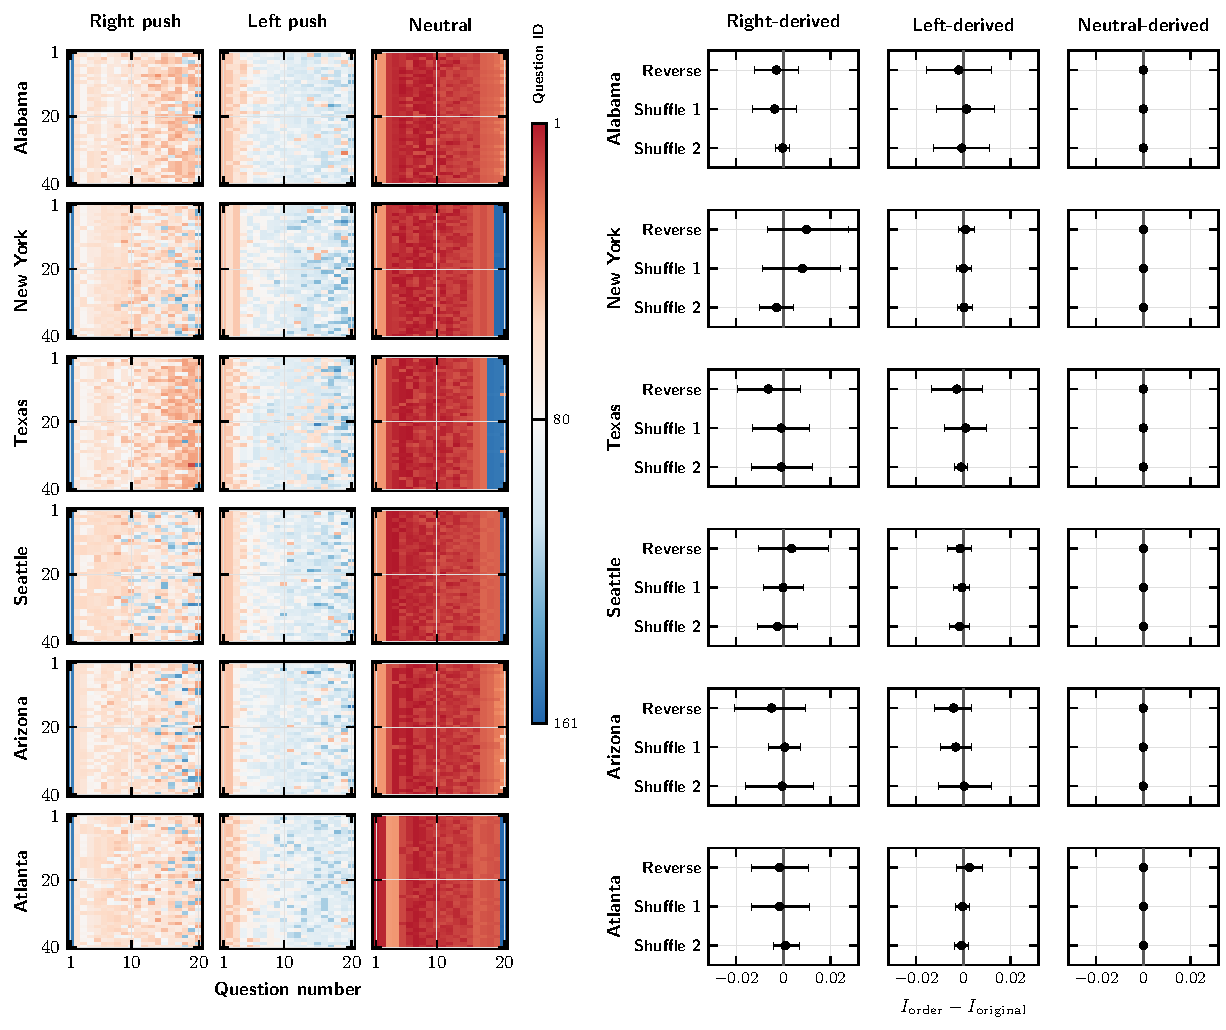
\includegraphics[width=\textwidth]{Figures/External/dtagfig2}%
}{%
\resizebox{\textwidth}{!}{% Inline fallback: 20-question question identities and fixed-order effects.
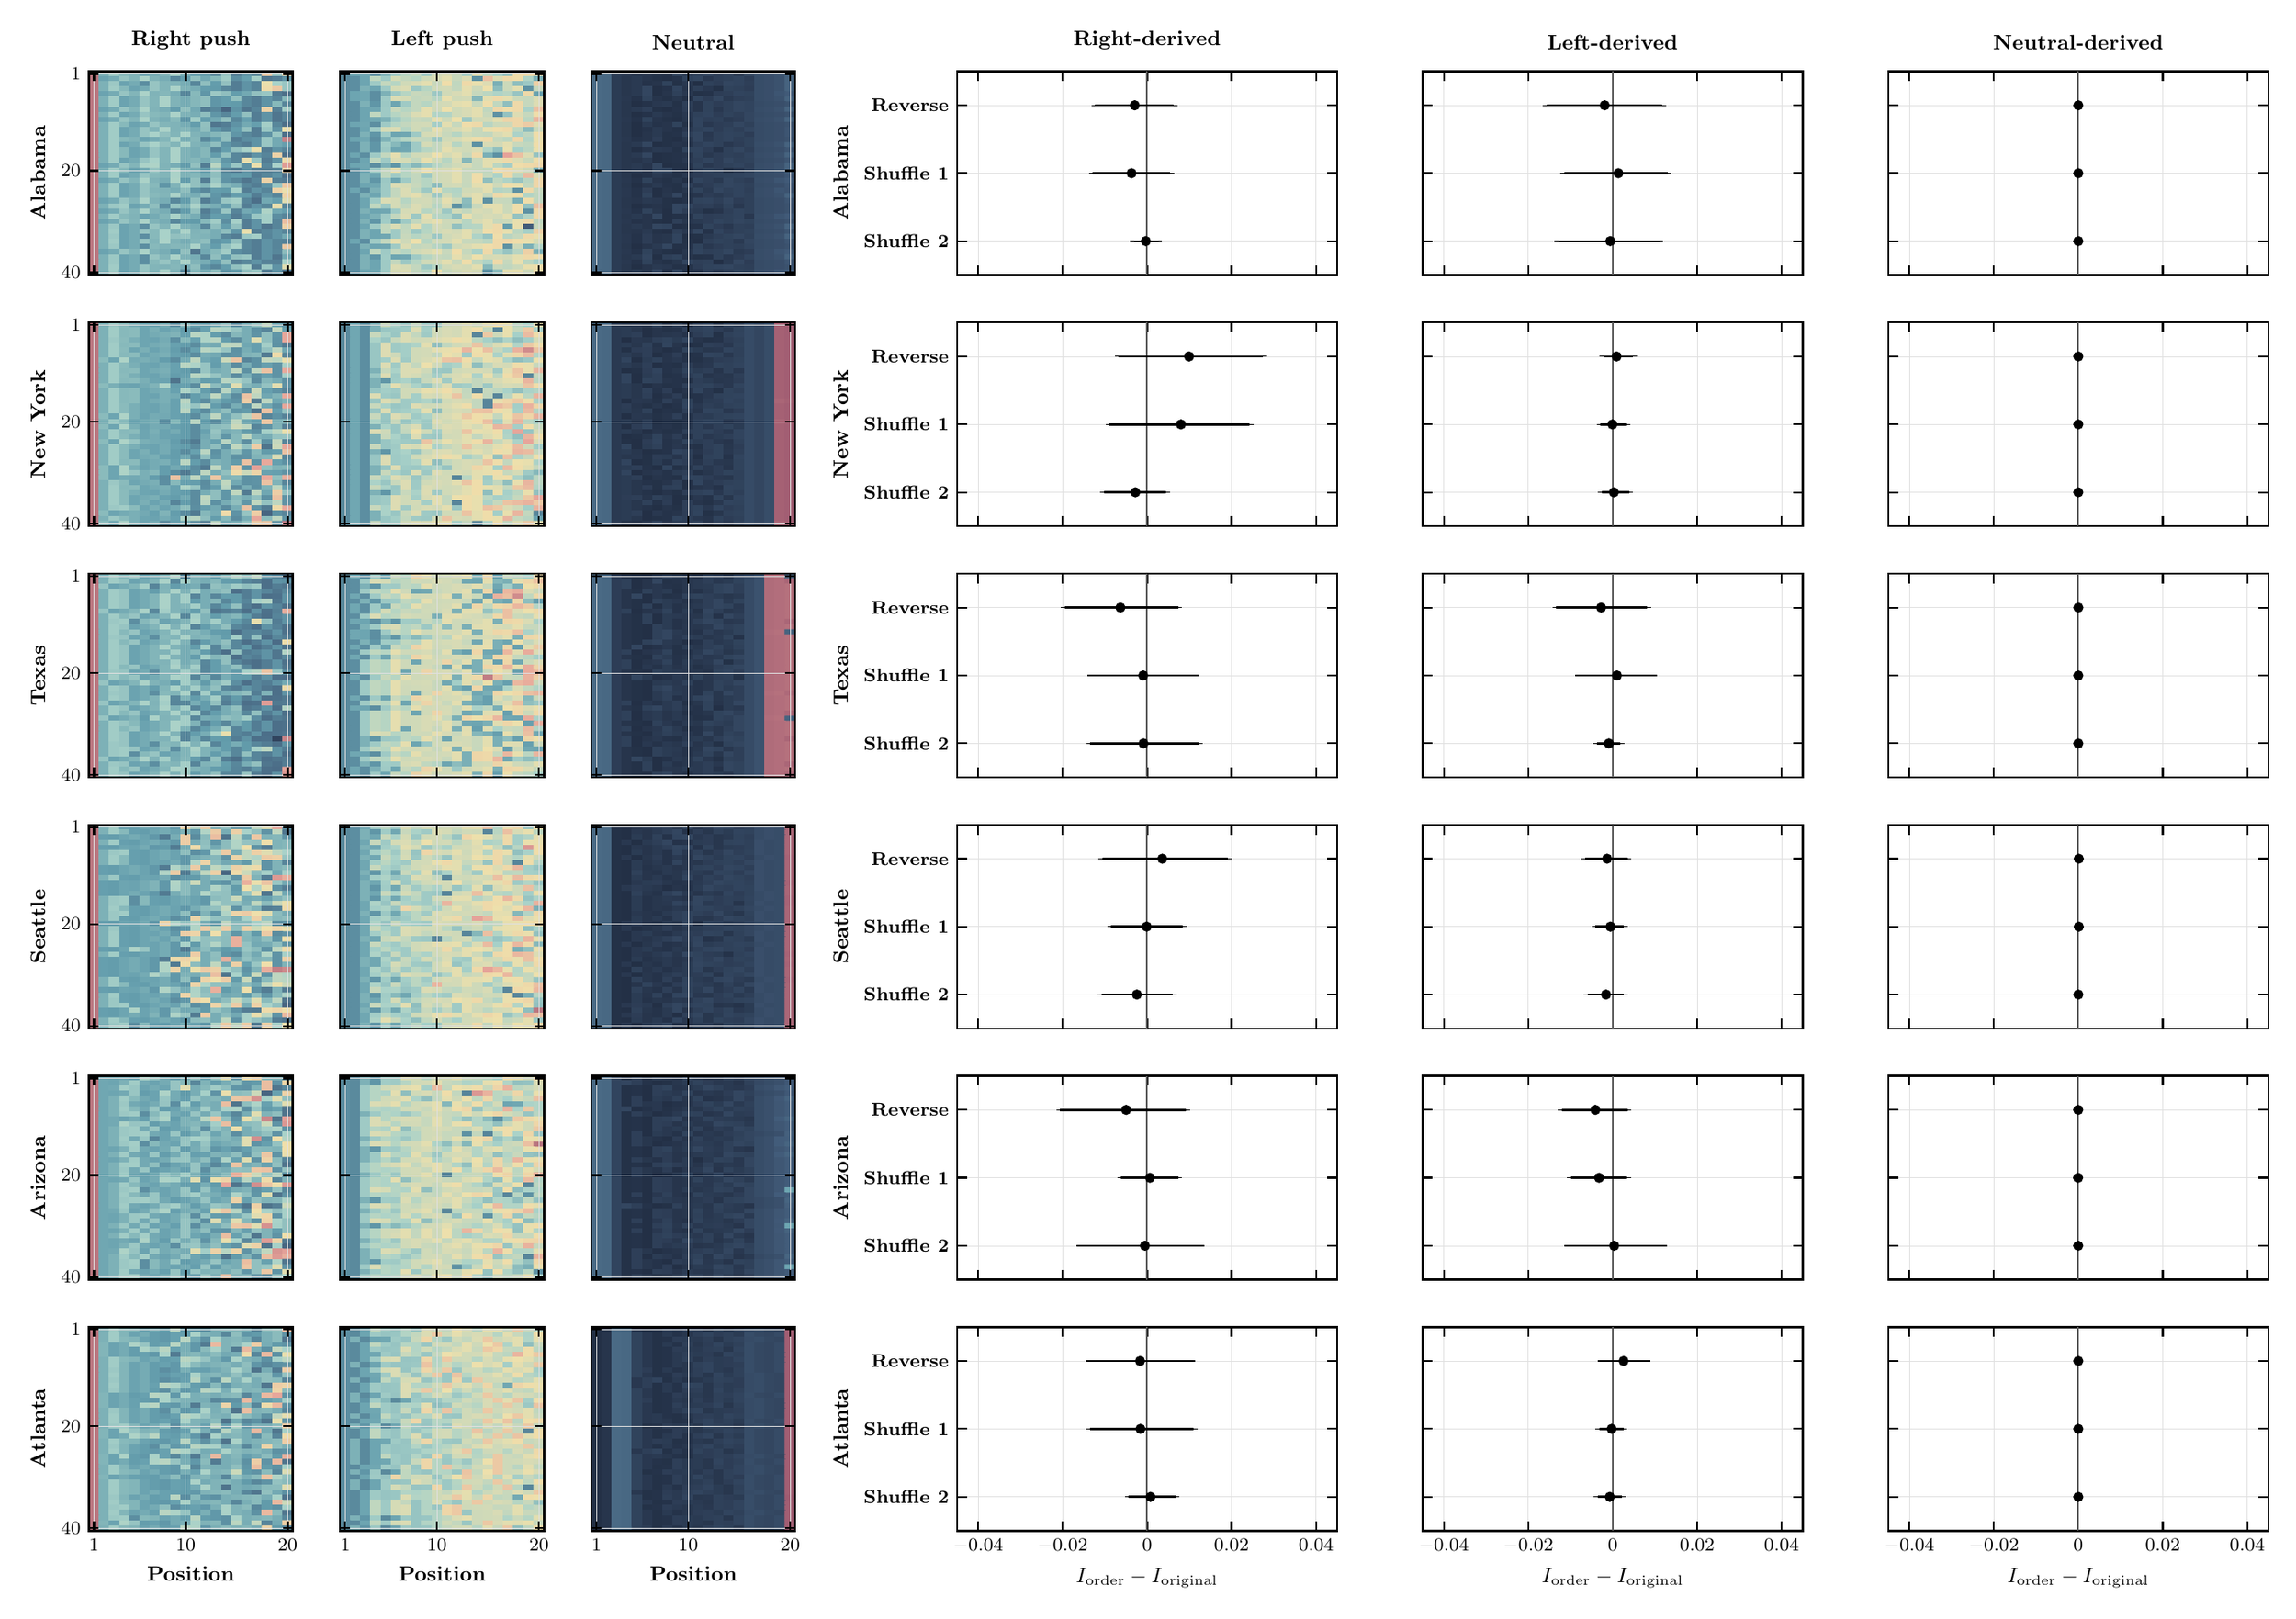
\begin{tikzpicture}

\begin{scope}[shift={(1.9cm,0cm)}]
\begin{groupplot}[
 group style={group size=3 by 6,horizontal sep=.72cm,vertical sep=.72cm},
 scale only axis,publication axis,
 width=3.10cm,height=3.10cm,xmin=.5,xmax=20.5,ymin=.5,ymax=40.5,
 y dir=reverse,axis on top,xtick={1,10,20},ytick={1,20,40},
 xticklabel style={font=\footnotesize\bfseries},yticklabel style={font=\footnotesize\bfseries},
 colormap={questionmap}{
   rgb255=(35,48,70);
   rgb255=(67,93,123);
   rgb255=(100,158,173);
   rgb255=(169,210,201);
   rgb255=(239,224,171);
   rgb255=(231,164,154);
   rgb255=(159,91,113)},
 point meta min=1,point meta max=161
]
\nextgroupplot[title={Right push},ylabel={Alabama},xticklabels={}]
\addplot[matrix plot*,mesh/cols=20,point meta=explicit,mark=none,draw=none] table[row sep=\\,x index=0,y index=1,meta index=2]{
x y value\\
1 1 151\\
2 1 64\\
3 1 78\\
4 1 68\\
5 1 65\\
6 1 57\\
7 1 61\\
8 1 66\\
9 1 82\\
10 1 62\\
11 1 54\\
12 1 53\\
13 1 45\\
14 1 74\\
15 1 41\\
16 1 50\\
17 1 44\\
18 1 118\\
19 1 75\\
20 1 114\\
1 2 151\\
2 2 57\\
3 2 61\\
4 2 74\\
5 2 66\\
6 2 82\\
7 2 65\\
8 2 62\\
9 2 45\\
10 2 54\\
11 2 72\\
12 2 60\\
13 2 68\\
14 2 78\\
15 2 48\\
16 2 55\\
17 2 79\\
18 2 38\\
19 2 41\\
20 2 50\\
1 3 151\\
2 3 64\\
3 3 76\\
4 3 57\\
5 3 61\\
6 3 48\\
7 3 74\\
8 3 66\\
9 3 65\\
10 3 62\\
11 3 45\\
12 3 71\\
13 3 54\\
14 3 72\\
15 3 41\\
16 3 50\\
17 3 44\\
18 3 106\\
19 3 81\\
20 3 75\\
1 4 151\\
2 4 64\\
3 4 78\\
4 4 68\\
5 4 57\\
6 4 61\\
7 4 74\\
8 4 66\\
9 4 82\\
10 4 65\\
11 4 62\\
12 4 54\\
13 4 53\\
14 4 45\\
15 4 41\\
16 4 50\\
17 4 44\\
18 4 110\\
19 4 118\\
20 4 75\\
1 5 151\\
2 5 57\\
3 5 61\\
4 5 74\\
5 5 66\\
6 5 82\\
7 5 65\\
8 5 67\\
9 5 62\\
10 5 45\\
11 5 68\\
12 5 51\\
13 5 76\\
14 5 71\\
15 5 54\\
16 5 60\\
17 5 72\\
18 5 75\\
19 5 41\\
20 5 35\\
1 6 151\\
2 6 64\\
3 6 78\\
4 6 57\\
5 6 61\\
6 6 74\\
7 6 66\\
8 6 82\\
9 6 65\\
10 6 62\\
11 6 67\\
12 6 71\\
13 6 51\\
14 6 54\\
15 6 72\\
16 6 45\\
17 6 41\\
18 6 50\\
19 6 44\\
20 6 68\\
1 7 151\\
2 7 64\\
3 7 78\\
4 7 57\\
5 7 61\\
6 7 74\\
7 7 66\\
8 7 82\\
9 7 65\\
10 7 62\\
11 7 67\\
12 7 71\\
13 7 51\\
14 7 54\\
15 7 53\\
16 7 45\\
17 7 41\\
18 7 50\\
19 7 68\\
20 7 44\\
1 8 151\\
2 8 57\\
3 8 61\\
4 8 74\\
5 8 66\\
6 8 82\\
7 8 65\\
8 8 62\\
9 8 54\\
10 8 72\\
11 8 60\\
12 8 41\\
13 8 45\\
14 8 31\\
15 8 50\\
16 8 38\\
17 8 44\\
18 8 114\\
19 8 42\\
20 8 79\\
1 9 151\\
2 9 64\\
3 9 78\\
4 9 57\\
5 9 61\\
6 9 74\\
7 9 68\\
8 9 66\\
9 9 82\\
10 9 65\\
11 9 62\\
12 9 71\\
13 9 51\\
14 9 45\\
15 9 54\\
16 9 72\\
17 9 41\\
18 9 50\\
19 9 38\\
20 9 44\\
1 10 151\\
2 10 57\\
3 10 61\\
4 10 74\\
5 10 66\\
6 10 82\\
7 10 65\\
8 10 62\\
9 10 68\\
10 10 51\\
11 10 78\\
12 10 54\\
13 10 60\\
14 10 72\\
15 10 45\\
16 10 55\\
17 10 41\\
18 10 50\\
19 10 38\\
20 10 44\\
1 11 151\\
2 11 64\\
3 11 78\\
4 11 68\\
5 11 57\\
6 11 61\\
7 11 74\\
8 11 66\\
9 11 65\\
10 11 62\\
11 11 54\\
12 11 72\\
13 11 38\\
14 11 41\\
15 11 50\\
16 11 60\\
17 11 55\\
18 11 79\\
19 11 45\\
20 11 35\\
1 12 151\\
2 12 64\\
3 12 78\\
4 12 57\\
5 12 61\\
6 12 74\\
7 12 66\\
8 12 82\\
9 12 65\\
10 12 67\\
11 12 62\\
12 12 71\\
13 12 51\\
14 12 45\\
15 12 54\\
16 12 72\\
17 12 41\\
18 12 75\\
19 12 50\\
20 12 106\\
1 13 151\\
2 13 64\\
3 13 78\\
4 13 57\\
5 13 61\\
6 13 74\\
7 13 81\\
8 13 72\\
9 13 66\\
10 13 82\\
11 13 65\\
12 13 62\\
13 13 67\\
14 13 71\\
15 13 51\\
16 13 45\\
17 13 41\\
18 13 50\\
19 13 75\\
20 13 35\\
1 14 151\\
2 14 64\\
3 14 78\\
4 14 68\\
5 14 65\\
6 14 57\\
7 14 61\\
8 14 66\\
9 14 82\\
10 14 62\\
11 14 67\\
12 14 45\\
13 14 54\\
14 14 72\\
15 14 41\\
16 14 48\\
17 14 50\\
18 14 75\\
19 14 60\\
20 14 147\\
1 15 151\\
2 15 64\\
3 15 78\\
4 15 57\\
5 15 61\\
6 15 74\\
7 15 81\\
8 15 72\\
9 15 66\\
10 15 82\\
11 15 65\\
12 15 62\\
13 15 71\\
14 15 51\\
15 15 45\\
16 15 41\\
17 15 50\\
18 15 75\\
19 15 60\\
20 15 55\\
1 16 151\\
2 16 64\\
3 16 78\\
4 16 68\\
5 16 57\\
6 16 61\\
7 16 74\\
8 16 66\\
9 16 82\\
10 16 65\\
11 16 62\\
12 16 67\\
13 16 45\\
14 16 54\\
15 16 72\\
16 16 81\\
17 16 106\\
18 16 41\\
19 16 50\\
20 16 44\\
1 17 151\\
2 17 64\\
3 17 78\\
4 17 68\\
5 17 57\\
6 17 61\\
7 17 74\\
8 17 66\\
9 17 82\\
10 17 65\\
11 17 62\\
12 17 67\\
13 17 54\\
14 17 72\\
15 17 45\\
16 17 41\\
17 17 50\\
18 17 44\\
19 17 114\\
20 17 35\\
1 18 151\\
2 18 64\\
3 18 78\\
4 18 57\\
5 18 61\\
6 18 74\\
7 18 81\\
8 18 66\\
9 18 82\\
10 18 65\\
11 18 67\\
12 18 62\\
13 18 71\\
14 18 51\\
15 18 45\\
16 18 106\\
17 18 75\\
18 18 41\\
19 18 50\\
20 18 110\\
1 19 151\\
2 19 57\\
3 19 61\\
4 19 74\\
5 19 66\\
6 19 82\\
7 19 83\\
8 19 65\\
9 19 62\\
10 19 54\\
11 19 72\\
12 19 41\\
13 19 87\\
14 19 56\\
15 19 75\\
16 19 50\\
17 19 106\\
18 19 45\\
19 19 81\\
20 19 137\\
1 20 151\\
2 20 64\\
3 20 78\\
4 20 68\\
5 20 57\\
6 20 61\\
7 20 74\\
8 20 66\\
9 20 82\\
10 20 65\\
11 20 62\\
12 20 54\\
13 20 72\\
14 20 45\\
15 20 41\\
16 20 50\\
17 20 43\\
18 20 42\\
19 20 44\\
20 20 114\\
1 21 151\\
2 21 64\\
3 21 78\\
4 21 57\\
5 21 61\\
6 21 74\\
7 21 68\\
8 21 66\\
9 21 82\\
10 21 65\\
11 21 67\\
12 21 62\\
13 21 71\\
14 21 51\\
15 21 54\\
16 21 53\\
17 21 41\\
18 21 45\\
19 21 50\\
20 21 35\\
1 22 151\\
2 22 57\\
3 22 61\\
4 22 74\\
5 22 66\\
6 22 82\\
7 22 65\\
8 22 62\\
9 22 83\\
10 22 54\\
11 22 72\\
12 22 41\\
13 22 75\\
14 22 50\\
15 22 45\\
16 22 38\\
17 22 44\\
18 22 114\\
19 22 42\\
20 22 40\\
1 23 151\\
2 23 64\\
3 23 78\\
4 23 57\\
5 23 61\\
6 23 74\\
7 23 68\\
8 23 51\\
9 23 65\\
10 23 81\\
11 23 72\\
12 23 66\\
13 23 82\\
14 23 67\\
15 23 62\\
16 23 45\\
17 23 41\\
18 23 50\\
19 23 75\\
20 23 118\\
1 24 151\\
2 24 64\\
3 24 78\\
4 24 57\\
5 24 61\\
6 24 74\\
7 24 66\\
8 24 65\\
9 24 62\\
10 24 71\\
11 24 51\\
12 24 45\\
13 24 54\\
14 24 53\\
15 24 80\\
16 24 41\\
17 24 50\\
18 24 44\\
19 24 114\\
20 24 106\\
1 25 151\\
2 25 64\\
3 25 78\\
4 25 57\\
5 25 61\\
6 25 74\\
7 25 68\\
8 25 66\\
9 25 82\\
10 25 65\\
11 25 62\\
12 25 71\\
13 25 51\\
14 25 45\\
15 25 54\\
16 25 53\\
17 25 41\\
18 25 50\\
19 25 44\\
20 25 114\\
1 26 151\\
2 26 57\\
3 26 61\\
4 26 74\\
5 26 66\\
6 26 82\\
7 26 65\\
8 26 62\\
9 26 45\\
10 26 54\\
11 26 72\\
12 26 41\\
13 26 50\\
14 26 75\\
15 26 79\\
16 26 44\\
17 26 35\\
18 26 60\\
19 26 55\\
20 26 102\\
1 27 151\\
2 27 64\\
3 27 76\\
4 27 78\\
5 27 57\\
6 27 61\\
7 27 71\\
8 27 48\\
9 27 74\\
10 27 66\\
11 27 82\\
12 27 65\\
13 27 62\\
14 27 54\\
15 27 72\\
16 27 41\\
17 27 50\\
18 27 45\\
19 27 106\\
20 27 44\\
1 28 151\\
2 28 57\\
3 28 61\\
4 28 74\\
5 28 66\\
6 28 82\\
7 28 65\\
8 28 62\\
9 28 45\\
10 28 54\\
11 28 72\\
12 28 41\\
13 28 50\\
14 28 75\\
15 28 44\\
16 28 60\\
17 28 56\\
18 28 83\\
19 28 59\\
20 28 55\\
1 29 151\\
2 29 64\\
3 29 78\\
4 29 68\\
5 29 65\\
6 29 57\\
7 29 61\\
8 29 66\\
9 29 82\\
10 29 67\\
11 29 62\\
12 29 45\\
13 29 54\\
14 29 53\\
15 29 41\\
16 29 50\\
17 29 75\\
18 29 79\\
19 29 48\\
20 29 44\\
1 30 151\\
2 30 57\\
3 30 61\\
4 30 74\\
5 30 66\\
6 30 82\\
7 30 65\\
8 30 62\\
9 30 45\\
10 30 54\\
11 30 53\\
12 30 68\\
13 30 78\\
14 30 48\\
15 30 80\\
16 30 41\\
17 30 50\\
18 30 79\\
19 30 44\\
20 30 123\\
1 31 151\\
2 31 64\\
3 31 76\\
4 31 57\\
5 31 61\\
6 31 48\\
7 31 74\\
8 31 66\\
9 31 82\\
10 31 65\\
11 31 62\\
12 31 45\\
13 31 71\\
14 31 54\\
15 31 72\\
16 31 41\\
17 31 50\\
18 31 38\\
19 31 44\\
20 31 114\\
1 32 151\\
2 32 64\\
3 32 78\\
4 32 57\\
5 32 61\\
6 32 74\\
7 32 68\\
8 32 81\\
9 32 66\\
10 32 82\\
11 32 65\\
12 32 67\\
13 32 62\\
14 32 71\\
15 32 51\\
16 32 106\\
17 32 41\\
18 32 45\\
19 32 50\\
20 32 44\\
1 33 151\\
2 33 64\\
3 33 76\\
4 33 57\\
5 33 61\\
6 33 48\\
7 33 68\\
8 33 81\\
9 33 72\\
10 33 74\\
11 33 66\\
12 33 65\\
13 33 62\\
14 33 45\\
15 33 41\\
16 33 75\\
17 33 79\\
18 33 44\\
19 33 50\\
20 33 60\\
1 34 151\\
2 34 64\\
3 34 78\\
4 34 57\\
5 34 61\\
6 34 74\\
7 34 66\\
8 34 82\\
9 34 65\\
10 34 62\\
11 34 67\\
12 34 71\\
13 34 51\\
14 34 54\\
15 34 72\\
16 34 45\\
17 34 41\\
18 34 50\\
19 34 44\\
20 34 43\\
1 35 151\\
2 35 64\\
3 35 76\\
4 35 57\\
5 35 61\\
6 35 48\\
7 35 68\\
8 35 65\\
9 35 67\\
10 35 66\\
11 35 82\\
12 35 62\\
13 35 54\\
14 35 72\\
15 35 81\\
16 35 45\\
17 35 41\\
18 35 50\\
19 35 44\\
20 35 118\\
1 36 151\\
2 36 57\\
3 36 61\\
4 36 74\\
5 36 66\\
6 36 82\\
7 36 65\\
8 36 62\\
9 36 54\\
10 36 72\\
11 36 38\\
12 36 60\\
13 36 68\\
14 36 78\\
15 36 48\\
16 36 44\\
17 36 41\\
18 36 50\\
19 36 45\\
20 36 70\\
1 37 151\\
2 37 64\\
3 37 76\\
4 37 57\\
5 37 61\\
6 37 48\\
7 37 74\\
8 37 66\\
9 37 82\\
10 37 65\\
11 37 62\\
12 37 45\\
13 37 71\\
14 37 54\\
15 37 72\\
16 37 75\\
17 37 41\\
18 37 50\\
19 37 38\\
20 37 60\\
1 38 151\\
2 38 64\\
3 38 76\\
4 38 57\\
5 38 61\\
6 38 48\\
7 38 68\\
8 38 74\\
9 38 66\\
10 38 82\\
11 38 65\\
12 38 62\\
13 38 54\\
14 38 72\\
15 38 41\\
16 38 45\\
17 38 50\\
18 38 43\\
19 38 42\\
20 38 81\\
1 39 151\\
2 39 64\\
3 39 78\\
4 39 57\\
5 39 61\\
6 39 74\\
7 39 66\\
8 39 65\\
9 39 67\\
10 39 62\\
11 39 71\\
12 39 51\\
13 39 45\\
14 39 54\\
15 39 72\\
16 39 81\\
17 39 41\\
18 39 75\\
19 39 50\\
20 39 102\\
1 40 151\\
2 40 64\\
3 40 78\\
4 40 57\\
5 40 61\\
6 40 74\\
7 40 66\\
8 40 82\\
9 40 65\\
10 40 45\\
11 40 67\\
12 40 62\\
13 40 71\\
14 40 51\\
15 40 54\\
16 40 72\\
17 40 75\\
18 40 41\\
19 40 50\\
20 40 38\\
};
\nextgroupplot[title={Left push},yticklabels={},xticklabels={}]
\addplot[matrix plot*,mesh/cols=20,point meta=explicit,mark=none,draw=none] table[row sep=\\,x index=0,y index=1,meta index=2]{
x y value\\
1 1 46\\
2 1 58\\
3 1 59\\
4 1 48\\
5 1 64\\
6 1 77\\
7 1 86\\
8 1 91\\
9 1 76\\
10 1 96\\
11 1 99\\
12 1 92\\
13 1 79\\
14 1 103\\
15 1 88\\
16 1 80\\
17 1 72\\
18 1 109\\
19 1 111\\
20 1 112\\
1 2 46\\
2 2 48\\
3 2 58\\
4 2 90\\
5 2 77\\
6 2 98\\
7 2 91\\
8 2 86\\
9 2 96\\
10 2 99\\
11 2 103\\
12 2 93\\
13 2 100\\
14 2 49\\
15 2 122\\
16 2 101\\
17 2 111\\
18 2 109\\
19 2 84\\
20 2 63\\
1 3 46\\
2 3 48\\
3 3 58\\
4 3 77\\
5 3 91\\
6 3 86\\
7 3 96\\
8 3 99\\
9 3 103\\
10 3 93\\
11 3 109\\
12 3 90\\
13 3 111\\
14 3 105\\
15 3 101\\
16 3 63\\
17 3 94\\
18 3 71\\
19 3 76\\
20 3 115\\
1 4 46\\
2 4 48\\
3 4 64\\
4 4 58\\
5 4 77\\
6 4 98\\
7 4 100\\
8 4 76\\
9 4 86\\
10 4 96\\
11 4 97\\
12 4 91\\
13 4 104\\
14 4 95\\
15 4 107\\
16 4 70\\
17 4 94\\
18 4 103\\
19 4 49\\
20 4 93\\
1 5 46\\
2 5 58\\
3 5 59\\
4 5 48\\
5 5 64\\
6 5 77\\
7 5 86\\
8 5 93\\
9 5 91\\
10 5 76\\
11 5 96\\
12 5 99\\
13 5 103\\
14 5 92\\
15 5 88\\
16 5 83\\
17 5 87\\
18 5 74\\
19 5 111\\
20 5 56\\
1 6 46\\
2 6 58\\
3 6 59\\
4 6 48\\
5 6 77\\
6 6 100\\
7 6 98\\
8 6 91\\
9 6 93\\
10 6 86\\
11 6 105\\
12 6 96\\
13 6 97\\
14 6 67\\
15 6 103\\
16 6 111\\
17 6 104\\
18 6 94\\
19 6 92\\
20 6 101\\
1 7 46\\
2 7 48\\
3 7 64\\
4 7 51\\
5 7 76\\
6 7 58\\
7 7 77\\
8 7 91\\
9 7 86\\
10 7 96\\
11 7 97\\
12 7 103\\
13 7 105\\
14 7 93\\
15 7 109\\
16 7 90\\
17 7 71\\
18 7 111\\
19 7 92\\
20 7 101\\
1 8 46\\
2 8 48\\
3 8 58\\
4 8 59\\
5 8 77\\
6 8 93\\
7 8 86\\
8 8 91\\
9 8 104\\
10 8 95\\
11 8 107\\
12 8 96\\
13 8 99\\
14 8 103\\
15 8 90\\
16 8 112\\
17 8 109\\
18 8 111\\
19 8 82\\
20 8 122\\
1 9 46\\
2 9 48\\
3 9 58\\
4 9 90\\
5 9 77\\
6 9 86\\
7 9 91\\
8 9 100\\
9 9 104\\
10 9 84\\
11 9 85\\
12 9 96\\
13 9 99\\
14 9 103\\
15 9 93\\
16 9 49\\
17 9 73\\
18 9 101\\
19 9 92\\
20 9 109\\
1 10 46\\
2 10 48\\
3 10 58\\
4 10 59\\
5 10 64\\
6 10 77\\
7 10 86\\
8 10 93\\
9 10 91\\
10 10 104\\
11 10 95\\
12 10 107\\
13 10 76\\
14 10 96\\
15 10 97\\
16 10 103\\
17 10 113\\
18 10 112\\
19 10 88\\
20 10 127\\
1 11 46\\
2 11 58\\
3 11 59\\
4 11 48\\
5 11 77\\
6 11 86\\
7 11 91\\
8 11 96\\
9 11 97\\
10 11 79\\
11 11 103\\
12 11 92\\
13 11 109\\
14 11 111\\
15 11 87\\
16 11 94\\
17 11 95\\
18 11 112\\
19 11 117\\
20 11 102\\
1 12 46\\
2 12 48\\
3 12 58\\
4 12 77\\
5 12 98\\
6 12 100\\
7 12 86\\
8 12 96\\
9 12 91\\
10 12 104\\
11 12 95\\
12 12 99\\
13 12 103\\
14 12 93\\
15 12 105\\
16 12 109\\
17 12 111\\
18 12 90\\
19 12 70\\
20 12 94\\
1 13 46\\
2 13 48\\
3 13 64\\
4 13 51\\
5 13 78\\
6 13 58\\
7 13 59\\
8 13 77\\
9 13 98\\
10 13 100\\
11 13 93\\
12 13 86\\
13 13 96\\
14 13 92\\
15 13 91\\
16 13 99\\
17 13 103\\
18 13 82\\
19 13 89\\
20 13 109\\
1 14 46\\
2 14 58\\
3 14 59\\
4 14 48\\
5 14 64\\
6 14 77\\
7 14 86\\
8 14 93\\
9 14 91\\
10 14 76\\
11 14 96\\
12 14 99\\
13 14 103\\
14 14 109\\
15 14 111\\
16 14 92\\
17 14 88\\
18 14 112\\
19 14 85\\
20 14 106\\
1 15 46\\
2 15 48\\
3 15 64\\
4 15 51\\
5 15 78\\
6 15 68\\
7 15 58\\
8 15 77\\
9 15 98\\
10 15 91\\
11 15 100\\
12 15 86\\
13 15 96\\
14 15 49\\
15 15 99\\
16 15 97\\
17 15 103\\
18 15 93\\
19 15 90\\
20 15 109\\
1 16 46\\
2 16 48\\
3 16 64\\
4 16 51\\
5 16 76\\
6 16 58\\
7 16 59\\
8 16 77\\
9 16 86\\
10 16 91\\
11 16 104\\
12 16 98\\
13 16 96\\
14 16 100\\
15 16 84\\
16 16 72\\
17 16 105\\
18 16 80\\
19 16 88\\
20 16 106\\
1 17 46\\
2 17 58\\
3 17 48\\
4 17 77\\
5 17 91\\
6 17 104\\
7 17 86\\
8 17 96\\
9 17 97\\
10 17 107\\
11 17 98\\
12 17 103\\
13 17 93\\
14 17 111\\
15 17 63\\
16 17 49\\
17 17 135\\
18 17 122\\
19 17 101\\
20 17 73\\
1 18 46\\
2 18 48\\
3 18 58\\
4 18 90\\
5 18 77\\
6 18 100\\
7 18 98\\
8 18 91\\
9 18 105\\
10 18 96\\
11 18 86\\
12 18 99\\
13 18 67\\
14 18 93\\
15 18 103\\
16 18 104\\
17 18 111\\
18 18 101\\
19 18 94\\
20 18 109\\
1 19 46\\
2 19 58\\
3 19 59\\
4 19 48\\
5 19 64\\
6 19 51\\
7 19 78\\
8 19 68\\
9 19 77\\
10 19 86\\
11 19 91\\
12 19 96\\
13 19 99\\
14 19 92\\
15 19 103\\
16 19 88\\
17 19 79\\
18 19 109\\
19 19 111\\
20 19 112\\
1 20 46\\
2 20 48\\
3 20 58\\
4 20 77\\
5 20 91\\
6 20 104\\
7 20 86\\
8 20 96\\
9 20 107\\
10 20 98\\
11 20 99\\
12 20 103\\
13 20 93\\
14 20 92\\
15 20 90\\
16 20 109\\
17 20 111\\
18 20 101\\
19 20 95\\
20 20 63\\
1 21 46\\
2 21 48\\
3 21 64\\
4 21 58\\
5 21 90\\
6 21 77\\
7 21 86\\
8 21 91\\
9 21 76\\
10 21 96\\
11 21 97\\
12 21 103\\
13 21 93\\
14 21 109\\
15 21 92\\
16 21 82\\
17 21 111\\
18 21 88\\
19 21 124\\
20 21 101\\
1 22 46\\
2 22 48\\
3 22 64\\
4 22 51\\
5 22 76\\
6 22 58\\
7 22 77\\
8 22 91\\
9 22 86\\
10 22 96\\
11 22 97\\
12 22 103\\
13 22 93\\
14 22 109\\
15 22 71\\
16 22 90\\
17 22 83\\
18 22 74\\
19 22 87\\
20 22 112\\
1 23 46\\
2 23 48\\
3 23 58\\
4 23 59\\
5 23 77\\
6 23 100\\
7 23 98\\
8 23 93\\
9 23 86\\
10 23 70\\
11 23 96\\
12 23 97\\
13 23 92\\
14 23 103\\
15 23 104\\
16 23 95\\
17 23 109\\
18 23 105\\
19 23 91\\
20 23 112\\
1 24 46\\
2 24 58\\
3 24 48\\
4 24 64\\
5 24 77\\
6 24 91\\
7 24 100\\
8 24 90\\
9 24 76\\
10 24 104\\
11 24 86\\
12 24 84\\
13 24 96\\
14 24 97\\
15 24 103\\
16 24 85\\
17 24 87\\
18 24 49\\
19 24 111\\
20 24 92\\
1 25 46\\
2 25 48\\
3 25 64\\
4 25 58\\
5 25 77\\
6 25 91\\
7 25 100\\
8 25 104\\
9 25 95\\
10 25 76\\
11 25 96\\
12 25 86\\
13 25 99\\
14 25 103\\
15 25 93\\
16 25 111\\
17 25 105\\
18 25 109\\
19 25 84\\
20 25 90\\
1 26 46\\
2 26 48\\
3 26 58\\
4 26 77\\
5 26 100\\
6 26 98\\
7 26 86\\
8 26 96\\
9 26 97\\
10 26 91\\
11 26 104\\
12 26 95\\
13 26 70\\
14 26 103\\
15 26 49\\
16 26 93\\
17 26 92\\
18 26 63\\
19 26 109\\
20 26 90\\
1 27 46\\
2 27 48\\
3 27 58\\
4 27 90\\
5 27 77\\
6 27 98\\
7 27 91\\
8 27 100\\
9 27 96\\
10 27 86\\
11 27 99\\
12 27 49\\
13 27 67\\
14 27 93\\
15 27 104\\
16 27 103\\
17 27 94\\
18 27 109\\
19 27 73\\
20 27 122\\
1 28 46\\
2 28 48\\
3 28 64\\
4 28 58\\
5 28 59\\
6 28 77\\
7 28 98\\
8 28 100\\
9 28 86\\
10 28 92\\
11 28 76\\
12 28 96\\
13 28 91\\
14 28 99\\
15 28 97\\
16 28 103\\
17 28 94\\
18 28 109\\
19 28 49\\
20 28 111\\
1 29 46\\
2 29 48\\
3 29 58\\
4 29 64\\
5 29 77\\
6 29 91\\
7 29 100\\
8 29 76\\
9 29 104\\
10 29 86\\
11 29 84\\
12 29 72\\
13 29 105\\
14 29 96\\
15 29 99\\
16 29 97\\
17 29 103\\
18 29 73\\
19 29 85\\
20 29 111\\
1 30 46\\
2 30 48\\
3 30 64\\
4 30 51\\
5 30 78\\
6 30 58\\
7 30 77\\
8 30 91\\
9 30 100\\
10 30 104\\
11 30 95\\
12 30 96\\
13 30 86\\
14 30 99\\
15 30 103\\
16 30 93\\
17 30 94\\
18 30 105\\
19 30 111\\
20 30 90\\
1 31 46\\
2 31 48\\
3 31 58\\
4 31 77\\
5 31 91\\
6 31 100\\
7 31 90\\
8 31 104\\
9 31 84\\
10 31 97\\
11 31 94\\
12 31 72\\
13 31 85\\
14 31 86\\
15 31 103\\
16 31 111\\
17 31 54\\
18 31 105\\
19 31 26\\
20 31 93\\
1 32 46\\
2 32 48\\
3 32 64\\
4 32 58\\
5 32 90\\
6 32 77\\
7 32 91\\
8 32 76\\
9 32 86\\
10 32 96\\
11 32 99\\
12 32 97\\
13 32 103\\
14 32 93\\
15 32 109\\
16 32 111\\
17 32 105\\
18 32 88\\
19 32 80\\
20 32 115\\
1 33 46\\
2 33 48\\
3 33 64\\
4 33 58\\
5 33 59\\
6 33 77\\
7 33 93\\
8 33 86\\
9 33 91\\
10 33 76\\
11 33 96\\
12 33 99\\
13 33 103\\
14 33 83\\
15 33 74\\
16 33 109\\
17 33 87\\
18 33 92\\
19 33 111\\
20 33 105\\
1 34 46\\
2 34 58\\
3 34 48\\
4 34 77\\
5 34 91\\
6 34 104\\
7 34 95\\
8 34 107\\
9 34 86\\
10 34 96\\
11 34 97\\
12 34 103\\
13 34 93\\
14 34 92\\
15 34 88\\
16 34 111\\
17 34 112\\
18 34 109\\
19 34 105\\
20 34 98\\
1 35 46\\
2 35 48\\
3 35 64\\
4 35 58\\
5 35 59\\
6 35 77\\
7 35 100\\
8 35 91\\
9 35 93\\
10 35 86\\
11 35 76\\
12 35 96\\
13 35 99\\
14 35 103\\
15 35 109\\
16 35 111\\
17 35 49\\
18 35 95\\
19 35 63\\
20 35 84\\
1 36 46\\
2 36 48\\
3 36 58\\
4 36 90\\
5 36 77\\
6 36 91\\
7 36 86\\
8 36 96\\
9 36 99\\
10 36 103\\
11 36 93\\
12 36 109\\
13 36 92\\
14 36 82\\
15 36 111\\
16 36 83\\
17 36 74\\
18 36 87\\
19 36 115\\
20 36 63\\
1 37 46\\
2 37 48\\
3 37 64\\
4 37 51\\
5 37 78\\
6 37 58\\
7 37 59\\
8 37 77\\
9 37 86\\
10 37 93\\
11 37 91\\
12 37 104\\
13 37 96\\
14 37 107\\
15 37 98\\
16 37 99\\
17 37 97\\
18 37 103\\
19 37 111\\
20 37 109\\
1 38 46\\
2 38 48\\
3 38 64\\
4 38 58\\
5 38 77\\
6 38 91\\
7 38 76\\
8 38 86\\
9 38 96\\
10 38 97\\
11 38 103\\
12 38 93\\
13 38 109\\
14 38 90\\
15 38 83\\
16 38 111\\
17 38 92\\
18 38 105\\
19 38 88\\
20 38 80\\
1 39 46\\
2 39 48\\
3 39 64\\
4 39 58\\
5 39 77\\
6 39 100\\
7 39 98\\
8 39 91\\
9 39 76\\
10 39 86\\
11 39 96\\
12 39 99\\
13 39 97\\
14 39 103\\
15 39 67\\
16 39 93\\
17 39 90\\
18 39 94\\
19 39 105\\
20 39 109\\
1 40 46\\
2 40 48\\
3 40 58\\
4 40 59\\
5 40 77\\
6 40 98\\
7 40 100\\
8 40 91\\
9 40 86\\
10 40 107\\
11 40 92\\
12 40 96\\
13 40 99\\
14 40 97\\
15 40 49\\
16 40 70\\
17 40 103\\
18 40 104\\
19 40 95\\
20 40 109\\
};
\nextgroupplot[title={Neutral},yticklabels={},xticklabels={}]
\addplot[matrix plot*,mesh/cols=20,point meta=explicit,mark=none,draw=none] table[row sep=\\,x index=0,y index=1,meta index=2]{
x y value\\
1 1 33\\
2 1 32\\
3 1 8\\
4 1 6\\
5 1 3\\
6 1 4\\
7 1 2\\
8 1 1\\
9 1 12\\
10 1 7\\
11 1 10\\
12 1 13\\
13 1 9\\
14 1 11\\
15 1 5\\
16 1 14\\
17 1 18\\
18 1 19\\
19 1 21\\
20 1 30\\
1 2 33\\
2 2 32\\
3 2 8\\
4 2 5\\
5 2 7\\
6 2 4\\
7 2 2\\
8 2 1\\
9 2 3\\
10 2 12\\
11 2 14\\
12 2 6\\
13 2 10\\
14 2 11\\
15 2 13\\
16 2 9\\
17 2 18\\
18 2 19\\
19 2 21\\
20 2 30\\
1 3 33\\
2 3 32\\
3 3 8\\
4 3 5\\
5 3 7\\
6 3 3\\
7 3 4\\
8 3 12\\
9 3 2\\
10 3 6\\
11 3 1\\
12 3 11\\
13 3 9\\
14 3 14\\
15 3 13\\
16 3 10\\
17 3 18\\
18 3 19\\
19 3 21\\
20 3 30\\
1 4 33\\
2 4 32\\
3 4 8\\
4 4 5\\
5 4 7\\
6 4 14\\
7 4 1\\
8 4 3\\
9 4 13\\
10 4 4\\
11 4 10\\
12 4 6\\
13 4 2\\
14 4 12\\
15 4 11\\
16 4 9\\
17 4 18\\
18 4 19\\
19 4 21\\
20 4 30\\
1 5 33\\
2 5 32\\
3 5 8\\
4 5 5\\
5 5 7\\
6 5 14\\
7 5 1\\
8 5 4\\
9 5 11\\
10 5 6\\
11 5 2\\
12 5 3\\
13 5 9\\
14 5 10\\
15 5 13\\
16 5 12\\
17 5 18\\
18 5 19\\
19 5 23\\
20 5 26\\
1 6 33\\
2 6 32\\
3 6 8\\
4 6 6\\
5 6 3\\
6 6 12\\
7 6 4\\
8 6 2\\
9 6 5\\
10 6 1\\
11 6 13\\
12 6 9\\
13 6 14\\
14 6 7\\
15 6 10\\
16 6 11\\
17 6 18\\
18 6 19\\
19 6 21\\
20 6 30\\
1 7 33\\
2 7 32\\
3 7 8\\
4 7 5\\
5 7 1\\
6 7 3\\
7 7 6\\
8 7 7\\
9 7 2\\
10 7 10\\
11 7 4\\
12 7 12\\
13 7 9\\
14 7 11\\
15 7 14\\
16 7 13\\
17 7 17\\
18 7 18\\
19 7 19\\
20 7 21\\
1 8 33\\
2 8 32\\
3 8 8\\
4 8 5\\
5 8 7\\
6 8 10\\
7 8 2\\
8 8 1\\
9 8 3\\
10 8 9\\
11 8 4\\
12 8 12\\
13 8 6\\
14 8 11\\
15 8 14\\
16 8 13\\
17 8 18\\
18 8 19\\
19 8 21\\
20 8 30\\
1 9 33\\
2 9 32\\
3 9 8\\
4 9 5\\
5 9 1\\
6 9 3\\
7 9 7\\
8 9 4\\
9 9 2\\
10 9 6\\
11 9 11\\
12 9 13\\
13 9 9\\
14 9 12\\
15 9 10\\
16 9 14\\
17 9 17\\
18 9 18\\
19 9 19\\
20 9 21\\
1 10 33\\
2 10 32\\
3 10 8\\
4 10 6\\
5 10 3\\
6 10 12\\
7 10 4\\
8 10 2\\
9 10 1\\
10 10 5\\
11 10 13\\
12 10 10\\
13 10 11\\
14 10 7\\
15 10 9\\
16 10 14\\
17 10 18\\
18 10 19\\
19 10 21\\
20 10 30\\
1 11 33\\
2 11 32\\
3 11 8\\
4 11 5\\
5 11 1\\
6 11 7\\
7 11 3\\
8 11 4\\
9 11 12\\
10 11 2\\
11 11 13\\
12 11 6\\
13 11 9\\
14 11 10\\
15 11 14\\
16 11 11\\
17 11 17\\
18 11 18\\
19 11 19\\
20 11 21\\
1 12 33\\
2 12 32\\
3 12 8\\
4 12 5\\
5 12 1\\
6 12 3\\
7 12 7\\
8 12 4\\
9 12 2\\
10 12 6\\
11 12 11\\
12 12 13\\
13 12 9\\
14 12 12\\
15 12 10\\
16 12 14\\
17 12 17\\
18 12 18\\
19 12 19\\
20 12 23\\
1 13 33\\
2 13 32\\
3 13 8\\
4 13 5\\
5 13 1\\
6 13 4\\
7 13 7\\
8 13 2\\
9 13 3\\
10 13 10\\
11 13 14\\
12 13 6\\
13 13 11\\
14 13 13\\
15 13 12\\
16 13 9\\
17 13 17\\
18 13 18\\
19 13 19\\
20 13 23\\
1 14 33\\
2 14 32\\
3 14 8\\
4 14 6\\
5 14 3\\
6 14 4\\
7 14 9\\
8 14 2\\
9 14 1\\
10 14 5\\
11 14 14\\
12 14 7\\
13 14 11\\
14 14 13\\
15 14 10\\
16 14 12\\
17 14 17\\
18 14 18\\
19 14 19\\
20 14 21\\
1 15 33\\
2 15 32\\
3 15 8\\
4 15 5\\
5 15 7\\
6 15 14\\
7 15 1\\
8 15 2\\
9 15 4\\
10 15 3\\
11 15 10\\
12 15 13\\
13 15 11\\
14 15 6\\
15 15 9\\
16 15 12\\
17 15 18\\
18 15 19\\
19 15 21\\
20 15 30\\
1 16 33\\
2 16 32\\
3 16 8\\
4 16 5\\
5 16 1\\
6 16 4\\
7 16 7\\
8 16 6\\
9 16 2\\
10 16 12\\
11 16 13\\
12 16 9\\
13 16 3\\
14 16 11\\
15 16 14\\
16 16 10\\
17 16 17\\
18 16 18\\
19 16 19\\
20 16 23\\
1 17 33\\
2 17 32\\
3 17 8\\
4 17 5\\
5 17 7\\
6 17 14\\
7 17 1\\
8 17 2\\
9 17 3\\
10 17 4\\
11 17 12\\
12 17 6\\
13 17 9\\
14 17 11\\
15 17 10\\
16 17 13\\
17 17 18\\
18 17 19\\
19 17 21\\
20 17 30\\
1 18 33\\
2 18 32\\
3 18 8\\
4 18 5\\
5 18 4\\
6 18 7\\
7 18 1\\
8 18 2\\
9 18 3\\
10 18 6\\
11 18 10\\
12 18 13\\
13 18 9\\
14 18 14\\
15 18 11\\
16 18 12\\
17 18 17\\
18 18 18\\
19 18 19\\
20 18 23\\
1 19 33\\
2 19 32\\
3 19 8\\
4 19 5\\
5 19 7\\
6 19 4\\
7 19 14\\
8 19 1\\
9 19 2\\
10 19 3\\
11 19 12\\
12 19 6\\
13 19 9\\
14 19 11\\
15 19 13\\
16 19 10\\
17 19 18\\
18 19 19\\
19 19 21\\
20 19 30\\
1 20 33\\
2 20 32\\
3 20 8\\
4 20 5\\
5 20 7\\
6 20 4\\
7 20 14\\
8 20 13\\
9 20 3\\
10 20 1\\
11 20 9\\
12 20 12\\
13 20 10\\
14 20 2\\
15 20 6\\
16 20 11\\
17 20 18\\
18 20 19\\
19 20 21\\
20 20 30\\
1 21 33\\
2 21 32\\
3 21 8\\
4 21 5\\
5 21 1\\
6 21 3\\
7 21 7\\
8 21 4\\
9 21 2\\
10 21 6\\
11 21 9\\
12 21 10\\
13 21 11\\
14 21 12\\
15 21 13\\
16 21 14\\
17 21 17\\
18 21 18\\
19 21 19\\
20 21 23\\
1 22 33\\
2 22 32\\
3 22 8\\
4 22 6\\
5 22 3\\
6 22 12\\
7 22 4\\
8 22 2\\
9 22 5\\
10 22 1\\
11 22 13\\
12 22 10\\
13 22 7\\
14 22 14\\
15 22 11\\
16 22 9\\
17 22 18\\
18 22 19\\
19 22 23\\
20 22 26\\
1 23 33\\
2 23 32\\
3 23 8\\
4 23 5\\
5 23 1\\
6 23 4\\
7 23 7\\
8 23 3\\
9 23 2\\
10 23 10\\
11 23 6\\
12 23 9\\
13 23 12\\
14 23 14\\
15 23 13\\
16 23 11\\
17 23 17\\
18 23 18\\
19 23 19\\
20 23 23\\
1 24 33\\
2 24 32\\
3 24 8\\
4 24 6\\
5 24 3\\
6 24 9\\
7 24 1\\
8 24 4\\
9 24 2\\
10 24 5\\
11 24 12\\
12 24 7\\
13 24 14\\
14 24 11\\
15 24 13\\
16 24 10\\
17 24 18\\
18 24 19\\
19 24 23\\
20 24 22\\
1 25 33\\
2 25 32\\
3 25 8\\
4 25 6\\
5 25 3\\
6 25 12\\
7 25 1\\
8 25 5\\
9 25 14\\
10 25 2\\
11 25 4\\
12 25 9\\
13 25 7\\
14 25 10\\
15 25 13\\
16 25 11\\
17 25 18\\
18 25 19\\
19 25 21\\
20 25 30\\
1 26 33\\
2 26 32\\
3 26 8\\
4 26 5\\
5 26 4\\
6 26 7\\
7 26 6\\
8 26 2\\
9 26 1\\
10 26 3\\
11 26 12\\
12 26 13\\
13 26 10\\
14 26 14\\
15 26 9\\
16 26 11\\
17 26 17\\
18 26 18\\
19 26 19\\
20 26 23\\
1 27 33\\
2 27 32\\
3 27 8\\
4 27 5\\
5 27 1\\
6 27 3\\
7 27 4\\
8 27 2\\
9 27 14\\
10 27 13\\
11 27 9\\
12 27 10\\
13 27 7\\
14 27 12\\
15 27 6\\
16 27 11\\
17 27 17\\
18 27 18\\
19 27 19\\
20 27 21\\
1 28 33\\
2 28 32\\
3 28 8\\
4 28 6\\
5 28 3\\
6 28 12\\
7 28 5\\
8 28 1\\
9 28 14\\
10 28 9\\
11 28 7\\
12 28 2\\
13 28 4\\
14 28 10\\
15 28 13\\
16 28 11\\
17 28 17\\
18 28 18\\
19 28 19\\
20 28 21\\
1 29 33\\
2 29 32\\
3 29 8\\
4 29 5\\
5 29 7\\
6 29 4\\
7 29 14\\
8 29 1\\
9 29 2\\
10 29 3\\
11 29 12\\
12 29 9\\
13 29 10\\
14 29 11\\
15 29 13\\
16 29 6\\
17 29 18\\
18 29 19\\
19 29 23\\
20 29 26\\
1 30 33\\
2 30 32\\
3 30 8\\
4 30 6\\
5 30 3\\
6 30 4\\
7 30 2\\
8 30 1\\
9 30 10\\
10 30 5\\
11 30 7\\
12 30 9\\
13 30 13\\
14 30 11\\
15 30 14\\
16 30 12\\
17 30 17\\
18 30 18\\
19 30 19\\
20 30 21\\
1 31 33\\
2 31 32\\
3 31 8\\
4 31 5\\
5 31 7\\
6 31 4\\
7 31 14\\
8 31 13\\
9 31 1\\
10 31 2\\
11 31 3\\
12 31 12\\
13 31 9\\
14 31 6\\
15 31 11\\
16 31 10\\
17 31 18\\
18 31 19\\
19 31 21\\
20 31 30\\
1 32 33\\
2 32 32\\
3 32 8\\
4 32 5\\
5 32 4\\
6 32 7\\
7 32 2\\
8 32 1\\
9 32 10\\
10 32 6\\
11 32 14\\
12 32 3\\
13 32 13\\
14 32 9\\
15 32 11\\
16 32 12\\
17 32 17\\
18 32 18\\
19 32 19\\
20 32 23\\
1 33 33\\
2 33 32\\
3 33 8\\
4 33 6\\
5 33 3\\
6 33 9\\
7 33 4\\
8 33 5\\
9 33 13\\
10 33 1\\
11 33 2\\
12 33 7\\
13 33 10\\
14 33 12\\
15 33 14\\
16 33 11\\
17 33 18\\
18 33 19\\
19 33 21\\
20 33 30\\
1 34 33\\
2 34 32\\
3 34 8\\
4 34 6\\
5 34 3\\
6 34 9\\
7 34 4\\
8 34 5\\
9 34 13\\
10 34 2\\
11 34 1\\
12 34 10\\
13 34 12\\
14 34 11\\
15 34 7\\
16 34 14\\
17 34 17\\
18 34 18\\
19 34 19\\
20 34 23\\
1 35 33\\
2 35 32\\
3 35 8\\
4 35 5\\
5 35 1\\
6 35 4\\
7 35 7\\
8 35 14\\
9 35 2\\
10 35 3\\
11 35 12\\
12 35 6\\
13 35 9\\
14 35 11\\
15 35 10\\
16 35 13\\
17 35 17\\
18 35 18\\
19 35 19\\
20 35 21\\
1 36 33\\
2 36 32\\
3 36 8\\
4 36 6\\
5 36 3\\
6 36 12\\
7 36 4\\
8 36 2\\
9 36 1\\
10 36 5\\
11 36 13\\
12 36 10\\
13 36 11\\
14 36 14\\
15 36 7\\
16 36 9\\
17 36 18\\
18 36 19\\
19 36 23\\
20 36 26\\
1 37 33\\
2 37 32\\
3 37 8\\
4 37 5\\
5 37 7\\
6 37 14\\
7 37 1\\
8 37 10\\
9 37 12\\
10 37 4\\
11 37 2\\
12 37 3\\
13 37 11\\
14 37 6\\
15 37 9\\
16 37 13\\
17 37 18\\
18 37 19\\
19 37 21\\
20 37 30\\
1 38 33\\
2 38 32\\
3 38 8\\
4 38 6\\
5 38 3\\
6 38 12\\
7 38 4\\
8 38 2\\
9 38 5\\
10 38 13\\
11 38 10\\
12 38 11\\
13 38 1\\
14 38 7\\
15 38 14\\
16 38 9\\
17 38 17\\
18 38 18\\
19 38 19\\
20 38 23\\
1 39 33\\
2 39 32\\
3 39 8\\
4 39 5\\
5 39 1\\
6 39 4\\
7 39 7\\
8 39 6\\
9 39 2\\
10 39 3\\
11 39 9\\
12 39 12\\
13 39 13\\
14 39 14\\
15 39 11\\
16 39 10\\
17 39 17\\
18 39 18\\
19 39 19\\
20 39 21\\
1 40 33\\
2 40 32\\
3 40 8\\
4 40 5\\
5 40 7\\
6 40 4\\
7 40 14\\
8 40 1\\
9 40 13\\
10 40 2\\
11 40 3\\
12 40 10\\
13 40 6\\
14 40 9\\
15 40 12\\
16 40 11\\
17 40 18\\
18 40 19\\
19 40 23\\
20 40 26\\
};
\nextgroupplot[ylabel={New York},xticklabels={}]
\addplot[matrix plot*,mesh/cols=20,point meta=explicit,mark=none,draw=none] table[row sep=\\,x index=0,y index=1,meta index=2]{
x y value\\
1 1 151\\
2 1 64\\
3 1 76\\
4 1 69\\
5 1 63\\
6 1 58\\
7 1 57\\
8 1 61\\
9 1 48\\
10 1 68\\
11 1 56\\
12 1 54\\
13 1 60\\
14 1 70\\
15 1 47\\
16 1 62\\
17 1 73\\
18 1 89\\
19 1 59\\
20 1 50\\
1 2 151\\
2 2 64\\
3 2 78\\
4 2 68\\
5 2 69\\
6 2 58\\
7 2 63\\
8 2 57\\
9 2 61\\
10 2 54\\
11 2 47\\
12 2 56\\
13 2 87\\
14 2 83\\
15 2 74\\
16 2 62\\
17 2 49\\
18 2 44\\
19 2 91\\
20 2 55\\
1 3 151\\
2 3 64\\
3 3 78\\
4 3 68\\
5 3 69\\
6 3 58\\
7 3 61\\
8 3 63\\
9 3 65\\
10 3 56\\
11 3 87\\
12 3 83\\
13 3 54\\
14 3 47\\
15 3 67\\
16 3 62\\
17 3 50\\
18 3 71\\
19 3 51\\
20 3 133\\
1 4 151\\
2 4 64\\
3 4 76\\
4 4 69\\
5 4 63\\
6 4 58\\
7 4 57\\
8 4 61\\
9 4 48\\
10 4 68\\
11 4 56\\
12 4 83\\
13 4 87\\
14 4 54\\
15 4 47\\
16 4 62\\
17 4 102\\
18 4 71\\
19 4 50\\
20 4 133\\
1 5 151\\
2 5 64\\
3 5 78\\
4 5 68\\
5 5 69\\
6 5 58\\
7 5 61\\
8 5 63\\
9 5 56\\
10 5 54\\
11 5 47\\
12 5 62\\
13 5 60\\
14 5 90\\
15 5 89\\
16 5 59\\
17 5 55\\
18 5 79\\
19 5 49\\
20 5 40\\
1 6 151\\
2 6 64\\
3 6 78\\
4 6 69\\
5 6 58\\
6 6 63\\
7 6 57\\
8 6 61\\
9 6 54\\
10 6 47\\
11 6 56\\
12 6 87\\
13 6 83\\
14 6 74\\
15 6 49\\
16 6 62\\
17 6 55\\
18 6 72\\
19 6 89\\
20 6 59\\
1 7 151\\
2 7 64\\
3 7 78\\
4 7 68\\
5 7 69\\
6 7 58\\
7 7 61\\
8 7 63\\
9 7 56\\
10 7 54\\
11 7 47\\
12 7 62\\
13 7 60\\
14 7 49\\
15 7 50\\
16 7 65\\
17 7 67\\
18 7 40\\
19 7 110\\
20 7 44\\
1 8 151\\
2 8 69\\
3 8 58\\
4 8 83\\
5 8 61\\
6 8 63\\
7 8 60\\
8 8 54\\
9 8 47\\
10 8 62\\
11 8 89\\
12 8 59\\
13 8 55\\
14 8 94\\
15 8 120\\
16 8 44\\
17 8 49\\
18 8 91\\
19 8 88\\
20 8 106\\
1 9 151\\
2 9 64\\
3 9 78\\
4 9 69\\
5 9 63\\
6 9 58\\
7 9 57\\
8 9 61\\
9 9 56\\
10 9 87\\
11 9 83\\
12 9 74\\
13 9 54\\
14 9 65\\
15 9 47\\
16 9 62\\
17 9 49\\
18 9 55\\
19 9 50\\
20 9 80\\
1 10 151\\
2 10 64\\
3 10 78\\
4 10 68\\
5 10 69\\
6 10 58\\
7 10 61\\
8 10 63\\
9 10 56\\
10 10 54\\
11 10 47\\
12 10 74\\
13 10 62\\
14 10 65\\
15 10 90\\
16 10 49\\
17 10 89\\
18 10 121\\
19 10 50\\
20 10 132\\
1 11 151\\
2 11 64\\
3 11 78\\
4 11 69\\
5 11 63\\
6 11 58\\
7 11 57\\
8 11 61\\
9 11 54\\
10 11 56\\
11 11 87\\
12 11 83\\
13 11 74\\
14 11 65\\
15 11 47\\
16 11 62\\
17 11 49\\
18 11 55\\
19 11 50\\
20 11 80\\
1 12 151\\
2 12 64\\
3 12 78\\
4 12 68\\
5 12 69\\
6 12 63\\
7 12 58\\
8 12 57\\
9 12 37\\
10 12 61\\
11 12 65\\
12 12 54\\
13 12 56\\
14 12 87\\
15 12 83\\
16 12 74\\
17 12 47\\
18 12 67\\
19 12 62\\
20 12 49\\
1 13 151\\
2 13 69\\
3 13 63\\
4 13 58\\
5 13 57\\
6 13 61\\
7 13 65\\
8 13 83\\
9 13 54\\
10 13 56\\
11 13 47\\
12 13 94\\
13 13 70\\
14 13 60\\
15 13 102\\
16 13 67\\
17 13 62\\
18 13 73\\
19 13 103\\
20 13 50\\
1 14 151\\
2 14 64\\
3 14 78\\
4 14 68\\
5 14 69\\
6 14 58\\
7 14 61\\
8 14 63\\
9 14 56\\
10 14 83\\
11 14 74\\
12 14 54\\
13 14 47\\
14 14 87\\
15 14 62\\
16 14 49\\
17 14 94\\
18 14 55\\
19 14 50\\
20 14 44\\
1 15 151\\
2 15 64\\
3 15 78\\
4 15 68\\
5 15 69\\
6 15 58\\
7 15 57\\
8 15 63\\
9 15 61\\
10 15 44\\
11 15 54\\
12 15 60\\
13 15 90\\
14 15 62\\
15 15 47\\
16 15 121\\
17 15 89\\
18 15 59\\
19 15 65\\
20 15 132\\
1 16 151\\
2 16 64\\
3 16 78\\
4 16 68\\
5 16 69\\
6 16 58\\
7 16 61\\
8 16 63\\
9 16 56\\
10 16 87\\
11 16 54\\
12 16 47\\
13 16 62\\
14 16 53\\
15 16 50\\
16 16 116\\
17 16 40\\
18 16 89\\
19 16 59\\
20 16 65\\
1 17 151\\
2 17 64\\
3 17 78\\
4 17 69\\
5 17 63\\
6 17 58\\
7 17 57\\
8 17 61\\
9 17 56\\
10 17 83\\
11 17 74\\
12 17 87\\
13 17 54\\
14 17 47\\
15 17 62\\
16 17 49\\
17 17 89\\
18 17 59\\
19 17 50\\
20 17 133\\
1 18 151\\
2 18 64\\
3 18 78\\
4 18 69\\
5 18 63\\
6 18 58\\
7 18 57\\
8 18 61\\
9 18 56\\
10 18 87\\
11 18 54\\
12 18 47\\
13 18 62\\
14 18 71\\
15 18 51\\
16 18 53\\
17 18 37\\
18 18 121\\
19 18 55\\
20 18 73\\
1 19 151\\
2 19 69\\
3 19 58\\
4 19 83\\
5 19 63\\
6 19 57\\
7 19 61\\
8 19 60\\
9 19 56\\
10 19 54\\
11 19 47\\
12 19 62\\
13 19 89\\
14 19 59\\
15 19 72\\
16 19 87\\
17 19 120\\
18 19 44\\
19 19 50\\
20 19 43\\
1 20 151\\
2 20 64\\
3 20 76\\
4 20 69\\
5 20 58\\
6 20 61\\
7 20 63\\
8 20 48\\
9 20 68\\
10 20 56\\
11 20 87\\
12 20 54\\
13 20 47\\
14 20 62\\
15 20 89\\
16 20 59\\
17 20 55\\
18 20 119\\
19 20 65\\
20 20 67\\
1 21 151\\
2 21 69\\
3 21 58\\
4 21 83\\
5 21 63\\
6 21 57\\
7 21 61\\
8 21 60\\
9 21 56\\
10 21 54\\
11 21 47\\
12 21 62\\
13 21 70\\
14 21 72\\
15 21 94\\
16 21 89\\
17 21 44\\
18 21 50\\
19 21 65\\
20 21 42\\
1 22 151\\
2 22 64\\
3 22 78\\
4 22 68\\
5 22 69\\
6 22 58\\
7 22 63\\
8 22 57\\
9 22 61\\
10 22 54\\
11 22 47\\
12 22 56\\
13 22 74\\
14 22 62\\
15 22 65\\
16 22 53\\
17 22 49\\
18 22 80\\
19 22 88\\
20 22 106\\
1 23 151\\
2 23 64\\
3 23 78\\
4 23 69\\
5 23 63\\
6 23 58\\
7 23 61\\
8 23 57\\
9 23 56\\
10 23 54\\
11 23 47\\
12 23 60\\
13 23 71\\
14 23 51\\
15 23 68\\
16 23 90\\
17 23 65\\
18 23 62\\
19 23 73\\
20 23 74\\
1 24 151\\
2 24 69\\
3 24 58\\
4 24 83\\
5 24 74\\
6 24 63\\
7 24 61\\
8 24 60\\
9 24 54\\
10 24 47\\
11 24 40\\
12 24 62\\
13 24 56\\
14 24 87\\
15 24 68\\
16 24 48\\
17 24 78\\
18 24 49\\
19 24 91\\
20 24 44\\
1 25 151\\
2 25 64\\
3 25 78\\
4 25 69\\
5 25 63\\
6 25 58\\
7 25 57\\
8 25 61\\
9 25 56\\
10 25 54\\
11 25 47\\
12 25 62\\
13 25 71\\
14 25 51\\
15 25 90\\
16 25 73\\
17 25 116\\
18 25 37\\
19 25 94\\
20 25 133\\
1 26 151\\
2 26 64\\
3 26 78\\
4 26 69\\
5 26 58\\
6 26 63\\
7 26 57\\
8 26 61\\
9 26 54\\
10 26 47\\
11 26 56\\
12 26 87\\
13 26 49\\
14 26 62\\
15 26 71\\
16 26 51\\
17 26 68\\
18 26 53\\
19 26 55\\
20 26 121\\
1 27 151\\
2 27 64\\
3 27 78\\
4 27 69\\
5 27 58\\
6 27 61\\
7 27 63\\
8 27 56\\
9 27 54\\
10 27 60\\
11 27 47\\
12 27 71\\
13 27 51\\
14 27 62\\
15 27 49\\
16 27 50\\
17 27 65\\
18 27 67\\
19 27 100\\
20 27 44\\
1 28 151\\
2 28 64\\
3 28 78\\
4 28 68\\
5 28 69\\
6 28 58\\
7 28 61\\
8 28 63\\
9 28 56\\
10 28 87\\
11 28 54\\
12 28 47\\
13 28 65\\
14 28 62\\
15 28 53\\
16 28 121\\
17 28 50\\
18 28 132\\
19 28 55\\
20 28 49\\
1 29 151\\
2 29 69\\
3 29 58\\
4 29 83\\
5 29 63\\
6 29 57\\
7 29 61\\
8 29 54\\
9 29 60\\
10 29 56\\
11 29 47\\
12 29 40\\
13 29 89\\
14 29 62\\
15 29 116\\
16 29 50\\
17 29 136\\
18 29 72\\
19 29 65\\
20 29 67\\
1 30 151\\
2 30 69\\
3 30 58\\
4 30 83\\
5 30 74\\
6 30 63\\
7 30 67\\
8 30 54\\
9 30 47\\
10 30 40\\
11 30 49\\
12 30 89\\
13 30 62\\
14 30 72\\
15 30 110\\
16 30 94\\
17 30 113\\
18 30 56\\
19 30 55\\
20 30 50\\
1 31 151\\
2 31 69\\
3 31 58\\
4 31 61\\
5 31 60\\
6 31 63\\
7 31 54\\
8 31 47\\
9 31 121\\
10 31 62\\
11 31 89\\
12 31 59\\
13 31 119\\
14 31 65\\
15 31 67\\
16 31 49\\
17 31 50\\
18 31 132\\
19 31 72\\
20 31 130\\
1 32 151\\
2 32 64\\
3 32 76\\
4 32 69\\
5 32 58\\
6 32 61\\
7 32 63\\
8 32 48\\
9 32 68\\
10 32 56\\
11 32 54\\
12 32 47\\
13 32 62\\
14 32 90\\
15 32 60\\
16 32 49\\
17 32 50\\
18 32 121\\
19 32 65\\
20 32 44\\
1 33 151\\
2 33 64\\
3 33 78\\
4 33 68\\
5 33 69\\
6 33 58\\
7 33 61\\
8 33 63\\
9 33 56\\
10 33 83\\
11 33 74\\
12 33 48\\
13 33 54\\
14 33 87\\
15 33 47\\
16 33 62\\
17 33 49\\
18 33 65\\
19 33 89\\
20 33 55\\
1 34 151\\
2 34 64\\
3 34 78\\
4 34 69\\
5 34 63\\
6 34 58\\
7 34 57\\
8 34 61\\
9 34 56\\
10 34 54\\
11 34 47\\
12 34 62\\
13 34 71\\
14 34 51\\
15 34 90\\
16 34 40\\
17 34 89\\
18 34 59\\
19 34 116\\
20 34 73\\
1 35 151\\
2 35 64\\
3 35 78\\
4 35 69\\
5 35 58\\
6 35 61\\
7 35 63\\
8 35 56\\
9 35 54\\
10 35 60\\
11 35 47\\
12 35 90\\
13 35 71\\
14 35 51\\
15 35 68\\
16 35 62\\
17 35 72\\
18 35 49\\
19 35 121\\
20 35 50\\
1 36 151\\
2 36 64\\
3 36 78\\
4 36 69\\
5 36 58\\
6 36 63\\
7 36 57\\
8 36 61\\
9 36 44\\
10 36 54\\
11 36 47\\
12 36 87\\
13 36 49\\
14 36 62\\
15 36 71\\
16 36 51\\
17 36 90\\
18 36 73\\
19 36 89\\
20 36 50\\
1 37 151\\
2 37 64\\
3 37 76\\
4 37 78\\
5 37 69\\
6 37 58\\
7 37 63\\
8 37 57\\
9 37 61\\
10 37 71\\
11 37 48\\
12 37 54\\
13 37 60\\
14 37 47\\
15 37 62\\
16 37 121\\
17 37 50\\
18 37 40\\
19 37 110\\
20 37 132\\
1 38 151\\
2 38 69\\
3 38 58\\
4 38 61\\
5 38 63\\
6 38 60\\
7 38 56\\
8 38 65\\
9 38 54\\
10 38 47\\
11 38 40\\
12 38 67\\
13 38 62\\
14 38 110\\
15 38 50\\
16 38 74\\
17 38 116\\
18 38 31\\
19 38 49\\
20 38 44\\
1 39 151\\
2 39 64\\
3 39 76\\
4 39 69\\
5 39 63\\
6 39 58\\
7 39 57\\
8 39 61\\
9 39 56\\
10 39 83\\
11 39 87\\
12 39 71\\
13 39 54\\
14 39 68\\
15 39 47\\
16 39 62\\
17 39 133\\
18 39 70\\
19 39 89\\
20 39 50\\
1 40 151\\
2 40 69\\
3 40 58\\
4 40 83\\
5 40 63\\
6 40 57\\
7 40 61\\
8 40 44\\
9 40 54\\
10 40 60\\
11 40 47\\
12 40 40\\
13 40 89\\
14 40 59\\
15 40 62\\
16 40 73\\
17 40 116\\
18 40 119\\
19 40 50\\
20 40 150\\
};
\nextgroupplot[yticklabels={},xticklabels={}]
\addplot[matrix plot*,mesh/cols=20,point meta=explicit,mark=none,draw=none] table[row sep=\\,x index=0,y index=1,meta index=2]{
x y value\\
1 1 46\\
2 1 59\\
3 1 48\\
4 1 64\\
5 1 93\\
6 1 82\\
7 1 75\\
8 1 91\\
9 1 77\\
10 1 76\\
11 1 96\\
12 1 97\\
13 1 101\\
14 1 95\\
15 1 103\\
16 1 109\\
17 1 105\\
18 1 88\\
19 1 81\\
20 1 106\\
1 2 46\\
2 2 59\\
3 2 48\\
4 2 64\\
5 2 75\\
6 2 76\\
7 2 77\\
8 2 101\\
9 2 79\\
10 2 96\\
11 2 99\\
12 2 97\\
13 2 103\\
14 2 109\\
15 2 91\\
16 2 44\\
17 2 105\\
18 2 92\\
19 2 118\\
20 2 82\\
1 3 46\\
2 3 59\\
3 3 48\\
4 3 93\\
5 3 82\\
6 3 75\\
7 3 100\\
8 3 91\\
9 3 77\\
10 3 96\\
11 3 99\\
12 3 97\\
13 3 103\\
14 3 44\\
15 3 118\\
16 3 95\\
17 3 105\\
18 3 80\\
19 3 124\\
20 3 109\\
1 4 46\\
2 4 59\\
3 4 48\\
4 4 82\\
5 4 75\\
6 4 93\\
7 4 100\\
8 4 96\\
9 4 97\\
10 4 101\\
11 4 103\\
12 4 109\\
13 4 105\\
14 4 88\\
15 4 80\\
16 4 72\\
17 4 83\\
18 4 71\\
19 4 79\\
20 4 98\\
1 5 46\\
2 5 59\\
3 5 48\\
4 5 75\\
5 5 101\\
6 5 77\\
7 5 79\\
8 5 83\\
9 5 103\\
10 5 71\\
11 5 90\\
12 5 96\\
13 5 99\\
14 5 120\\
15 5 91\\
16 5 100\\
17 5 105\\
18 5 84\\
19 5 118\\
20 5 109\\
1 6 46\\
2 6 59\\
3 6 48\\
4 6 75\\
5 6 101\\
6 6 77\\
7 6 79\\
8 6 96\\
9 6 97\\
10 6 103\\
11 6 105\\
12 6 109\\
13 6 127\\
14 6 107\\
15 6 122\\
16 6 92\\
17 6 82\\
18 6 128\\
19 6 143\\
20 6 120\\
1 7 46\\
2 7 59\\
3 7 48\\
4 7 75\\
5 7 101\\
6 7 95\\
7 7 79\\
8 7 96\\
9 7 97\\
10 7 91\\
11 7 107\\
12 7 103\\
13 7 77\\
14 7 109\\
15 7 105\\
16 7 82\\
17 7 102\\
18 7 112\\
19 7 124\\
20 7 85\\
1 8 46\\
2 8 59\\
3 8 48\\
4 8 75\\
5 8 79\\
6 8 101\\
7 8 77\\
8 8 96\\
9 8 99\\
10 8 103\\
11 8 120\\
12 8 122\\
13 8 109\\
14 8 92\\
15 8 105\\
16 8 102\\
17 8 82\\
18 8 71\\
19 8 76\\
20 8 107\\
1 9 46\\
2 9 59\\
3 9 48\\
4 9 75\\
5 9 101\\
6 9 77\\
7 9 100\\
8 9 91\\
9 9 107\\
10 9 96\\
11 9 79\\
12 9 83\\
13 9 103\\
14 9 71\\
15 9 90\\
16 9 99\\
17 9 97\\
18 9 109\\
19 9 105\\
20 9 92\\
1 10 46\\
2 10 59\\
3 10 48\\
4 10 64\\
5 10 93\\
6 10 82\\
7 10 100\\
8 10 101\\
9 10 95\\
10 10 76\\
11 10 75\\
12 10 96\\
13 10 98\\
14 10 99\\
15 10 97\\
16 10 77\\
17 10 103\\
18 10 120\\
19 10 105\\
20 10 127\\
1 11 46\\
2 11 59\\
3 11 48\\
4 11 75\\
5 11 101\\
6 11 77\\
7 11 100\\
8 11 98\\
9 11 91\\
10 11 79\\
11 11 96\\
12 11 99\\
13 11 103\\
14 11 82\\
15 11 105\\
16 11 88\\
17 11 109\\
18 11 118\\
19 11 44\\
20 11 92\\
1 12 46\\
2 12 59\\
3 12 48\\
4 12 64\\
5 12 51\\
6 12 78\\
7 12 82\\
8 12 75\\
9 12 93\\
10 12 101\\
11 12 77\\
12 12 100\\
13 12 98\\
14 12 91\\
15 12 96\\
16 12 99\\
17 12 103\\
18 12 105\\
19 12 127\\
20 12 88\\
1 13 46\\
2 13 59\\
3 13 48\\
4 13 64\\
5 13 83\\
6 13 103\\
7 13 93\\
8 13 82\\
9 13 75\\
10 13 90\\
11 13 101\\
12 13 77\\
13 13 79\\
14 13 91\\
15 13 76\\
16 13 96\\
17 13 99\\
18 13 97\\
19 13 120\\
20 13 109\\
1 14 46\\
2 14 59\\
3 14 48\\
4 14 75\\
5 14 79\\
6 14 77\\
7 14 96\\
8 14 97\\
9 14 105\\
10 14 103\\
11 14 109\\
12 14 101\\
13 14 91\\
14 14 44\\
15 14 92\\
16 14 88\\
17 14 81\\
18 14 72\\
19 14 82\\
20 14 85\\
1 15 46\\
2 15 59\\
3 15 48\\
4 15 101\\
5 15 77\\
6 15 75\\
7 15 96\\
8 15 79\\
9 15 99\\
10 15 97\\
11 15 103\\
12 15 120\\
13 15 92\\
14 15 109\\
15 15 91\\
16 15 44\\
17 15 87\\
18 15 105\\
19 15 88\\
20 15 127\\
1 16 46\\
2 16 59\\
3 16 48\\
4 16 75\\
5 16 101\\
6 16 95\\
7 16 77\\
8 16 79\\
9 16 83\\
10 16 74\\
11 16 96\\
12 16 99\\
13 16 97\\
14 16 91\\
15 16 44\\
16 16 105\\
17 16 112\\
18 16 118\\
19 16 109\\
20 16 82\\
1 17 46\\
2 17 59\\
3 17 48\\
4 17 93\\
5 17 82\\
6 17 75\\
7 17 77\\
8 17 101\\
9 17 95\\
10 17 96\\
11 17 99\\
12 17 103\\
13 17 109\\
14 17 91\\
15 17 44\\
16 17 124\\
17 17 118\\
18 17 79\\
19 17 128\\
20 17 112\\
1 18 46\\
2 18 59\\
3 18 48\\
4 18 75\\
5 18 101\\
6 18 77\\
7 18 79\\
8 18 83\\
9 18 103\\
10 18 71\\
11 18 96\\
12 18 99\\
13 18 97\\
14 18 120\\
15 18 122\\
16 18 109\\
17 18 105\\
18 18 80\\
19 18 124\\
20 18 85\\
1 19 46\\
2 19 59\\
3 19 48\\
4 19 93\\
5 19 75\\
6 19 101\\
7 19 95\\
8 19 77\\
9 19 82\\
10 19 96\\
11 19 99\\
12 19 103\\
13 19 118\\
14 19 109\\
15 19 105\\
16 19 91\\
17 19 107\\
18 19 120\\
19 19 112\\
20 19 128\\
1 20 46\\
2 20 59\\
3 20 48\\
4 20 83\\
5 20 74\\
6 20 93\\
7 20 75\\
8 20 82\\
9 20 77\\
10 20 101\\
11 20 96\\
12 20 99\\
13 20 105\\
14 20 109\\
15 20 122\\
16 20 79\\
17 20 102\\
18 20 127\\
19 20 88\\
20 20 80\\
1 21 46\\
2 21 59\\
3 21 48\\
4 21 64\\
5 21 82\\
6 21 75\\
7 21 93\\
8 21 100\\
9 21 76\\
10 21 96\\
11 21 101\\
12 21 99\\
13 21 103\\
14 21 98\\
15 21 105\\
16 21 127\\
17 21 124\\
18 21 79\\
19 21 109\\
20 21 92\\
1 22 46\\
2 22 59\\
3 22 48\\
4 22 101\\
5 22 95\\
6 22 75\\
7 22 91\\
8 22 107\\
9 22 96\\
10 22 79\\
11 22 99\\
12 22 97\\
13 22 120\\
14 22 105\\
15 22 103\\
16 22 109\\
17 22 82\\
18 22 134\\
19 22 74\\
20 22 98\\
1 23 46\\
2 23 59\\
3 23 48\\
4 23 64\\
5 23 93\\
6 23 82\\
7 23 75\\
8 23 101\\
9 23 77\\
10 23 76\\
11 23 96\\
12 23 97\\
13 23 103\\
14 23 91\\
15 23 100\\
16 23 105\\
17 23 84\\
18 23 72\\
19 23 127\\
20 23 109\\
1 24 46\\
2 24 59\\
3 24 48\\
4 24 64\\
5 24 75\\
6 24 79\\
7 24 77\\
8 24 76\\
9 24 120\\
10 24 96\\
11 24 105\\
12 24 99\\
13 24 103\\
14 24 109\\
15 24 127\\
16 24 92\\
17 24 101\\
18 24 82\\
19 24 134\\
20 24 100\\
1 25 46\\
2 25 59\\
3 25 48\\
4 25 93\\
5 25 75\\
6 25 77\\
7 25 100\\
8 25 98\\
9 25 105\\
10 25 82\\
11 25 91\\
12 25 96\\
13 25 120\\
14 25 99\\
15 25 97\\
16 25 103\\
17 25 109\\
18 25 124\\
19 25 95\\
20 25 79\\
1 26 46\\
2 26 59\\
3 26 48\\
4 26 64\\
5 26 51\\
6 26 78\\
7 26 82\\
8 26 75\\
9 26 93\\
10 26 100\\
11 26 101\\
12 26 96\\
13 26 99\\
14 26 103\\
15 26 98\\
16 26 109\\
17 26 105\\
18 26 127\\
19 26 124\\
20 26 92\\
1 27 46\\
2 27 59\\
3 27 48\\
4 27 75\\
5 27 101\\
6 27 77\\
7 27 79\\
8 27 96\\
9 27 99\\
10 27 103\\
11 27 109\\
12 27 105\\
13 27 80\\
14 27 88\\
15 27 106\\
16 27 72\\
17 27 122\\
18 27 82\\
19 27 92\\
20 27 107\\
1 28 46\\
2 28 59\\
3 28 48\\
4 28 75\\
5 28 101\\
6 28 77\\
7 28 79\\
8 28 83\\
9 28 103\\
10 28 71\\
11 28 90\\
12 28 96\\
13 28 99\\
14 28 97\\
15 28 120\\
16 28 109\\
17 28 91\\
18 28 107\\
19 28 105\\
20 28 82\\
1 29 46\\
2 29 59\\
3 29 48\\
4 29 64\\
5 29 75\\
6 29 101\\
7 29 77\\
8 29 76\\
9 29 79\\
10 29 83\\
11 29 74\\
12 29 96\\
13 29 99\\
14 29 112\\
15 29 105\\
16 29 80\\
17 29 124\\
18 29 109\\
19 29 102\\
20 29 92\\
1 30 46\\
2 30 59\\
3 30 48\\
4 30 64\\
5 30 93\\
6 30 82\\
7 30 75\\
8 30 100\\
9 30 76\\
10 30 101\\
11 30 96\\
12 30 99\\
13 30 97\\
14 30 103\\
15 30 105\\
16 30 109\\
17 30 92\\
18 30 98\\
19 30 77\\
20 30 67\\
1 31 46\\
2 31 59\\
3 31 48\\
4 31 93\\
5 31 82\\
6 31 101\\
7 31 95\\
8 31 75\\
9 31 91\\
10 31 96\\
11 31 97\\
12 31 44\\
13 31 87\\
14 31 103\\
15 31 77\\
16 31 105\\
17 31 109\\
18 31 83\\
19 31 71\\
20 31 88\\
1 32 46\\
2 32 59\\
3 32 48\\
4 32 82\\
5 32 75\\
6 32 93\\
7 32 101\\
8 32 77\\
9 32 96\\
10 32 99\\
11 32 97\\
12 32 103\\
13 32 120\\
14 32 109\\
15 32 79\\
16 32 91\\
17 32 71\\
18 32 105\\
19 32 127\\
20 32 88\\
1 33 46\\
2 33 59\\
3 33 48\\
4 33 93\\
5 33 82\\
6 33 75\\
7 33 101\\
8 33 77\\
9 33 100\\
10 33 98\\
11 33 96\\
12 33 97\\
13 33 103\\
14 33 109\\
15 33 105\\
16 33 102\\
17 33 91\\
18 33 118\\
19 33 124\\
20 33 85\\
1 34 46\\
2 34 59\\
3 34 48\\
4 34 64\\
5 34 51\\
6 34 76\\
7 34 93\\
8 34 82\\
9 34 101\\
10 34 77\\
11 34 96\\
12 34 99\\
13 34 103\\
14 34 109\\
15 34 71\\
16 34 105\\
17 34 80\\
18 34 88\\
19 34 106\\
20 34 72\\
1 35 46\\
2 35 59\\
3 35 48\\
4 35 75\\
5 35 77\\
6 35 101\\
7 35 96\\
8 35 79\\
9 35 99\\
10 35 103\\
11 35 91\\
12 35 107\\
13 35 109\\
14 35 105\\
15 35 88\\
16 35 80\\
17 35 82\\
18 35 92\\
19 35 118\\
20 35 134\\
1 36 46\\
2 36 59\\
3 36 48\\
4 36 75\\
5 36 77\\
6 36 101\\
7 36 96\\
8 36 97\\
9 36 79\\
10 36 103\\
11 36 91\\
12 36 44\\
13 36 109\\
14 36 105\\
15 36 82\\
16 36 92\\
17 36 120\\
18 36 124\\
19 36 128\\
20 36 118\\
1 37 46\\
2 37 59\\
3 37 48\\
4 37 93\\
5 37 82\\
6 37 101\\
7 37 77\\
8 37 96\\
9 37 99\\
10 37 97\\
11 37 103\\
12 37 75\\
13 37 109\\
14 37 105\\
15 37 122\\
16 37 118\\
17 37 100\\
18 37 95\\
19 37 80\\
20 37 128\\
1 38 46\\
2 38 59\\
3 38 48\\
4 38 64\\
5 38 82\\
6 38 75\\
7 38 93\\
8 38 101\\
9 38 77\\
10 38 76\\
11 38 96\\
12 38 97\\
13 38 120\\
14 38 103\\
15 38 109\\
16 38 79\\
17 38 105\\
18 38 127\\
19 38 91\\
20 38 44\\
1 39 46\\
2 39 59\\
3 39 48\\
4 39 64\\
5 39 75\\
6 39 79\\
7 39 91\\
8 39 77\\
9 39 76\\
10 39 96\\
11 39 120\\
12 39 99\\
13 39 97\\
14 39 103\\
15 39 109\\
16 39 105\\
17 39 127\\
18 39 92\\
19 39 87\\
20 39 56\\
1 40 46\\
2 40 59\\
3 40 48\\
4 40 93\\
5 40 75\\
6 40 77\\
7 40 96\\
8 40 101\\
9 40 99\\
10 40 103\\
11 40 105\\
12 40 79\\
13 40 91\\
14 40 44\\
15 40 82\\
16 40 109\\
17 40 90\\
18 40 102\\
19 40 118\\
20 40 104\\
};
\nextgroupplot[yticklabels={},xticklabels={}]
\addplot[matrix plot*,mesh/cols=20,point meta=explicit,mark=none,draw=none] table[row sep=\\,x index=0,y index=1,meta index=2]{
x y value\\
1 1 33\\
2 1 32\\
3 1 7\\
4 1 5\\
5 1 6\\
6 1 4\\
7 1 12\\
8 1 2\\
9 1 8\\
10 1 1\\
11 1 10\\
12 1 13\\
13 1 3\\
14 1 11\\
15 1 9\\
16 1 17\\
17 1 14\\
18 1 18\\
19 1 159\\
20 1 160\\
1 2 33\\
2 2 32\\
3 2 7\\
4 2 8\\
5 2 5\\
6 2 1\\
7 2 4\\
8 2 2\\
9 2 3\\
10 2 10\\
11 2 11\\
12 2 13\\
13 2 9\\
14 2 6\\
15 2 12\\
16 2 17\\
17 2 14\\
18 2 18\\
19 2 159\\
20 2 160\\
1 3 33\\
2 3 32\\
3 3 7\\
4 3 8\\
5 3 10\\
6 3 1\\
7 3 4\\
8 3 5\\
9 3 6\\
10 3 3\\
11 3 9\\
12 3 12\\
13 3 2\\
14 3 11\\
15 3 13\\
16 3 17\\
17 3 14\\
18 3 18\\
19 3 159\\
20 3 160\\
1 4 33\\
2 4 32\\
3 4 7\\
4 4 1\\
5 4 6\\
6 4 5\\
7 4 10\\
8 4 12\\
9 4 8\\
10 4 13\\
11 4 4\\
12 4 2\\
13 4 3\\
14 4 9\\
15 4 11\\
16 4 17\\
17 4 14\\
18 4 18\\
19 4 159\\
20 4 160\\
1 5 33\\
2 5 32\\
3 5 7\\
4 5 8\\
5 5 5\\
6 5 11\\
7 5 3\\
8 5 13\\
9 5 4\\
10 5 1\\
11 5 2\\
12 5 10\\
13 5 9\\
14 5 6\\
15 5 12\\
16 5 17\\
17 5 14\\
18 5 18\\
19 5 159\\
20 5 160\\
1 6 33\\
2 6 32\\
3 6 7\\
4 6 2\\
5 6 9\\
6 6 10\\
7 6 4\\
8 6 1\\
9 6 3\\
10 6 12\\
11 6 8\\
12 6 5\\
13 6 6\\
14 6 13\\
15 6 11\\
16 6 17\\
17 6 14\\
18 6 18\\
19 6 159\\
20 6 160\\
1 7 33\\
2 7 32\\
3 7 7\\
4 7 8\\
5 7 5\\
6 7 10\\
7 7 1\\
8 7 4\\
9 7 9\\
10 7 2\\
11 7 3\\
12 7 13\\
13 7 12\\
14 7 6\\
15 7 11\\
16 7 17\\
17 7 14\\
18 7 18\\
19 7 159\\
20 7 160\\
1 8 33\\
2 8 32\\
3 8 7\\
4 8 13\\
5 8 1\\
6 8 8\\
7 8 11\\
8 8 4\\
9 8 6\\
10 8 3\\
11 8 2\\
12 8 5\\
13 8 9\\
14 8 10\\
15 8 12\\
16 8 17\\
17 8 14\\
18 8 18\\
19 8 159\\
20 8 160\\
1 9 33\\
2 9 32\\
3 9 7\\
4 9 8\\
5 9 5\\
6 9 10\\
7 9 1\\
8 9 3\\
9 9 2\\
10 9 9\\
11 9 4\\
12 9 6\\
13 9 12\\
14 9 11\\
15 9 13\\
16 9 17\\
17 9 14\\
18 9 18\\
19 9 159\\
20 9 160\\
1 10 33\\
2 10 32\\
3 10 7\\
4 10 1\\
5 10 2\\
6 10 9\\
7 10 13\\
8 10 3\\
9 10 5\\
10 10 12\\
11 10 8\\
12 10 10\\
13 10 4\\
14 10 11\\
15 10 6\\
16 10 17\\
17 10 14\\
18 10 18\\
19 10 159\\
20 10 160\\
1 11 33\\
2 11 32\\
3 11 7\\
4 11 13\\
5 11 1\\
6 11 8\\
7 11 11\\
8 11 2\\
9 11 3\\
10 11 9\\
11 11 12\\
12 11 4\\
13 11 6\\
14 11 5\\
15 11 10\\
16 11 17\\
17 11 14\\
18 11 18\\
19 11 159\\
20 11 160\\
1 12 33\\
2 12 32\\
3 12 7\\
4 12 13\\
5 12 1\\
6 12 12\\
7 12 11\\
8 12 4\\
9 12 3\\
10 12 2\\
11 12 10\\
12 12 8\\
13 12 5\\
14 12 6\\
15 12 9\\
16 12 17\\
17 12 14\\
18 12 18\\
19 12 159\\
20 12 160\\
1 13 33\\
2 13 32\\
3 13 7\\
4 13 8\\
5 13 5\\
6 13 1\\
7 13 4\\
8 13 2\\
9 13 3\\
10 13 10\\
11 13 11\\
12 13 12\\
13 13 9\\
14 13 6\\
15 13 13\\
16 13 17\\
17 13 14\\
18 13 18\\
19 13 159\\
20 13 160\\
1 14 33\\
2 14 32\\
3 14 7\\
4 14 8\\
5 14 5\\
6 14 11\\
7 14 3\\
8 14 9\\
9 14 1\\
10 14 4\\
11 14 13\\
12 14 6\\
13 14 2\\
14 14 12\\
15 14 10\\
16 14 17\\
17 14 14\\
18 14 18\\
19 14 159\\
20 14 160\\
1 15 33\\
2 15 32\\
3 15 7\\
4 15 8\\
5 15 5\\
6 15 10\\
7 15 1\\
8 15 4\\
9 15 9\\
10 15 2\\
11 15 3\\
12 15 6\\
13 15 11\\
14 15 12\\
15 15 13\\
16 15 17\\
17 15 14\\
18 15 18\\
19 15 159\\
20 15 160\\
1 16 33\\
2 16 32\\
3 16 7\\
4 16 1\\
5 16 6\\
6 16 5\\
7 16 2\\
8 16 10\\
9 16 4\\
10 16 12\\
11 16 3\\
12 16 8\\
13 16 9\\
14 16 13\\
15 16 11\\
16 16 17\\
17 16 14\\
18 16 18\\
19 16 157\\
20 16 159\\
1 17 33\\
2 17 32\\
3 17 7\\
4 17 9\\
5 17 4\\
6 17 2\\
7 17 5\\
8 17 1\\
9 17 3\\
10 17 13\\
11 17 6\\
12 17 10\\
13 17 8\\
14 17 11\\
15 17 12\\
16 17 17\\
17 17 14\\
18 17 18\\
19 17 159\\
20 17 160\\
1 18 33\\
2 18 32\\
3 18 7\\
4 18 8\\
5 18 5\\
6 18 11\\
7 18 1\\
8 18 3\\
9 18 2\\
10 18 10\\
11 18 4\\
12 18 13\\
13 18 12\\
14 18 6\\
15 18 9\\
16 18 17\\
17 18 14\\
18 18 18\\
19 18 159\\
20 18 160\\
1 19 33\\
2 19 32\\
3 19 7\\
4 19 1\\
5 19 6\\
6 19 5\\
7 19 2\\
8 19 4\\
9 19 10\\
10 19 3\\
11 19 9\\
12 19 8\\
13 19 11\\
14 19 12\\
15 19 13\\
16 19 17\\
17 19 14\\
18 19 18\\
19 19 159\\
20 19 160\\
1 20 33\\
2 20 32\\
3 20 7\\
4 20 8\\
5 20 5\\
6 20 10\\
7 20 1\\
8 20 3\\
9 20 2\\
10 20 4\\
11 20 11\\
12 20 13\\
13 20 12\\
14 20 6\\
15 20 9\\
16 20 17\\
17 20 14\\
18 20 18\\
19 20 157\\
20 20 159\\
1 21 33\\
2 21 32\\
3 21 7\\
4 21 1\\
5 21 9\\
6 21 13\\
7 21 3\\
8 21 4\\
9 21 2\\
10 21 5\\
11 21 11\\
12 21 6\\
13 21 10\\
14 21 12\\
15 21 8\\
16 21 17\\
17 21 14\\
18 21 18\\
19 21 159\\
20 21 160\\
1 22 33\\
2 22 32\\
3 22 7\\
4 22 8\\
5 22 5\\
6 22 1\\
7 22 4\\
8 22 2\\
9 22 3\\
10 22 10\\
11 22 11\\
12 22 12\\
13 22 9\\
14 22 6\\
15 22 13\\
16 22 17\\
17 22 14\\
18 22 18\\
19 22 159\\
20 22 160\\
1 23 33\\
2 23 32\\
3 23 7\\
4 23 1\\
5 23 2\\
6 23 5\\
7 23 12\\
8 23 4\\
9 23 9\\
10 23 3\\
11 23 11\\
12 23 6\\
13 23 8\\
14 23 10\\
15 23 13\\
16 23 17\\
17 23 14\\
18 23 18\\
19 23 159\\
20 23 160\\
1 24 33\\
2 24 32\\
3 24 7\\
4 24 2\\
5 24 1\\
6 24 9\\
7 24 13\\
8 24 3\\
9 24 5\\
10 24 12\\
11 24 8\\
12 24 10\\
13 24 6\\
14 24 4\\
15 24 11\\
16 24 17\\
17 24 14\\
18 24 18\\
19 24 159\\
20 24 160\\
1 25 33\\
2 25 32\\
3 25 7\\
4 25 13\\
5 25 1\\
6 25 8\\
7 25 11\\
8 25 3\\
9 25 6\\
10 25 4\\
11 25 2\\
12 25 10\\
13 25 12\\
14 25 5\\
15 25 9\\
16 25 17\\
17 25 14\\
18 25 18\\
19 25 159\\
20 25 160\\
1 26 33\\
2 26 32\\
3 26 7\\
4 26 8\\
5 26 5\\
6 26 1\\
7 26 2\\
8 26 3\\
9 26 13\\
10 26 11\\
11 26 4\\
12 26 9\\
13 26 12\\
14 26 6\\
15 26 10\\
16 26 17\\
17 26 14\\
18 26 18\\
19 26 159\\
20 26 160\\
1 27 33\\
2 27 32\\
3 27 7\\
4 27 5\\
5 27 6\\
6 27 2\\
7 27 9\\
8 27 8\\
9 27 4\\
10 27 10\\
11 27 1\\
12 27 11\\
13 27 12\\
14 27 3\\
15 27 13\\
16 27 17\\
17 27 14\\
18 27 18\\
19 27 159\\
20 27 160\\
1 28 33\\
2 28 32\\
3 28 7\\
4 28 13\\
5 28 1\\
6 28 2\\
7 28 8\\
8 28 3\\
9 28 11\\
10 28 9\\
11 28 4\\
12 28 10\\
13 28 6\\
14 28 5\\
15 28 12\\
16 28 17\\
17 28 14\\
18 28 18\\
19 28 159\\
20 28 160\\
1 29 33\\
2 29 32\\
3 29 7\\
4 29 8\\
5 29 10\\
6 29 3\\
7 29 1\\
8 29 13\\
9 29 2\\
10 29 5\\
11 29 11\\
12 29 6\\
13 29 9\\
14 29 4\\
15 29 12\\
16 29 17\\
17 29 14\\
18 29 18\\
19 29 159\\
20 29 160\\
1 30 33\\
2 30 32\\
3 30 7\\
4 30 13\\
5 30 1\\
6 30 4\\
7 30 6\\
8 30 3\\
9 30 8\\
10 30 10\\
11 30 2\\
12 30 5\\
13 30 9\\
14 30 12\\
15 30 11\\
16 30 17\\
17 30 14\\
18 30 18\\
19 30 159\\
20 30 160\\
1 31 33\\
2 31 32\\
3 31 7\\
4 31 8\\
5 31 10\\
6 31 1\\
7 31 4\\
8 31 3\\
9 31 2\\
10 31 13\\
11 31 12\\
12 31 9\\
13 31 6\\
14 31 5\\
15 31 11\\
16 31 17\\
17 31 14\\
18 31 18\\
19 31 159\\
20 31 160\\
1 32 33\\
2 32 32\\
3 32 7\\
4 32 8\\
5 32 5\\
6 32 3\\
7 32 2\\
8 32 4\\
9 32 10\\
10 32 1\\
11 32 13\\
12 32 6\\
13 32 9\\
14 32 11\\
15 32 12\\
16 32 17\\
17 32 14\\
18 32 18\\
19 32 159\\
20 32 160\\
1 33 33\\
2 33 32\\
3 33 7\\
4 33 8\\
5 33 5\\
6 33 9\\
7 33 2\\
8 33 10\\
9 33 11\\
10 33 1\\
11 33 4\\
12 33 6\\
13 33 3\\
14 33 13\\
15 33 12\\
16 33 17\\
17 33 14\\
18 33 18\\
19 33 159\\
20 33 160\\
1 34 33\\
2 34 32\\
3 34 7\\
4 34 8\\
5 34 5\\
6 34 3\\
7 34 1\\
8 34 4\\
9 34 2\\
10 34 9\\
11 34 11\\
12 34 13\\
13 34 6\\
14 34 12\\
15 34 10\\
16 34 17\\
17 34 14\\
18 34 18\\
19 34 159\\
20 34 160\\
1 35 33\\
2 35 32\\
3 35 7\\
4 35 9\\
5 35 10\\
6 35 4\\
7 35 11\\
8 35 8\\
9 35 1\\
10 35 2\\
11 35 6\\
12 35 3\\
13 35 12\\
14 35 5\\
15 35 13\\
16 35 17\\
17 35 14\\
18 35 18\\
19 35 159\\
20 35 160\\
1 36 33\\
2 36 32\\
3 36 7\\
4 36 8\\
5 36 5\\
6 36 11\\
7 36 3\\
8 36 9\\
9 36 1\\
10 36 10\\
11 36 4\\
12 36 2\\
13 36 6\\
14 36 13\\
15 36 12\\
16 36 17\\
17 36 14\\
18 36 18\\
19 36 159\\
20 36 160\\
1 37 33\\
2 37 32\\
3 37 7\\
4 37 8\\
5 37 5\\
6 37 3\\
7 37 1\\
8 37 4\\
9 37 2\\
10 37 10\\
11 37 12\\
12 37 6\\
13 37 13\\
14 37 9\\
15 37 11\\
16 37 17\\
17 37 14\\
18 37 18\\
19 37 159\\
20 37 160\\
1 38 33\\
2 38 32\\
3 38 7\\
4 38 8\\
5 38 10\\
6 38 1\\
7 38 6\\
8 38 3\\
9 38 4\\
10 38 9\\
11 38 13\\
12 38 2\\
13 38 5\\
14 38 11\\
15 38 12\\
16 38 17\\
17 38 14\\
18 38 18\\
19 38 159\\
20 38 160\\
1 39 33\\
2 39 32\\
3 39 7\\
4 39 8\\
5 39 5\\
6 39 1\\
7 39 2\\
8 39 3\\
9 39 13\\
10 39 10\\
11 39 6\\
12 39 4\\
13 39 12\\
14 39 9\\
15 39 11\\
16 39 17\\
17 39 14\\
18 39 18\\
19 39 159\\
20 39 160\\
1 40 33\\
2 40 32\\
3 40 7\\
4 40 2\\
5 40 1\\
6 40 5\\
7 40 13\\
8 40 4\\
9 40 8\\
10 40 9\\
11 40 11\\
12 40 3\\
13 40 10\\
14 40 6\\
15 40 12\\
16 40 17\\
17 40 14\\
18 40 18\\
19 40 157\\
20 40 159\\
};
\nextgroupplot[ylabel={Texas},xticklabels={}]
\addplot[matrix plot*,mesh/cols=20,point meta=explicit,mark=none,draw=none] table[row sep=\\,x index=0,y index=1,meta index=2]{
x y value\\
1 1 151\\
2 1 64\\
3 1 78\\
4 1 68\\
5 1 74\\
6 1 57\\
7 1 61\\
8 1 66\\
9 1 82\\
10 1 45\\
11 1 65\\
12 1 62\\
13 1 54\\
14 1 67\\
15 1 83\\
16 1 72\\
17 1 87\\
18 1 49\\
19 1 44\\
20 1 35\\
1 2 151\\
2 2 64\\
3 2 78\\
4 2 74\\
5 2 57\\
6 2 61\\
7 2 66\\
8 2 82\\
9 2 45\\
10 2 79\\
11 2 65\\
12 2 62\\
13 2 67\\
14 2 54\\
15 2 53\\
16 2 44\\
17 2 41\\
18 2 35\\
19 2 50\\
20 2 49\\
1 3 151\\
2 3 74\\
3 3 57\\
4 3 61\\
5 3 66\\
6 3 79\\
7 3 44\\
8 3 65\\
9 3 54\\
10 3 60\\
11 3 62\\
12 3 45\\
13 3 72\\
14 3 68\\
15 3 78\\
16 3 71\\
17 3 76\\
18 3 35\\
19 3 41\\
20 3 38\\
1 4 151\\
2 4 64\\
3 4 78\\
4 4 74\\
5 4 57\\
6 4 61\\
7 4 54\\
8 4 66\\
9 4 82\\
10 4 65\\
11 4 79\\
12 4 62\\
13 4 67\\
14 4 72\\
15 4 35\\
16 4 41\\
17 4 50\\
18 4 44\\
19 4 38\\
20 4 45\\
1 5 151\\
2 5 64\\
3 5 78\\
4 5 74\\
5 5 57\\
6 5 61\\
7 5 66\\
8 5 82\\
9 5 65\\
10 5 79\\
11 5 44\\
12 5 62\\
13 5 45\\
14 5 54\\
15 5 53\\
16 5 41\\
17 5 50\\
18 5 35\\
19 5 36\\
20 5 49\\
1 6 151\\
2 6 64\\
3 6 78\\
4 6 74\\
5 6 57\\
6 6 61\\
7 6 66\\
8 6 82\\
9 6 65\\
10 6 79\\
11 6 54\\
12 6 62\\
13 6 67\\
14 6 45\\
15 6 53\\
16 6 44\\
17 6 80\\
18 6 85\\
19 6 38\\
20 6 49\\
1 7 151\\
2 7 64\\
3 7 78\\
4 7 74\\
5 7 57\\
6 7 61\\
7 7 66\\
8 7 82\\
9 7 65\\
10 7 67\\
11 7 79\\
12 7 62\\
13 7 45\\
14 7 54\\
15 7 72\\
16 7 41\\
17 7 35\\
18 7 50\\
19 7 44\\
20 7 36\\
1 8 151\\
2 8 74\\
3 8 57\\
4 8 61\\
5 8 66\\
6 8 82\\
7 8 45\\
8 8 79\\
9 8 65\\
10 8 62\\
11 8 54\\
12 8 72\\
13 8 38\\
14 8 41\\
15 8 44\\
16 8 35\\
17 8 50\\
18 8 36\\
19 8 42\\
20 8 130\\
1 9 151\\
2 9 64\\
3 9 78\\
4 9 68\\
5 9 74\\
6 9 57\\
7 9 61\\
8 9 66\\
9 9 82\\
10 9 45\\
11 9 79\\
12 9 65\\
13 9 54\\
14 9 62\\
15 9 67\\
16 9 53\\
17 9 41\\
18 9 35\\
19 9 44\\
20 9 50\\
1 10 151\\
2 10 64\\
3 10 76\\
4 10 78\\
5 10 48\\
6 10 68\\
7 10 74\\
8 10 57\\
9 10 61\\
10 10 66\\
11 10 82\\
12 10 65\\
13 10 79\\
14 10 62\\
15 10 54\\
16 10 45\\
17 10 106\\
18 10 72\\
19 10 41\\
20 10 50\\
1 11 151\\
2 11 64\\
3 11 78\\
4 11 74\\
5 11 57\\
6 11 61\\
7 11 66\\
8 11 82\\
9 11 65\\
10 11 79\\
11 11 44\\
12 11 54\\
13 11 62\\
14 11 72\\
15 11 45\\
16 11 41\\
17 11 35\\
18 11 50\\
19 11 43\\
20 11 36\\
1 12 151\\
2 12 64\\
3 12 78\\
4 12 68\\
5 12 74\\
6 12 57\\
7 12 61\\
8 12 66\\
9 12 79\\
10 12 65\\
11 12 67\\
12 12 62\\
13 12 54\\
14 12 53\\
15 12 35\\
16 12 44\\
17 12 45\\
18 12 41\\
19 12 50\\
20 12 36\\
1 13 151\\
2 13 64\\
3 13 76\\
4 13 74\\
5 13 57\\
6 13 61\\
7 13 48\\
8 13 68\\
9 13 66\\
10 13 82\\
11 13 65\\
12 13 67\\
13 13 62\\
14 13 54\\
15 13 79\\
16 13 44\\
17 13 72\\
18 13 35\\
19 13 45\\
20 13 41\\
1 14 151\\
2 14 64\\
3 14 78\\
4 14 68\\
5 14 74\\
6 14 57\\
7 14 61\\
8 14 66\\
9 14 79\\
10 14 65\\
11 14 44\\
12 14 54\\
13 14 62\\
14 14 72\\
15 14 45\\
16 14 35\\
17 14 41\\
18 14 50\\
19 14 34\\
20 14 109\\
1 15 151\\
2 15 64\\
3 15 78\\
4 15 74\\
5 15 57\\
6 15 61\\
7 15 66\\
8 15 82\\
9 15 65\\
10 15 62\\
11 15 54\\
12 15 79\\
13 15 44\\
14 15 67\\
15 15 45\\
16 15 53\\
17 15 35\\
18 15 41\\
19 15 50\\
20 15 36\\
1 16 151\\
2 16 64\\
3 16 78\\
4 16 74\\
5 16 57\\
6 16 61\\
7 16 66\\
8 16 65\\
9 16 79\\
10 16 62\\
11 16 67\\
12 16 54\\
13 16 45\\
14 16 35\\
15 16 72\\
16 16 41\\
17 16 44\\
18 16 50\\
19 16 38\\
20 16 85\\
1 17 151\\
2 17 64\\
3 17 78\\
4 17 74\\
5 17 57\\
6 17 61\\
7 17 66\\
8 17 82\\
9 17 65\\
10 17 62\\
11 17 54\\
12 17 79\\
13 17 67\\
14 17 72\\
15 17 35\\
16 17 44\\
17 17 41\\
18 17 50\\
19 17 38\\
20 17 45\\
1 18 151\\
2 18 64\\
3 18 78\\
4 18 74\\
5 18 57\\
6 18 61\\
7 18 66\\
8 18 65\\
9 18 79\\
10 18 62\\
11 18 67\\
12 18 45\\
13 18 54\\
14 18 72\\
15 18 44\\
16 18 38\\
17 18 35\\
18 18 41\\
19 18 50\\
20 18 36\\
1 19 151\\
2 19 64\\
3 19 78\\
4 19 68\\
5 19 74\\
6 19 57\\
7 19 61\\
8 19 66\\
9 19 82\\
10 19 65\\
11 19 79\\
12 19 44\\
13 19 54\\
14 19 62\\
15 19 72\\
16 19 45\\
17 19 35\\
18 19 41\\
19 19 50\\
20 19 38\\
1 20 151\\
2 20 64\\
3 20 76\\
4 20 74\\
5 20 57\\
6 20 61\\
7 20 48\\
8 20 66\\
9 20 65\\
10 20 79\\
11 20 71\\
12 20 45\\
13 20 54\\
14 20 62\\
15 20 53\\
16 20 80\\
17 20 85\\
18 20 120\\
19 20 75\\
20 20 49\\
1 21 151\\
2 21 64\\
3 21 78\\
4 21 68\\
5 21 74\\
6 21 57\\
7 21 61\\
8 21 66\\
9 21 82\\
10 21 79\\
11 21 44\\
12 21 65\\
13 21 45\\
14 21 62\\
15 21 54\\
16 21 53\\
17 21 41\\
18 21 50\\
19 21 35\\
20 21 34\\
1 22 151\\
2 22 74\\
3 22 57\\
4 22 61\\
5 22 66\\
6 22 82\\
7 22 65\\
8 22 62\\
9 22 54\\
10 22 79\\
11 22 67\\
12 22 53\\
13 22 68\\
14 22 78\\
15 22 48\\
16 22 35\\
17 22 44\\
18 22 41\\
19 22 50\\
20 22 60\\
1 23 151\\
2 23 64\\
3 23 78\\
4 23 74\\
5 23 57\\
6 23 61\\
7 23 54\\
8 23 66\\
9 23 82\\
10 23 65\\
11 23 79\\
12 23 62\\
13 23 72\\
14 23 45\\
15 23 41\\
16 23 50\\
17 23 44\\
18 23 38\\
19 23 35\\
20 23 110\\
1 24 151\\
2 24 64\\
3 24 76\\
4 24 74\\
5 24 57\\
6 24 61\\
7 24 48\\
8 24 68\\
9 24 66\\
10 24 82\\
11 24 45\\
12 24 79\\
13 24 54\\
14 24 62\\
15 24 67\\
16 24 72\\
17 24 41\\
18 24 65\\
19 24 35\\
20 24 50\\
1 25 151\\
2 25 64\\
3 25 78\\
4 25 74\\
5 25 57\\
6 25 61\\
7 25 66\\
8 25 82\\
9 25 45\\
10 25 65\\
11 25 54\\
12 25 62\\
13 25 79\\
14 25 44\\
15 25 53\\
16 25 41\\
17 25 50\\
18 25 35\\
19 25 36\\
20 25 39\\
1 26 151\\
2 26 74\\
3 26 57\\
4 26 61\\
5 26 66\\
6 26 82\\
7 26 65\\
8 26 79\\
9 26 44\\
10 26 45\\
11 26 62\\
12 26 54\\
13 26 72\\
14 26 41\\
15 26 50\\
16 26 35\\
17 26 36\\
18 26 137\\
19 26 39\\
20 26 40\\
1 27 151\\
2 27 64\\
3 27 78\\
4 27 74\\
5 27 57\\
6 27 61\\
7 27 66\\
8 27 82\\
9 27 65\\
10 27 79\\
11 27 44\\
12 27 54\\
13 27 45\\
14 27 62\\
15 27 72\\
16 27 38\\
17 27 41\\
18 27 50\\
19 27 35\\
20 27 85\\
1 28 151\\
2 28 64\\
3 28 78\\
4 28 68\\
5 28 74\\
6 28 57\\
7 28 61\\
8 28 66\\
9 28 82\\
10 28 65\\
11 28 79\\
12 28 44\\
13 28 54\\
14 28 62\\
15 28 67\\
16 28 45\\
17 28 72\\
18 28 41\\
19 28 50\\
20 28 35\\
1 29 151\\
2 29 74\\
3 29 57\\
4 29 61\\
5 29 66\\
6 29 54\\
7 29 82\\
8 29 65\\
9 29 67\\
10 29 79\\
11 29 45\\
12 29 62\\
13 29 60\\
14 29 72\\
15 29 68\\
16 29 78\\
17 29 48\\
18 29 35\\
19 29 41\\
20 29 38\\
1 30 151\\
2 30 64\\
3 30 78\\
4 30 74\\
5 30 68\\
6 30 57\\
7 30 61\\
8 30 66\\
9 30 82\\
10 30 79\\
11 30 65\\
12 30 44\\
13 30 54\\
14 30 45\\
15 30 62\\
16 30 53\\
17 30 41\\
18 30 50\\
19 30 35\\
20 30 36\\
1 31 151\\
2 31 64\\
3 31 78\\
4 31 68\\
5 31 74\\
6 31 57\\
7 31 61\\
8 31 66\\
9 31 82\\
10 31 65\\
11 31 45\\
12 31 54\\
13 31 62\\
14 31 79\\
15 31 44\\
16 31 53\\
17 31 41\\
18 31 50\\
19 31 35\\
20 31 36\\
1 32 151\\
2 32 64\\
3 32 78\\
4 32 74\\
5 32 57\\
6 32 61\\
7 32 66\\
8 32 82\\
9 32 65\\
10 32 45\\
11 32 54\\
12 32 62\\
13 32 79\\
14 32 106\\
15 32 44\\
16 32 41\\
17 32 50\\
18 32 35\\
19 32 36\\
20 32 38\\
1 33 151\\
2 33 64\\
3 33 78\\
4 33 74\\
5 33 57\\
6 33 61\\
7 33 66\\
8 33 65\\
9 33 79\\
10 33 44\\
11 33 62\\
12 33 45\\
13 33 54\\
14 33 53\\
15 33 41\\
16 33 50\\
17 33 35\\
18 33 36\\
19 33 13\\
20 33 146\\
1 34 151\\
2 34 64\\
3 34 76\\
4 34 74\\
5 34 57\\
6 34 61\\
7 34 48\\
8 34 68\\
9 34 66\\
10 34 82\\
11 34 65\\
12 34 79\\
13 34 44\\
14 34 54\\
15 34 62\\
16 34 53\\
17 34 45\\
18 34 41\\
19 34 35\\
20 34 50\\
1 35 151\\
2 35 64\\
3 35 76\\
4 35 78\\
5 35 74\\
6 35 57\\
7 35 61\\
8 35 71\\
9 35 48\\
10 35 66\\
11 35 82\\
12 35 65\\
13 35 62\\
14 35 54\\
15 35 45\\
16 35 53\\
17 35 80\\
18 35 88\\
19 35 49\\
20 35 41\\
1 36 151\\
2 36 64\\
3 36 76\\
4 36 78\\
5 36 48\\
6 36 68\\
7 36 74\\
8 36 57\\
9 36 61\\
10 36 66\\
11 36 79\\
12 36 65\\
13 36 54\\
14 36 62\\
15 36 45\\
16 36 72\\
17 36 44\\
18 36 41\\
19 36 50\\
20 36 35\\
1 37 151\\
2 37 74\\
3 37 57\\
4 37 61\\
5 37 66\\
6 37 82\\
7 37 65\\
8 37 79\\
9 37 62\\
10 37 67\\
11 37 54\\
12 37 45\\
13 37 72\\
14 37 41\\
15 37 35\\
16 37 50\\
17 37 44\\
18 37 36\\
19 37 38\\
20 37 40\\
1 38 151\\
2 38 64\\
3 38 76\\
4 38 74\\
5 38 57\\
6 38 61\\
7 38 48\\
8 38 68\\
9 38 66\\
10 38 79\\
11 38 44\\
12 38 65\\
13 38 67\\
14 38 54\\
15 38 45\\
16 38 62\\
17 38 72\\
18 38 38\\
19 38 35\\
20 38 41\\
1 39 151\\
2 39 64\\
3 39 78\\
4 39 68\\
5 39 74\\
6 39 57\\
7 39 61\\
8 39 66\\
9 39 82\\
10 39 79\\
11 39 65\\
12 39 62\\
13 39 54\\
14 39 53\\
15 39 44\\
16 39 41\\
17 39 50\\
18 39 35\\
19 39 34\\
20 39 135\\
1 40 151\\
2 40 64\\
3 40 78\\
4 40 74\\
5 40 57\\
6 40 61\\
7 40 66\\
8 40 82\\
9 40 65\\
10 40 79\\
11 40 54\\
12 40 62\\
13 40 72\\
14 40 45\\
15 40 44\\
16 40 75\\
17 40 41\\
18 40 35\\
19 40 50\\
20 40 140\\
};
\nextgroupplot[yticklabels={},xticklabels={}]
\addplot[matrix plot*,mesh/cols=20,point meta=explicit,mark=none,draw=none] table[row sep=\\,x index=0,y index=1,meta index=2]{
x y value\\
1 1 46\\
2 1 59\\
3 1 48\\
4 1 77\\
5 1 58\\
6 1 93\\
7 1 86\\
8 1 113\\
9 1 104\\
10 1 95\\
11 1 96\\
12 1 99\\
13 1 103\\
14 1 63\\
15 1 112\\
16 1 55\\
17 1 92\\
18 1 88\\
19 1 81\\
20 1 111\\
1 2 46\\
2 2 48\\
3 2 77\\
4 2 100\\
5 2 98\\
6 2 86\\
7 2 90\\
8 2 96\\
9 2 95\\
10 2 99\\
11 2 97\\
12 2 93\\
13 2 59\\
14 2 58\\
15 2 103\\
16 2 67\\
17 2 63\\
18 2 104\\
19 2 112\\
20 2 122\\
1 3 46\\
2 3 48\\
3 3 64\\
4 3 51\\
5 3 78\\
6 3 77\\
7 3 90\\
8 3 86\\
9 3 104\\
10 3 95\\
11 3 96\\
12 3 99\\
13 3 97\\
14 3 103\\
15 3 93\\
16 3 59\\
17 3 79\\
18 3 63\\
19 3 107\\
20 3 111\\
1 4 46\\
2 4 48\\
3 4 77\\
4 4 90\\
5 4 86\\
6 4 104\\
7 4 95\\
8 4 58\\
9 4 59\\
10 4 93\\
11 4 96\\
12 4 99\\
13 4 103\\
14 4 63\\
15 4 112\\
16 4 55\\
17 4 126\\
18 4 131\\
19 4 100\\
20 4 94\\
1 5 46\\
2 5 59\\
3 5 48\\
4 5 77\\
5 5 93\\
6 5 86\\
7 5 104\\
8 5 96\\
9 5 97\\
10 5 98\\
11 5 103\\
12 5 63\\
13 5 100\\
14 5 94\\
15 5 55\\
16 5 128\\
17 5 122\\
18 5 143\\
19 5 90\\
20 5 111\\
1 6 46\\
2 6 48\\
3 6 64\\
4 6 51\\
5 6 76\\
6 6 77\\
7 6 90\\
8 6 86\\
9 6 104\\
10 6 95\\
11 6 96\\
12 6 97\\
13 6 93\\
14 6 59\\
15 6 103\\
16 6 63\\
17 6 58\\
18 6 112\\
19 6 71\\
20 6 55\\
1 7 46\\
2 7 59\\
3 7 48\\
4 7 77\\
5 7 58\\
6 7 93\\
7 7 86\\
8 7 104\\
9 7 95\\
10 7 96\\
11 7 97\\
12 7 103\\
13 7 63\\
14 7 112\\
15 7 90\\
16 7 111\\
17 7 113\\
18 7 126\\
19 7 117\\
20 7 85\\
1 8 46\\
2 8 59\\
3 8 48\\
4 8 77\\
5 8 98\\
6 8 86\\
7 8 93\\
8 8 91\\
9 8 96\\
10 8 95\\
11 8 99\\
12 8 63\\
13 8 103\\
14 8 104\\
15 8 73\\
16 8 85\\
17 8 122\\
18 8 100\\
19 8 107\\
20 8 111\\
1 9 46\\
2 9 48\\
3 9 77\\
4 9 100\\
5 9 86\\
6 9 90\\
7 9 98\\
8 9 96\\
9 9 95\\
10 9 63\\
11 9 102\\
12 9 103\\
13 9 99\\
14 9 97\\
15 9 93\\
16 9 111\\
17 9 122\\
18 9 94\\
19 9 91\\
20 9 104\\
1 10 46\\
2 10 59\\
3 10 58\\
4 10 48\\
5 10 64\\
6 10 51\\
7 10 78\\
8 10 77\\
9 10 93\\
10 10 86\\
11 10 104\\
12 10 95\\
13 10 96\\
14 10 99\\
15 10 103\\
16 10 63\\
17 10 112\\
18 10 111\\
19 10 100\\
20 10 82\\
1 11 46\\
2 11 48\\
3 11 64\\
4 11 77\\
5 11 98\\
6 11 100\\
7 11 86\\
8 11 90\\
9 11 76\\
10 11 96\\
11 11 70\\
12 11 95\\
13 11 63\\
14 11 102\\
15 11 103\\
16 11 99\\
17 11 97\\
18 11 104\\
19 11 93\\
20 11 92\\
1 12 46\\
2 12 59\\
3 12 58\\
4 12 48\\
5 12 77\\
6 12 93\\
7 12 86\\
8 12 104\\
9 12 95\\
10 12 96\\
11 12 99\\
12 12 97\\
13 12 103\\
14 12 63\\
15 12 102\\
16 12 112\\
17 12 111\\
18 12 122\\
19 12 82\\
20 12 92\\
1 13 46\\
2 13 59\\
3 13 58\\
4 13 48\\
5 13 64\\
6 13 51\\
7 13 78\\
8 13 68\\
9 13 77\\
10 13 93\\
11 13 86\\
12 13 104\\
13 13 95\\
14 13 96\\
15 13 99\\
16 13 97\\
17 13 103\\
18 13 63\\
19 13 112\\
20 13 111\\
1 14 46\\
2 14 48\\
3 14 64\\
4 14 51\\
5 14 78\\
6 14 77\\
7 14 90\\
8 14 86\\
9 14 104\\
10 14 96\\
11 14 98\\
12 14 99\\
13 14 93\\
14 14 59\\
15 14 103\\
16 14 63\\
17 14 58\\
18 14 107\\
19 14 91\\
20 14 100\\
1 15 46\\
2 15 59\\
3 15 48\\
4 15 77\\
5 15 58\\
6 15 93\\
7 15 86\\
8 15 113\\
9 15 104\\
10 15 95\\
11 15 96\\
12 15 99\\
13 15 97\\
14 15 103\\
15 15 105\\
16 15 63\\
17 15 112\\
18 15 55\\
19 15 102\\
20 15 117\\
1 16 46\\
2 16 48\\
3 16 77\\
4 16 90\\
5 16 86\\
6 16 104\\
7 16 95\\
8 16 96\\
9 16 99\\
10 16 93\\
11 16 103\\
12 16 63\\
13 16 55\\
14 16 112\\
15 16 59\\
16 16 58\\
17 16 126\\
18 16 102\\
19 16 131\\
20 16 100\\
1 17 46\\
2 17 59\\
3 17 48\\
4 17 77\\
5 17 58\\
6 17 93\\
7 17 86\\
8 17 113\\
9 17 104\\
10 17 95\\
11 17 96\\
12 17 99\\
13 17 97\\
14 17 103\\
15 17 63\\
16 17 112\\
17 17 111\\
18 17 92\\
19 17 88\\
20 17 80\\
1 18 46\\
2 18 48\\
3 18 77\\
4 18 90\\
5 18 86\\
6 18 104\\
7 18 95\\
8 18 58\\
9 18 96\\
10 18 97\\
11 18 113\\
12 18 93\\
13 18 103\\
14 18 63\\
15 18 102\\
16 18 55\\
17 18 112\\
18 18 59\\
19 18 94\\
20 18 100\\
1 19 46\\
2 19 48\\
3 19 77\\
4 19 90\\
5 19 86\\
6 19 104\\
7 19 95\\
8 19 96\\
9 19 97\\
10 19 93\\
11 19 59\\
12 19 103\\
13 19 58\\
14 19 63\\
15 19 112\\
16 19 111\\
17 19 126\\
18 19 105\\
19 19 131\\
20 19 113\\
1 20 46\\
2 20 48\\
3 20 77\\
4 20 90\\
5 20 86\\
6 20 104\\
7 20 58\\
8 20 96\\
9 20 113\\
10 20 98\\
11 20 99\\
12 20 93\\
13 20 103\\
14 20 63\\
15 20 92\\
16 20 107\\
17 20 101\\
18 20 55\\
19 20 131\\
20 20 126\\
1 21 46\\
2 21 59\\
3 21 48\\
4 21 77\\
5 21 93\\
6 21 86\\
7 21 104\\
8 21 95\\
9 21 96\\
10 21 97\\
11 21 103\\
12 21 63\\
13 21 102\\
14 21 111\\
15 21 149\\
16 21 122\\
17 21 94\\
18 21 92\\
19 21 128\\
20 21 115\\
1 22 46\\
2 22 48\\
3 22 77\\
4 22 90\\
5 22 86\\
6 22 104\\
7 22 96\\
8 22 97\\
9 22 98\\
10 22 93\\
11 22 59\\
12 22 79\\
13 22 103\\
14 22 92\\
15 22 107\\
16 22 63\\
17 22 55\\
18 22 126\\
19 22 131\\
20 22 94\\
1 23 46\\
2 23 48\\
3 23 77\\
4 23 90\\
5 23 86\\
6 23 104\\
7 23 95\\
8 23 96\\
9 23 97\\
10 23 93\\
11 23 103\\
12 23 63\\
13 23 55\\
14 23 112\\
15 23 59\\
16 23 58\\
17 23 82\\
18 23 100\\
19 23 91\\
20 23 84\\
1 24 46\\
2 24 48\\
3 24 77\\
4 24 90\\
5 24 86\\
6 24 104\\
7 24 95\\
8 24 58\\
9 24 96\\
10 24 113\\
11 24 99\\
12 24 103\\
13 24 93\\
14 24 59\\
15 24 63\\
16 24 112\\
17 24 107\\
18 24 111\\
19 24 122\\
20 24 126\\
1 25 46\\
2 25 59\\
3 25 48\\
4 25 77\\
5 25 58\\
6 25 93\\
7 25 86\\
8 25 113\\
9 25 104\\
10 25 96\\
11 25 98\\
12 25 99\\
13 25 103\\
14 25 63\\
15 25 55\\
16 25 101\\
17 25 92\\
18 25 100\\
19 25 67\\
20 25 94\\
1 26 46\\
2 26 48\\
3 26 77\\
4 26 90\\
5 26 86\\
6 26 104\\
7 26 58\\
8 26 96\\
9 26 113\\
10 26 99\\
11 26 93\\
12 26 103\\
13 26 63\\
14 26 59\\
15 26 55\\
16 26 94\\
17 26 101\\
18 26 122\\
19 26 71\\
20 26 76\\
1 27 46\\
2 27 59\\
3 27 58\\
4 27 48\\
5 27 77\\
6 27 93\\
7 27 86\\
8 27 104\\
9 27 96\\
10 27 97\\
11 27 98\\
12 27 92\\
13 27 103\\
14 27 82\\
15 27 89\\
16 27 63\\
17 27 107\\
18 27 111\\
19 27 101\\
20 27 105\\
1 28 46\\
2 28 48\\
3 28 77\\
4 28 90\\
5 28 86\\
6 28 104\\
7 28 95\\
8 28 58\\
9 28 96\\
10 28 113\\
11 28 99\\
12 28 93\\
13 28 59\\
14 28 63\\
15 28 102\\
16 28 103\\
17 28 55\\
18 28 112\\
19 28 94\\
20 28 111\\
1 29 46\\
2 29 48\\
3 29 77\\
4 29 90\\
5 29 86\\
6 29 104\\
7 29 95\\
8 29 96\\
9 29 99\\
10 29 103\\
11 29 93\\
12 29 63\\
13 29 112\\
14 29 107\\
15 29 111\\
16 29 126\\
17 29 59\\
18 29 58\\
19 29 131\\
20 29 82\\
1 30 46\\
2 30 48\\
3 30 77\\
4 30 90\\
5 30 86\\
6 30 104\\
7 30 95\\
8 30 96\\
9 30 99\\
10 30 97\\
11 30 103\\
12 30 93\\
13 30 59\\
14 30 58\\
15 30 63\\
16 30 102\\
17 30 112\\
18 30 107\\
19 30 55\\
20 30 131\\
1 31 46\\
2 31 48\\
3 31 77\\
4 31 90\\
5 31 86\\
6 31 104\\
7 31 58\\
8 31 96\\
9 31 99\\
10 31 93\\
11 31 103\\
12 31 63\\
13 31 102\\
14 31 55\\
15 31 101\\
16 31 82\\
17 31 94\\
18 31 92\\
19 31 124\\
20 31 85\\
1 32 46\\
2 32 48\\
3 32 77\\
4 32 100\\
5 32 98\\
6 32 86\\
7 32 90\\
8 32 96\\
9 32 95\\
10 32 104\\
11 32 99\\
12 32 93\\
13 32 103\\
14 32 67\\
15 32 63\\
16 32 55\\
17 32 105\\
18 32 94\\
19 32 122\\
20 32 59\\
1 33 46\\
2 33 48\\
3 33 64\\
4 33 51\\
5 33 76\\
6 33 77\\
7 33 90\\
8 33 86\\
9 33 104\\
10 33 95\\
11 33 58\\
12 33 96\\
13 33 97\\
14 33 93\\
15 33 103\\
16 33 63\\
17 33 71\\
18 33 55\\
19 33 112\\
20 33 107\\
1 34 46\\
2 34 48\\
3 34 64\\
4 34 77\\
5 34 90\\
6 34 86\\
7 34 104\\
8 34 58\\
9 34 76\\
10 34 96\\
11 34 98\\
12 34 99\\
13 34 97\\
14 34 93\\
15 34 103\\
16 34 63\\
17 34 102\\
18 34 101\\
19 34 55\\
20 34 94\\
1 35 46\\
2 35 48\\
3 35 77\\
4 35 90\\
5 35 86\\
6 35 104\\
7 35 96\\
8 35 97\\
9 35 98\\
10 35 93\\
11 35 103\\
12 35 63\\
13 35 102\\
14 35 92\\
15 35 107\\
16 35 101\\
17 35 55\\
18 35 94\\
19 35 59\\
20 35 58\\
1 36 46\\
2 36 59\\
3 36 58\\
4 36 48\\
5 36 77\\
6 36 93\\
7 36 86\\
8 36 104\\
9 36 95\\
10 36 96\\
11 36 97\\
12 36 103\\
13 36 63\\
14 36 112\\
15 36 111\\
16 36 92\\
17 36 126\\
18 36 105\\
19 36 88\\
20 36 127\\
1 37 46\\
2 37 48\\
3 37 77\\
4 37 90\\
5 37 86\\
6 37 104\\
7 37 95\\
8 37 96\\
9 37 99\\
10 37 97\\
11 37 93\\
12 37 103\\
13 37 63\\
14 37 112\\
15 37 111\\
16 37 126\\
17 37 59\\
18 37 79\\
19 37 71\\
20 37 76\\
1 38 46\\
2 38 48\\
3 38 64\\
4 38 51\\
5 38 78\\
6 38 77\\
7 38 98\\
8 38 100\\
9 38 90\\
10 38 86\\
11 38 58\\
12 38 70\\
13 38 63\\
14 38 96\\
15 38 97\\
16 38 113\\
17 38 104\\
18 38 95\\
19 38 93\\
20 38 103\\
1 39 46\\
2 39 59\\
3 39 48\\
4 39 64\\
5 39 77\\
6 39 58\\
7 39 93\\
8 39 86\\
9 39 113\\
10 39 104\\
11 39 95\\
12 39 76\\
13 39 96\\
14 39 99\\
15 39 103\\
16 39 63\\
17 39 112\\
18 39 111\\
19 39 100\\
20 39 91\\
1 40 46\\
2 40 59\\
3 40 48\\
4 40 77\\
5 40 58\\
6 40 93\\
7 40 86\\
8 40 113\\
9 40 104\\
10 40 95\\
11 40 96\\
12 40 99\\
13 40 103\\
14 40 63\\
15 40 112\\
16 40 55\\
17 40 107\\
18 40 92\\
19 40 88\\
20 40 81\\
};
\nextgroupplot[yticklabels={},xticklabels={}]
\addplot[matrix plot*,mesh/cols=20,point meta=explicit,mark=none,draw=none] table[row sep=\\,x index=0,y index=1,meta index=2]{
x y value\\
1 1 33\\
2 1 32\\
3 1 9\\
4 1 4\\
5 1 2\\
6 1 1\\
7 1 7\\
8 1 11\\
9 1 8\\
10 1 6\\
11 1 3\\
12 1 12\\
13 1 10\\
14 1 5\\
15 1 14\\
16 1 17\\
17 1 21\\
18 1 154\\
19 1 153\\
20 1 30\\
1 2 33\\
2 2 32\\
3 2 9\\
4 2 11\\
5 2 1\\
6 2 4\\
7 2 14\\
8 2 2\\
9 2 3\\
10 2 5\\
11 2 7\\
12 2 10\\
13 2 6\\
14 2 8\\
15 2 12\\
16 2 17\\
17 2 21\\
18 2 155\\
19 2 154\\
20 2 157\\
1 3 33\\
2 3 32\\
3 3 9\\
4 3 11\\
5 3 1\\
6 3 4\\
7 3 6\\
8 3 3\\
9 3 2\\
10 3 5\\
11 3 7\\
12 3 8\\
13 3 12\\
14 3 14\\
15 3 10\\
16 3 17\\
17 3 21\\
18 3 155\\
19 3 154\\
20 3 153\\
1 4 33\\
2 4 32\\
3 4 9\\
4 4 4\\
5 4 2\\
6 4 11\\
7 4 6\\
8 4 8\\
9 4 1\\
10 4 5\\
11 4 3\\
12 4 7\\
13 4 12\\
14 4 14\\
15 4 10\\
16 4 17\\
17 4 21\\
18 4 155\\
19 4 154\\
20 4 153\\
1 5 33\\
2 5 32\\
3 5 9\\
4 5 4\\
5 5 14\\
6 5 1\\
7 5 6\\
8 5 2\\
9 5 3\\
10 5 11\\
11 5 12\\
12 5 10\\
13 5 8\\
14 5 5\\
15 5 7\\
16 5 17\\
17 5 21\\
18 5 155\\
19 5 154\\
20 5 153\\
1 6 33\\
2 6 32\\
3 6 9\\
4 6 4\\
5 6 2\\
6 6 1\\
7 6 11\\
8 6 8\\
9 6 6\\
10 6 3\\
11 6 5\\
12 6 10\\
13 6 14\\
14 6 7\\
15 6 12\\
16 6 17\\
17 6 21\\
18 6 155\\
19 6 154\\
20 6 153\\
1 7 33\\
2 7 32\\
3 7 9\\
4 7 4\\
5 7 2\\
6 7 11\\
7 7 1\\
8 7 8\\
9 7 3\\
10 7 5\\
11 7 7\\
12 7 10\\
13 7 14\\
14 7 12\\
15 7 6\\
16 7 17\\
17 7 21\\
18 7 155\\
19 7 154\\
20 7 153\\
1 8 33\\
2 8 32\\
3 8 9\\
4 8 11\\
5 8 1\\
6 8 4\\
7 8 6\\
8 8 12\\
9 8 3\\
10 8 8\\
11 8 2\\
12 8 14\\
13 8 10\\
14 8 5\\
15 8 7\\
16 8 17\\
17 8 21\\
18 8 155\\
19 8 154\\
20 8 153\\
1 9 33\\
2 9 32\\
3 9 9\\
4 9 4\\
5 9 2\\
6 9 11\\
7 9 1\\
8 9 8\\
9 9 7\\
10 9 6\\
11 9 5\\
12 9 12\\
13 9 3\\
14 9 14\\
15 9 10\\
16 9 17\\
17 9 21\\
18 9 155\\
19 9 154\\
20 9 153\\
1 10 33\\
2 10 32\\
3 10 9\\
4 10 4\\
5 10 2\\
6 10 11\\
7 10 1\\
8 10 8\\
9 10 3\\
10 10 5\\
11 10 10\\
12 10 14\\
13 10 12\\
14 10 6\\
15 10 7\\
16 10 17\\
17 10 21\\
18 10 155\\
19 10 154\\
20 10 157\\
1 11 33\\
2 11 32\\
3 11 9\\
4 11 4\\
5 11 2\\
6 11 1\\
7 11 11\\
8 11 8\\
9 11 3\\
10 11 6\\
11 11 5\\
12 11 7\\
13 11 14\\
14 11 10\\
15 11 12\\
16 11 17\\
17 11 21\\
18 11 155\\
19 11 154\\
20 11 153\\
1 12 33\\
2 12 32\\
3 12 9\\
4 12 4\\
5 12 2\\
6 12 1\\
7 12 11\\
8 12 14\\
9 12 7\\
10 12 5\\
11 12 3\\
12 12 10\\
13 12 6\\
14 12 8\\
15 12 12\\
16 12 17\\
17 12 21\\
18 12 154\\
19 12 153\\
20 12 30\\
1 13 33\\
2 13 32\\
3 13 9\\
4 13 4\\
5 13 2\\
6 13 1\\
7 13 11\\
8 13 14\\
9 13 6\\
10 13 10\\
11 13 8\\
12 13 5\\
13 13 7\\
14 13 12\\
15 13 3\\
16 13 17\\
17 13 21\\
18 13 155\\
19 13 154\\
20 13 153\\
1 14 33\\
2 14 32\\
3 14 9\\
4 14 4\\
5 14 2\\
6 14 11\\
7 14 14\\
8 14 7\\
9 14 5\\
10 14 1\\
11 14 3\\
12 14 10\\
13 14 6\\
14 14 8\\
15 14 12\\
16 14 17\\
17 14 21\\
18 14 155\\
19 14 154\\
20 14 153\\
1 15 33\\
2 15 32\\
3 15 9\\
4 15 4\\
5 15 14\\
6 15 1\\
7 15 3\\
8 15 6\\
9 15 2\\
10 15 8\\
11 15 5\\
12 15 10\\
13 15 12\\
14 15 7\\
15 15 11\\
16 15 17\\
17 15 21\\
18 15 155\\
19 15 154\\
20 15 153\\
1 16 33\\
2 16 32\\
3 16 9\\
4 16 11\\
5 16 1\\
6 16 4\\
7 16 6\\
8 16 12\\
9 16 2\\
10 16 3\\
11 16 7\\
12 16 14\\
13 16 10\\
14 16 5\\
15 16 8\\
16 16 17\\
17 16 21\\
18 16 155\\
19 16 154\\
20 16 153\\
1 17 33\\
2 17 32\\
3 17 9\\
4 17 4\\
5 17 2\\
6 17 1\\
7 17 11\\
8 17 8\\
9 17 3\\
10 17 5\\
11 17 10\\
12 17 6\\
13 17 7\\
14 17 12\\
15 17 14\\
16 17 17\\
17 17 21\\
18 17 155\\
19 17 154\\
20 17 153\\
1 18 33\\
2 18 32\\
3 18 9\\
4 18 11\\
5 18 1\\
6 18 4\\
7 18 6\\
8 18 12\\
9 18 3\\
10 18 8\\
11 18 5\\
12 18 7\\
13 18 14\\
14 18 2\\
15 18 10\\
16 18 17\\
17 18 21\\
18 18 155\\
19 18 154\\
20 18 153\\
1 19 33\\
2 19 32\\
3 19 9\\
4 19 11\\
5 19 1\\
6 19 6\\
7 19 3\\
8 19 8\\
9 19 4\\
10 19 7\\
11 19 2\\
12 19 5\\
13 19 10\\
14 19 12\\
15 19 14\\
16 19 17\\
17 19 21\\
18 19 155\\
19 19 154\\
20 19 153\\
1 20 33\\
2 20 32\\
3 20 9\\
4 20 4\\
5 20 2\\
6 20 1\\
7 20 11\\
8 20 8\\
9 20 7\\
10 20 6\\
11 20 5\\
12 20 3\\
13 20 12\\
14 20 14\\
15 20 10\\
16 20 17\\
17 20 21\\
18 20 155\\
19 20 154\\
20 20 153\\
1 21 33\\
2 21 32\\
3 21 9\\
4 21 4\\
5 21 14\\
6 21 8\\
7 21 1\\
8 21 3\\
9 21 7\\
10 21 5\\
11 21 12\\
12 21 6\\
13 21 10\\
14 21 11\\
15 21 2\\
16 21 17\\
17 21 21\\
18 21 155\\
19 21 154\\
20 21 153\\
1 22 33\\
2 22 32\\
3 22 9\\
4 22 4\\
5 22 2\\
6 22 1\\
7 22 7\\
8 22 8\\
9 22 6\\
10 22 11\\
11 22 3\\
12 22 5\\
13 22 12\\
14 22 10\\
15 22 14\\
16 22 17\\
17 22 21\\
18 22 155\\
19 22 154\\
20 22 153\\
1 23 33\\
2 23 32\\
3 23 9\\
4 23 4\\
5 23 2\\
6 23 1\\
7 23 11\\
8 23 14\\
9 23 7\\
10 23 6\\
11 23 3\\
12 23 5\\
13 23 12\\
14 23 8\\
15 23 10\\
16 23 17\\
17 23 21\\
18 23 155\\
19 23 154\\
20 23 153\\
1 24 33\\
2 24 32\\
3 24 9\\
4 24 4\\
5 24 2\\
6 24 1\\
7 24 7\\
8 24 11\\
9 24 8\\
10 24 6\\
11 24 3\\
12 24 12\\
13 24 5\\
14 24 14\\
15 24 10\\
16 24 17\\
17 24 21\\
18 24 154\\
19 24 153\\
20 24 156\\
1 25 33\\
2 25 32\\
3 25 9\\
4 25 4\\
5 25 2\\
6 25 1\\
7 25 7\\
8 25 11\\
9 25 3\\
10 25 6\\
11 25 12\\
12 25 14\\
13 25 5\\
14 25 8\\
15 25 10\\
16 25 17\\
17 25 21\\
18 25 155\\
19 25 154\\
20 25 153\\
1 26 33\\
2 26 32\\
3 26 9\\
4 26 11\\
5 26 1\\
6 26 6\\
7 26 3\\
8 26 7\\
9 26 10\\
10 26 2\\
11 26 5\\
12 26 12\\
13 26 4\\
14 26 8\\
15 26 14\\
16 26 17\\
17 26 21\\
18 26 155\\
19 26 154\\
20 26 153\\
1 27 33\\
2 27 32\\
3 27 9\\
4 27 4\\
5 27 2\\
6 27 11\\
7 27 14\\
8 27 7\\
9 27 10\\
10 27 5\\
11 27 3\\
12 27 12\\
13 27 1\\
14 27 8\\
15 27 6\\
16 27 17\\
17 27 21\\
18 27 155\\
19 27 154\\
20 27 153\\
1 28 33\\
2 28 32\\
3 28 9\\
4 28 11\\
5 28 1\\
6 28 6\\
7 28 8\\
8 28 4\\
9 28 7\\
10 28 2\\
11 28 3\\
12 28 5\\
13 28 12\\
14 28 14\\
15 28 10\\
16 28 17\\
17 28 21\\
18 28 155\\
19 28 154\\
20 28 157\\
1 29 33\\
2 29 32\\
3 29 9\\
4 29 11\\
5 29 1\\
6 29 6\\
7 29 8\\
8 29 4\\
9 29 7\\
10 29 5\\
11 29 2\\
12 29 3\\
13 29 12\\
14 29 10\\
15 29 14\\
16 29 17\\
17 29 21\\
18 29 154\\
19 29 153\\
20 29 30\\
1 30 33\\
2 30 32\\
3 30 9\\
4 30 4\\
5 30 2\\
6 30 1\\
7 30 11\\
8 30 6\\
9 30 3\\
10 30 7\\
11 30 5\\
12 30 12\\
13 30 10\\
14 30 8\\
15 30 14\\
16 30 17\\
17 30 21\\
18 30 155\\
19 30 154\\
20 30 153\\
1 31 33\\
2 31 32\\
3 31 9\\
4 31 11\\
5 31 1\\
6 31 4\\
7 31 6\\
8 31 12\\
9 31 7\\
10 31 2\\
11 31 3\\
12 31 8\\
13 31 5\\
14 31 10\\
15 31 14\\
16 31 17\\
17 31 21\\
18 31 155\\
19 31 154\\
20 31 153\\
1 32 33\\
2 32 32\\
3 32 9\\
4 32 4\\
5 32 2\\
6 32 1\\
7 32 7\\
8 32 11\\
9 32 8\\
10 32 6\\
11 32 3\\
12 32 14\\
13 32 5\\
14 32 12\\
15 32 10\\
16 32 17\\
17 32 21\\
18 32 155\\
19 32 154\\
20 32 153\\
1 33 33\\
2 33 32\\
3 33 9\\
4 33 11\\
5 33 1\\
6 33 4\\
7 33 6\\
8 33 3\\
9 33 2\\
10 33 7\\
11 33 8\\
12 33 5\\
13 33 10\\
14 33 14\\
15 33 12\\
16 33 17\\
17 33 21\\
18 33 155\\
19 33 154\\
20 33 157\\
1 34 33\\
2 34 32\\
3 34 9\\
4 34 11\\
5 34 1\\
6 34 6\\
7 34 3\\
8 34 7\\
9 34 5\\
10 34 10\\
11 34 4\\
12 34 8\\
13 34 2\\
14 34 12\\
15 34 14\\
16 34 17\\
17 34 21\\
18 34 155\\
19 34 154\\
20 34 153\\
1 35 33\\
2 35 32\\
3 35 9\\
4 35 4\\
5 35 2\\
6 35 1\\
7 35 11\\
8 35 8\\
9 35 7\\
10 35 3\\
11 35 5\\
12 35 14\\
13 35 12\\
14 35 6\\
15 35 10\\
16 35 17\\
17 35 21\\
18 35 155\\
19 35 154\\
20 35 153\\
1 36 33\\
2 36 32\\
3 36 9\\
4 36 4\\
5 36 2\\
6 36 1\\
7 36 11\\
8 36 8\\
9 36 6\\
10 36 3\\
11 36 7\\
12 36 12\\
13 36 5\\
14 36 14\\
15 36 10\\
16 36 17\\
17 36 21\\
18 36 155\\
19 36 154\\
20 36 153\\
1 37 33\\
2 37 32\\
3 37 9\\
4 37 4\\
5 37 14\\
6 37 8\\
7 37 1\\
8 37 3\\
9 37 7\\
10 37 5\\
11 37 12\\
12 37 6\\
13 37 2\\
14 37 11\\
15 37 10\\
16 37 17\\
17 37 21\\
18 37 155\\
19 37 154\\
20 37 153\\
1 38 33\\
2 38 32\\
3 38 9\\
4 38 4\\
5 38 2\\
6 38 11\\
7 38 1\\
8 38 8\\
9 38 3\\
10 38 5\\
11 38 7\\
12 38 10\\
13 38 6\\
14 38 14\\
15 38 12\\
16 38 17\\
17 38 21\\
18 38 155\\
19 38 154\\
20 38 157\\
1 39 33\\
2 39 32\\
3 39 9\\
4 39 4\\
5 39 2\\
6 39 11\\
7 39 1\\
8 39 6\\
9 39 5\\
10 39 8\\
11 39 7\\
12 39 10\\
13 39 3\\
14 39 14\\
15 39 12\\
16 39 17\\
17 39 21\\
18 39 155\\
19 39 154\\
20 39 153\\
1 40 33\\
2 40 32\\
3 40 9\\
4 40 4\\
5 40 2\\
6 40 1\\
7 40 11\\
8 40 14\\
9 40 5\\
10 40 3\\
11 40 7\\
12 40 10\\
13 40 8\\
14 40 6\\
15 40 12\\
16 40 17\\
17 40 21\\
18 40 155\\
19 40 154\\
20 40 157\\
};
\nextgroupplot[ylabel={Seattle},xticklabels={}]
\addplot[matrix plot*,mesh/cols=20,point meta=explicit,mark=none,draw=none] table[row sep=\\,x index=0,y index=1,meta index=2]{
x y value\\
1 1 151\\
2 1 64\\
3 1 78\\
4 1 55\\
5 1 54\\
6 1 58\\
7 1 57\\
8 1 61\\
9 1 52\\
10 1 113\\
11 1 84\\
12 1 117\\
13 1 62\\
14 1 71\\
15 1 51\\
16 1 53\\
17 1 90\\
18 1 102\\
19 1 134\\
20 1 50\\
1 2 151\\
2 2 64\\
3 2 78\\
4 2 68\\
5 2 55\\
6 2 54\\
7 2 58\\
8 2 61\\
9 2 57\\
10 2 65\\
11 2 52\\
12 2 84\\
13 2 117\\
14 2 62\\
15 2 115\\
16 2 81\\
17 2 72\\
18 2 50\\
19 2 90\\
20 2 38\\
1 3 151\\
2 3 55\\
3 3 54\\
4 3 58\\
5 3 61\\
6 3 57\\
7 3 52\\
8 3 40\\
9 3 62\\
10 3 116\\
11 3 47\\
12 3 69\\
13 3 123\\
14 3 37\\
15 3 89\\
16 3 59\\
17 3 119\\
18 3 65\\
19 3 67\\
20 3 50\\
1 4 151\\
2 4 64\\
3 4 78\\
4 4 55\\
5 4 54\\
6 4 58\\
7 4 61\\
8 4 57\\
9 4 52\\
10 4 116\\
11 4 62\\
12 4 71\\
13 4 51\\
14 4 70\\
15 4 84\\
16 4 73\\
17 4 72\\
18 4 108\\
19 4 65\\
20 4 67\\
1 5 151\\
2 5 55\\
3 5 54\\
4 5 58\\
5 5 57\\
6 5 61\\
7 5 52\\
8 5 53\\
9 5 40\\
10 5 62\\
11 5 110\\
12 5 73\\
13 5 60\\
14 5 70\\
15 5 84\\
16 5 108\\
17 5 50\\
18 5 41\\
19 5 65\\
20 5 67\\
1 6 151\\
2 6 64\\
3 6 76\\
4 6 78\\
5 6 55\\
6 6 54\\
7 6 58\\
8 6 61\\
9 6 57\\
10 6 71\\
11 6 48\\
12 6 52\\
13 6 84\\
14 6 117\\
15 6 62\\
16 6 90\\
17 6 115\\
18 6 102\\
19 6 89\\
20 6 81\\
1 7 151\\
2 7 64\\
3 7 78\\
4 7 68\\
5 7 55\\
6 7 54\\
7 7 58\\
8 7 61\\
9 7 57\\
10 7 52\\
11 7 62\\
12 7 65\\
13 7 67\\
14 7 50\\
15 7 113\\
16 7 90\\
17 7 84\\
18 7 117\\
19 7 115\\
20 7 74\\
1 8 151\\
2 8 64\\
3 8 78\\
4 8 68\\
5 8 55\\
6 8 54\\
7 8 58\\
8 8 57\\
9 8 61\\
10 8 52\\
11 8 84\\
12 8 113\\
13 8 70\\
14 8 60\\
15 8 62\\
16 8 53\\
17 8 90\\
18 8 50\\
19 8 65\\
20 8 44\\
1 9 151\\
2 9 55\\
3 9 54\\
4 9 58\\
5 9 61\\
6 9 57\\
7 9 52\\
8 9 40\\
9 9 84\\
10 9 72\\
11 9 117\\
12 9 62\\
13 9 90\\
14 9 81\\
15 9 115\\
16 9 102\\
17 9 110\\
18 9 50\\
19 9 65\\
20 9 69\\
1 10 151\\
2 10 55\\
3 10 54\\
4 10 58\\
5 10 61\\
6 10 57\\
7 10 52\\
8 10 84\\
9 10 117\\
10 10 40\\
11 10 62\\
12 10 90\\
13 10 115\\
14 10 31\\
15 10 110\\
16 10 94\\
17 10 70\\
18 10 80\\
19 10 60\\
20 10 79\\
1 11 151\\
2 11 64\\
3 11 76\\
4 11 55\\
5 11 54\\
6 11 58\\
7 11 57\\
8 11 61\\
9 11 48\\
10 11 52\\
11 11 53\\
12 11 62\\
13 11 71\\
14 11 73\\
15 11 50\\
16 11 117\\
17 11 65\\
18 11 41\\
19 11 138\\
20 11 130\\
1 12 151\\
2 12 55\\
3 12 54\\
4 12 58\\
5 12 57\\
6 12 61\\
7 12 65\\
8 12 52\\
9 12 84\\
10 12 70\\
11 12 94\\
12 12 62\\
13 12 53\\
14 12 50\\
15 12 67\\
16 12 129\\
17 12 106\\
18 12 120\\
19 12 75\\
20 12 60\\
1 13 151\\
2 13 55\\
3 13 54\\
4 13 58\\
5 13 57\\
6 13 61\\
7 13 65\\
8 13 52\\
9 13 83\\
10 13 70\\
11 13 60\\
12 13 62\\
13 13 84\\
14 13 73\\
15 13 53\\
16 13 108\\
17 13 85\\
18 13 106\\
19 13 50\\
20 13 41\\
1 14 151\\
2 14 55\\
3 14 54\\
4 14 58\\
5 14 61\\
6 14 57\\
7 14 52\\
8 14 40\\
9 14 62\\
10 14 70\\
11 14 60\\
12 14 84\\
13 14 73\\
14 14 72\\
15 14 56\\
16 14 75\\
17 14 102\\
18 14 38\\
19 14 89\\
20 14 59\\
1 15 151\\
2 15 64\\
3 15 76\\
4 15 78\\
5 15 48\\
6 15 68\\
7 15 55\\
8 15 54\\
9 15 58\\
10 15 61\\
11 15 57\\
12 15 52\\
13 15 70\\
14 15 72\\
15 15 94\\
16 15 60\\
17 15 62\\
18 15 56\\
19 15 65\\
20 15 73\\
1 16 151\\
2 16 64\\
3 16 76\\
4 16 78\\
5 16 48\\
6 16 68\\
7 16 55\\
8 16 54\\
9 16 58\\
10 16 61\\
11 16 57\\
12 16 52\\
13 16 84\\
14 16 72\\
15 16 73\\
16 16 62\\
17 16 90\\
18 16 70\\
19 16 94\\
20 16 106\\
1 17 151\\
2 17 64\\
3 17 78\\
4 17 68\\
5 17 55\\
6 17 54\\
7 17 58\\
8 17 61\\
9 17 57\\
10 17 52\\
11 17 62\\
12 17 70\\
13 17 72\\
14 17 90\\
15 17 50\\
16 17 73\\
17 17 65\\
18 17 41\\
19 17 43\\
20 17 110\\
1 18 151\\
2 18 64\\
3 18 76\\
4 18 78\\
5 18 55\\
6 18 54\\
7 18 58\\
8 18 61\\
9 18 57\\
10 18 71\\
11 18 48\\
12 18 65\\
13 18 52\\
14 18 84\\
15 18 113\\
16 18 117\\
17 18 108\\
18 18 102\\
19 18 70\\
20 18 62\\
1 19 151\\
2 19 64\\
3 19 76\\
4 19 55\\
5 19 54\\
6 19 58\\
7 19 61\\
8 19 57\\
9 19 48\\
10 19 52\\
11 19 113\\
12 19 84\\
13 19 73\\
14 19 72\\
15 19 62\\
16 19 81\\
17 19 115\\
18 19 74\\
19 19 68\\
20 19 71\\
1 20 151\\
2 20 55\\
3 20 54\\
4 20 58\\
5 20 57\\
6 20 61\\
7 20 52\\
8 20 113\\
9 20 83\\
10 20 74\\
11 20 84\\
12 20 62\\
13 20 53\\
14 20 89\\
15 20 69\\
16 20 70\\
17 20 80\\
18 20 88\\
19 20 49\\
20 20 50\\
1 21 151\\
2 21 64\\
3 21 76\\
4 21 55\\
5 21 54\\
6 21 58\\
7 21 61\\
8 21 57\\
9 21 48\\
10 21 52\\
11 21 84\\
12 21 117\\
13 21 90\\
14 21 116\\
15 21 71\\
16 21 115\\
17 21 94\\
18 21 108\\
19 21 113\\
20 21 106\\
1 22 151\\
2 22 64\\
3 22 78\\
4 22 55\\
5 22 54\\
6 22 58\\
7 22 57\\
8 22 61\\
9 22 52\\
10 22 116\\
11 22 113\\
12 22 62\\
13 22 108\\
14 22 71\\
15 22 51\\
16 22 68\\
17 22 53\\
18 22 117\\
19 22 47\\
20 22 50\\
1 23 151\\
2 23 64\\
3 23 78\\
4 23 55\\
5 23 54\\
6 23 58\\
7 23 61\\
8 23 57\\
9 23 65\\
10 23 52\\
11 23 84\\
12 23 72\\
13 23 73\\
14 23 70\\
15 23 129\\
16 23 67\\
17 23 62\\
18 23 71\\
19 23 51\\
20 23 108\\
1 24 151\\
2 24 64\\
3 24 78\\
4 24 55\\
5 24 54\\
6 24 58\\
7 24 57\\
8 24 61\\
9 24 52\\
10 24 81\\
11 24 53\\
12 24 72\\
13 24 85\\
14 24 70\\
15 24 129\\
16 24 73\\
17 24 60\\
18 24 62\\
19 24 71\\
20 24 51\\
1 25 151\\
2 25 55\\
3 25 54\\
4 25 58\\
5 25 83\\
6 25 74\\
7 25 57\\
8 25 61\\
9 25 52\\
10 25 40\\
11 25 62\\
12 25 70\\
13 25 60\\
14 25 53\\
15 25 56\\
16 25 75\\
17 25 69\\
18 25 50\\
19 25 89\\
20 25 110\\
1 26 151\\
2 26 64\\
3 26 78\\
4 26 55\\
5 26 54\\
6 26 58\\
7 26 57\\
8 26 61\\
9 26 52\\
10 26 53\\
11 26 116\\
12 26 62\\
13 26 71\\
14 26 51\\
15 26 47\\
16 26 70\\
17 26 60\\
18 26 84\\
19 26 50\\
20 26 80\\
1 27 151\\
2 27 55\\
3 27 54\\
4 27 58\\
5 27 61\\
6 27 57\\
7 27 52\\
8 27 40\\
9 27 110\\
10 27 113\\
11 27 108\\
12 27 62\\
13 27 70\\
14 27 129\\
15 27 60\\
16 27 73\\
17 27 65\\
18 27 67\\
19 27 50\\
20 27 115\\
1 28 151\\
2 28 55\\
3 28 54\\
4 28 58\\
5 28 61\\
6 28 57\\
7 28 52\\
8 28 84\\
9 28 40\\
10 28 110\\
11 28 70\\
12 28 62\\
13 28 90\\
14 28 60\\
15 28 115\\
16 28 56\\
17 28 75\\
18 28 108\\
19 28 50\\
20 28 65\\
1 29 151\\
2 29 55\\
3 29 54\\
4 29 58\\
5 29 61\\
6 29 57\\
7 29 52\\
8 29 84\\
9 29 113\\
10 29 62\\
11 29 106\\
12 29 117\\
13 29 115\\
14 29 81\\
15 29 72\\
16 29 50\\
17 29 65\\
18 29 130\\
19 29 148\\
20 29 144\\
1 30 151\\
2 30 55\\
3 30 54\\
4 30 58\\
5 30 57\\
6 30 61\\
7 30 84\\
8 30 73\\
9 30 52\\
10 30 65\\
11 30 62\\
12 30 69\\
13 30 123\\
14 30 37\\
15 30 81\\
16 30 53\\
17 30 94\\
18 30 50\\
19 30 89\\
20 30 85\\
1 31 151\\
2 31 64\\
3 31 78\\
4 31 55\\
5 31 54\\
6 31 58\\
7 31 57\\
8 31 61\\
9 31 52\\
10 31 71\\
11 31 51\\
12 31 113\\
13 31 108\\
14 31 116\\
15 31 53\\
16 31 94\\
17 31 50\\
18 31 69\\
19 31 89\\
20 31 87\\
1 32 151\\
2 32 64\\
3 32 78\\
4 32 68\\
5 32 55\\
6 32 54\\
7 32 58\\
8 32 61\\
9 32 57\\
10 32 52\\
11 32 113\\
12 32 84\\
13 32 72\\
14 32 73\\
15 32 62\\
16 32 70\\
17 32 60\\
18 32 90\\
19 32 106\\
20 32 94\\
1 33 151\\
2 33 55\\
3 33 54\\
4 33 58\\
5 33 57\\
6 33 61\\
7 33 52\\
8 33 84\\
9 33 73\\
10 33 62\\
11 33 83\\
12 33 70\\
13 33 129\\
14 33 53\\
15 33 60\\
16 33 108\\
17 33 50\\
18 33 41\\
19 33 65\\
20 33 40\\
1 34 151\\
2 34 64\\
3 34 78\\
4 34 55\\
5 34 54\\
6 34 58\\
7 34 57\\
8 34 61\\
9 34 52\\
10 34 113\\
11 34 84\\
12 34 73\\
13 34 70\\
14 34 60\\
15 34 62\\
16 34 53\\
17 34 71\\
18 34 51\\
19 34 68\\
20 34 83\\
1 35 151\\
2 35 64\\
3 35 76\\
4 35 55\\
5 35 54\\
6 35 58\\
7 35 61\\
8 35 57\\
9 35 48\\
10 35 52\\
11 35 113\\
12 35 108\\
13 35 62\\
14 35 71\\
15 35 94\\
16 35 75\\
17 35 102\\
18 35 69\\
19 35 89\\
20 35 37\\
1 36 151\\
2 36 64\\
3 36 76\\
4 36 78\\
5 36 55\\
6 36 54\\
7 36 58\\
8 36 61\\
9 36 57\\
10 36 71\\
11 36 48\\
12 36 52\\
13 36 113\\
14 36 84\\
15 36 117\\
16 36 62\\
17 36 115\\
18 36 81\\
19 36 72\\
20 36 31\\
1 37 151\\
2 37 55\\
3 37 54\\
4 37 58\\
5 37 83\\
6 37 57\\
7 37 61\\
8 37 52\\
9 37 70\\
10 37 60\\
11 37 62\\
12 37 53\\
13 37 73\\
14 37 65\\
15 37 50\\
16 37 41\\
17 37 40\\
18 37 110\\
19 37 113\\
20 37 108\\
1 38 151\\
2 38 55\\
3 38 54\\
4 38 58\\
5 38 61\\
6 38 57\\
7 38 65\\
8 38 52\\
9 38 83\\
10 38 74\\
11 38 40\\
12 38 116\\
13 38 62\\
14 38 70\\
15 38 60\\
16 38 81\\
17 38 106\\
18 38 89\\
19 38 50\\
20 38 125\\
1 39 151\\
2 39 64\\
3 39 78\\
4 39 68\\
5 39 55\\
6 39 54\\
7 39 58\\
8 39 61\\
9 39 57\\
10 39 52\\
11 39 70\\
12 39 72\\
13 39 62\\
14 39 90\\
15 39 50\\
16 39 81\\
17 39 73\\
18 39 65\\
19 39 41\\
20 39 37\\
1 40 151\\
2 40 64\\
3 40 76\\
4 40 78\\
5 40 48\\
6 40 68\\
7 40 55\\
8 40 54\\
9 40 58\\
10 40 61\\
11 40 57\\
12 40 52\\
13 40 84\\
14 40 117\\
15 40 90\\
16 40 116\\
17 40 40\\
18 40 115\\
19 40 81\\
20 40 106\\
};
\nextgroupplot[yticklabels={},xticklabels={}]
\addplot[matrix plot*,mesh/cols=20,point meta=explicit,mark=none,draw=none] table[row sep=\\,x index=0,y index=1,meta index=2]{
x y value\\
1 1 46\\
2 1 48\\
3 1 59\\
4 1 79\\
5 1 88\\
6 1 77\\
7 1 100\\
8 1 91\\
9 1 98\\
10 1 96\\
11 1 97\\
12 1 95\\
13 1 103\\
14 1 105\\
15 1 122\\
16 1 85\\
17 1 106\\
18 1 112\\
19 1 74\\
20 1 109\\
1 2 46\\
2 2 48\\
3 2 64\\
4 2 51\\
5 2 78\\
6 2 59\\
7 2 93\\
8 2 82\\
9 2 77\\
10 2 100\\
11 2 98\\
12 2 91\\
13 2 96\\
14 2 95\\
15 2 44\\
16 2 87\\
17 2 122\\
18 2 99\\
19 2 105\\
20 2 88\\
1 3 46\\
2 3 48\\
3 3 64\\
4 3 59\\
5 3 93\\
6 3 82\\
7 3 98\\
8 3 76\\
9 3 96\\
10 3 97\\
11 3 88\\
12 3 74\\
13 3 112\\
14 3 107\\
15 3 103\\
16 3 92\\
17 3 111\\
18 3 79\\
19 3 85\\
20 3 104\\
1 4 46\\
2 4 48\\
3 4 59\\
4 4 93\\
5 4 77\\
6 4 98\\
7 4 100\\
8 4 91\\
9 4 107\\
10 4 96\\
11 4 97\\
12 4 88\\
13 4 95\\
14 4 103\\
15 4 82\\
16 4 85\\
17 4 111\\
18 4 79\\
19 4 106\\
20 4 105\\
1 5 46\\
2 5 48\\
3 5 64\\
4 5 59\\
5 5 79\\
6 5 83\\
7 5 103\\
8 5 98\\
9 5 76\\
10 5 88\\
11 5 80\\
12 5 96\\
13 5 97\\
14 5 101\\
15 5 107\\
16 5 92\\
17 5 72\\
18 5 87\\
19 5 139\\
20 5 109\\
1 6 46\\
2 6 48\\
3 6 59\\
4 6 79\\
5 6 88\\
6 6 77\\
7 6 96\\
8 6 74\\
9 6 112\\
10 6 99\\
11 6 97\\
12 6 104\\
13 6 95\\
14 6 103\\
15 6 85\\
16 6 111\\
17 6 106\\
18 6 72\\
19 6 81\\
20 6 109\\
1 7 46\\
2 7 48\\
3 7 64\\
4 7 59\\
5 7 93\\
6 7 82\\
7 7 98\\
8 7 76\\
9 7 96\\
10 7 88\\
11 7 74\\
12 7 99\\
13 7 97\\
14 7 107\\
15 7 103\\
16 7 111\\
17 7 92\\
18 7 85\\
19 7 104\\
20 7 95\\
1 8 46\\
2 8 48\\
3 8 59\\
4 8 79\\
5 8 88\\
6 8 80\\
7 8 77\\
8 8 96\\
9 8 97\\
10 8 105\\
11 8 111\\
12 8 103\\
13 8 92\\
14 8 95\\
15 8 74\\
16 8 112\\
17 8 91\\
18 8 44\\
19 8 109\\
20 8 85\\
1 9 46\\
2 9 48\\
3 9 59\\
4 9 93\\
5 9 82\\
6 9 77\\
7 9 88\\
8 9 96\\
9 9 99\\
10 9 97\\
11 9 104\\
12 9 103\\
13 9 85\\
14 9 106\\
15 9 109\\
16 9 100\\
17 9 111\\
18 9 126\\
19 9 79\\
20 9 74\\
1 10 46\\
2 10 48\\
3 10 64\\
4 10 51\\
5 10 78\\
6 10 59\\
7 10 93\\
8 10 83\\
9 10 103\\
10 10 71\\
11 10 82\\
12 10 100\\
13 10 91\\
14 10 77\\
15 10 107\\
16 10 104\\
17 10 88\\
18 10 90\\
19 10 80\\
20 10 79\\
1 11 46\\
2 11 48\\
3 11 59\\
4 11 79\\
5 11 83\\
6 11 74\\
7 11 77\\
8 11 100\\
9 11 98\\
10 11 91\\
11 11 44\\
12 11 96\\
13 11 95\\
14 11 99\\
15 11 97\\
16 11 122\\
17 11 105\\
18 11 124\\
19 11 111\\
20 11 109\\
1 12 46\\
2 12 48\\
3 12 64\\
4 12 59\\
5 12 79\\
6 12 98\\
7 12 76\\
8 12 88\\
9 12 96\\
10 12 99\\
11 12 97\\
12 12 107\\
13 12 91\\
14 12 95\\
15 12 104\\
16 12 103\\
17 12 112\\
18 12 77\\
19 12 85\\
20 12 74\\
1 13 46\\
2 13 48\\
3 13 64\\
4 13 51\\
5 13 78\\
6 13 59\\
7 13 93\\
8 13 77\\
9 13 88\\
10 13 82\\
11 13 96\\
12 13 74\\
13 13 83\\
14 13 103\\
15 13 71\\
16 13 99\\
17 13 104\\
18 13 95\\
19 13 122\\
20 13 85\\
1 14 46\\
2 14 48\\
3 14 64\\
4 14 59\\
5 14 93\\
6 14 82\\
7 14 98\\
8 14 91\\
9 14 77\\
10 14 76\\
11 14 44\\
12 14 96\\
13 14 99\\
14 14 122\\
15 14 103\\
16 14 88\\
17 14 85\\
18 14 95\\
19 14 79\\
20 14 106\\
1 15 46\\
2 15 48\\
3 15 64\\
4 15 51\\
5 15 78\\
6 15 59\\
7 15 79\\
8 15 88\\
9 15 77\\
10 15 96\\
11 15 97\\
12 15 104\\
13 15 103\\
14 15 85\\
15 15 92\\
16 15 109\\
17 15 126\\
18 15 111\\
19 15 74\\
20 15 83\\
1 16 46\\
2 16 48\\
3 16 59\\
4 16 83\\
5 16 74\\
6 16 93\\
7 16 82\\
8 16 79\\
9 16 77\\
10 16 88\\
11 16 127\\
12 16 96\\
13 16 97\\
14 16 104\\
15 16 111\\
16 16 109\\
17 16 106\\
18 16 92\\
19 16 81\\
20 16 128\\
1 17 46\\
2 17 48\\
3 17 59\\
4 17 79\\
5 17 83\\
6 17 74\\
7 17 112\\
8 17 98\\
9 17 88\\
10 17 80\\
11 17 96\\
12 17 105\\
13 17 95\\
14 17 99\\
15 17 111\\
16 17 107\\
17 17 100\\
18 17 109\\
19 17 126\\
20 17 63\\
1 18 46\\
2 18 48\\
3 18 64\\
4 18 51\\
5 18 76\\
6 18 59\\
7 18 79\\
8 18 88\\
9 18 77\\
10 18 100\\
11 18 98\\
12 18 96\\
13 18 97\\
14 18 95\\
15 18 91\\
16 18 104\\
17 18 103\\
18 18 67\\
19 18 85\\
20 18 111\\
1 19 46\\
2 19 48\\
3 19 59\\
4 19 79\\
5 19 83\\
6 19 74\\
7 19 77\\
8 19 88\\
9 19 96\\
10 19 97\\
11 19 104\\
12 19 111\\
13 19 92\\
14 19 135\\
15 19 126\\
16 19 105\\
17 19 107\\
18 19 122\\
19 19 101\\
20 19 106\\
1 20 46\\
2 20 48\\
3 20 59\\
4 20 83\\
5 20 74\\
6 20 93\\
7 20 82\\
8 20 79\\
9 20 77\\
10 20 100\\
11 20 98\\
12 20 96\\
13 20 95\\
14 20 99\\
15 20 88\\
16 20 91\\
17 20 104\\
18 20 105\\
19 20 109\\
20 20 111\\
1 21 46\\
2 21 48\\
3 21 59\\
4 21 93\\
5 21 82\\
6 21 77\\
7 21 100\\
8 21 98\\
9 21 96\\
10 21 97\\
11 21 88\\
12 21 74\\
13 21 91\\
14 21 95\\
15 21 85\\
16 21 103\\
17 21 105\\
18 21 106\\
19 21 72\\
20 21 81\\
1 22 46\\
2 22 48\\
3 22 59\\
4 22 79\\
5 22 88\\
6 22 77\\
7 22 100\\
8 22 98\\
9 22 91\\
10 22 96\\
11 22 97\\
12 22 95\\
13 22 44\\
14 22 67\\
15 22 122\\
16 22 85\\
17 22 103\\
18 22 111\\
19 22 106\\
20 22 72\\
1 23 46\\
2 23 48\\
3 23 64\\
4 23 59\\
5 23 93\\
6 23 98\\
7 23 91\\
8 23 77\\
9 23 76\\
10 23 44\\
11 23 87\\
12 23 96\\
13 23 97\\
14 23 82\\
15 23 83\\
16 23 74\\
17 23 79\\
18 23 88\\
19 23 127\\
20 23 105\\
1 24 46\\
2 24 48\\
3 24 59\\
4 24 93\\
5 24 82\\
6 24 77\\
7 24 88\\
8 24 96\\
9 24 99\\
10 24 104\\
11 24 103\\
12 24 105\\
13 24 85\\
14 24 100\\
15 24 124\\
16 24 80\\
17 24 109\\
18 24 126\\
19 24 111\\
20 24 67\\
1 25 46\\
2 25 48\\
3 25 59\\
4 25 79\\
5 25 88\\
6 25 80\\
7 25 77\\
8 25 96\\
9 25 99\\
10 25 97\\
11 25 111\\
12 25 91\\
13 25 104\\
14 25 107\\
15 25 103\\
16 25 92\\
17 25 109\\
18 25 63\\
19 25 72\\
20 25 106\\
1 26 46\\
2 26 48\\
3 26 59\\
4 26 83\\
5 26 74\\
6 26 93\\
7 26 77\\
8 26 88\\
9 26 82\\
10 26 96\\
11 26 99\\
12 26 97\\
13 26 104\\
14 26 95\\
15 26 79\\
16 26 111\\
17 26 109\\
18 26 126\\
19 26 122\\
20 26 100\\
1 27 46\\
2 27 48\\
3 27 64\\
4 27 59\\
5 27 83\\
6 27 74\\
7 27 93\\
8 27 82\\
9 27 98\\
10 27 91\\
11 27 100\\
12 27 79\\
13 27 77\\
14 27 104\\
15 27 96\\
16 27 97\\
17 27 111\\
18 27 105\\
19 27 122\\
20 27 109\\
1 28 46\\
2 28 48\\
3 28 64\\
4 28 59\\
5 28 79\\
6 28 98\\
7 28 91\\
8 28 77\\
9 28 76\\
10 28 96\\
11 28 104\\
12 28 74\\
13 28 83\\
14 28 99\\
15 28 101\\
16 28 88\\
17 28 80\\
18 28 105\\
19 28 92\\
20 28 111\\
1 29 46\\
2 29 48\\
3 29 59\\
4 29 83\\
5 29 74\\
6 29 93\\
7 29 77\\
8 29 88\\
9 29 82\\
10 29 96\\
11 29 99\\
12 29 104\\
13 29 79\\
14 29 111\\
15 29 135\\
16 29 126\\
17 29 105\\
18 29 85\\
19 29 106\\
20 29 100\\
1 30 46\\
2 30 48\\
3 30 59\\
4 30 79\\
5 30 88\\
6 30 77\\
7 30 101\\
8 30 96\\
9 30 97\\
10 30 74\\
11 30 83\\
12 30 104\\
13 30 92\\
14 30 95\\
15 30 111\\
16 30 109\\
17 30 126\\
18 30 87\\
19 30 91\\
20 30 107\\
1 31 46\\
2 31 48\\
3 31 64\\
4 31 51\\
5 31 78\\
6 31 59\\
7 31 79\\
8 31 88\\
9 31 77\\
10 31 96\\
11 31 99\\
12 31 97\\
13 31 104\\
14 31 103\\
15 31 105\\
16 31 85\\
17 31 106\\
18 31 109\\
19 31 92\\
20 31 74\\
1 32 46\\
2 32 48\\
3 32 59\\
4 32 83\\
5 32 74\\
6 32 93\\
7 32 77\\
8 32 88\\
9 32 82\\
10 32 127\\
11 32 96\\
12 32 97\\
13 32 104\\
14 32 95\\
15 32 79\\
16 32 91\\
17 32 100\\
18 32 105\\
19 32 111\\
20 32 122\\
1 33 46\\
2 33 48\\
3 33 59\\
4 33 93\\
5 33 82\\
6 33 83\\
7 33 74\\
8 33 77\\
9 33 100\\
10 33 98\\
11 33 91\\
12 33 88\\
13 33 96\\
14 33 95\\
15 33 99\\
16 33 79\\
17 33 44\\
18 33 111\\
19 33 109\\
20 33 126\\
1 34 46\\
2 34 48\\
3 34 64\\
4 34 51\\
5 34 78\\
6 34 68\\
7 34 59\\
8 34 79\\
9 34 88\\
10 34 80\\
11 34 77\\
12 34 100\\
13 34 98\\
14 34 91\\
15 34 96\\
16 34 95\\
17 34 105\\
18 34 44\\
19 34 63\\
20 34 87\\
1 35 46\\
2 35 48\\
3 35 64\\
4 35 59\\
5 35 79\\
6 35 98\\
7 35 76\\
8 35 88\\
9 35 96\\
10 35 99\\
11 35 97\\
12 35 107\\
13 35 103\\
14 35 111\\
15 35 92\\
16 35 85\\
17 35 106\\
18 35 109\\
19 35 112\\
20 35 74\\
1 36 46\\
2 36 48\\
3 36 59\\
4 36 93\\
5 36 82\\
6 36 83\\
7 36 103\\
8 36 71\\
9 36 98\\
10 36 91\\
11 36 100\\
12 36 77\\
13 36 104\\
14 36 96\\
15 36 97\\
16 36 105\\
17 36 111\\
18 36 85\\
19 36 106\\
20 36 72\\
1 37 46\\
2 37 48\\
3 37 64\\
4 37 51\\
5 37 76\\
6 37 59\\
7 37 83\\
8 37 74\\
9 37 93\\
10 37 79\\
11 37 91\\
12 37 77\\
13 37 104\\
14 37 95\\
15 37 88\\
16 37 96\\
17 37 97\\
18 37 107\\
19 37 71\\
20 37 151\\
1 38 46\\
2 38 48\\
3 38 59\\
4 38 79\\
5 38 88\\
6 38 80\\
7 38 77\\
8 38 96\\
9 38 97\\
10 38 105\\
11 38 111\\
12 38 103\\
13 38 95\\
14 38 104\\
15 38 112\\
16 38 109\\
17 38 74\\
18 38 85\\
19 38 126\\
20 38 122\\
1 39 46\\
2 39 48\\
3 39 59\\
4 39 83\\
5 39 103\\
6 39 93\\
7 39 82\\
8 39 71\\
9 39 90\\
10 39 98\\
11 39 88\\
12 39 80\\
13 39 96\\
14 39 97\\
15 39 105\\
16 39 107\\
17 39 91\\
18 39 95\\
19 39 104\\
20 39 76\\
1 40 46\\
2 40 48\\
3 40 64\\
4 40 51\\
5 40 78\\
6 40 59\\
7 40 79\\
8 40 88\\
9 40 80\\
10 40 77\\
11 40 96\\
12 40 99\\
13 40 97\\
14 40 111\\
15 40 91\\
16 40 104\\
17 40 95\\
18 40 107\\
19 40 103\\
20 40 112\\
};
\nextgroupplot[yticklabels={},xticklabels={}]
\addplot[matrix plot*,mesh/cols=20,point meta=explicit,mark=none,draw=none] table[row sep=\\,x index=0,y index=1,meta index=2]{
x y value\\
1 1 33\\
2 1 32\\
3 1 2\\
4 1 1\\
5 1 4\\
6 1 6\\
7 1 8\\
8 1 10\\
9 1 5\\
10 1 12\\
11 1 3\\
12 1 7\\
13 1 14\\
14 1 13\\
15 1 9\\
16 1 11\\
17 1 17\\
18 1 19\\
19 1 18\\
20 1 157\\
1 2 33\\
2 2 32\\
3 2 2\\
4 2 1\\
5 2 6\\
6 2 4\\
7 2 7\\
8 2 10\\
9 2 14\\
10 2 3\\
11 2 9\\
12 2 5\\
13 2 11\\
14 2 8\\
15 2 13\\
16 2 12\\
17 2 17\\
18 2 19\\
19 2 18\\
20 2 157\\
1 3 33\\
2 3 32\\
3 3 2\\
4 3 1\\
5 3 8\\
6 3 4\\
7 3 11\\
8 3 3\\
9 3 13\\
10 3 14\\
11 3 6\\
12 3 9\\
13 3 5\\
14 3 7\\
15 3 12\\
16 3 10\\
17 3 17\\
18 3 19\\
19 3 18\\
20 3 157\\
1 4 33\\
2 4 32\\
3 4 2\\
4 4 6\\
5 4 1\\
6 4 7\\
7 4 10\\
8 4 14\\
9 4 3\\
10 4 4\\
11 4 8\\
12 4 9\\
13 4 5\\
14 4 12\\
15 4 13\\
16 4 11\\
17 4 19\\
18 4 17\\
19 4 18\\
20 4 157\\
1 5 33\\
2 5 32\\
3 5 2\\
4 5 1\\
5 5 6\\
6 5 4\\
7 5 7\\
8 5 10\\
9 5 14\\
10 5 13\\
11 5 3\\
12 5 12\\
13 5 5\\
14 5 8\\
15 5 9\\
16 5 11\\
17 5 19\\
18 5 17\\
19 5 18\\
20 5 157\\
1 6 33\\
2 6 32\\
3 6 2\\
4 6 1\\
5 6 8\\
6 6 4\\
7 6 7\\
8 6 3\\
9 6 13\\
10 6 6\\
11 6 11\\
12 6 5\\
13 6 9\\
14 6 14\\
15 6 10\\
16 6 12\\
17 6 19\\
18 6 17\\
19 6 18\\
20 6 157\\
1 7 33\\
2 7 32\\
3 7 2\\
4 7 6\\
5 7 1\\
6 7 5\\
7 7 9\\
8 7 3\\
9 7 7\\
10 7 4\\
11 7 14\\
12 7 11\\
13 7 8\\
14 7 12\\
15 7 13\\
16 7 10\\
17 7 17\\
18 7 19\\
19 7 18\\
20 7 158\\
1 8 33\\
2 8 32\\
3 8 2\\
4 8 1\\
5 8 8\\
6 8 4\\
7 8 7\\
8 8 3\\
9 8 13\\
10 8 6\\
11 8 5\\
12 8 9\\
13 8 11\\
14 8 12\\
15 8 10\\
16 8 14\\
17 8 19\\
18 8 17\\
19 8 18\\
20 8 157\\
1 9 33\\
2 9 32\\
3 9 2\\
4 9 1\\
5 9 8\\
6 9 3\\
7 9 5\\
8 9 7\\
9 9 4\\
10 9 6\\
11 9 11\\
12 9 12\\
13 9 9\\
14 9 14\\
15 9 13\\
16 9 10\\
17 9 19\\
18 9 17\\
19 9 18\\
20 9 157\\
1 10 33\\
2 10 32\\
3 10 2\\
4 10 1\\
5 10 11\\
6 10 4\\
7 10 3\\
8 10 7\\
9 10 5\\
10 10 10\\
11 10 8\\
12 10 6\\
13 10 13\\
14 10 12\\
15 10 9\\
16 10 14\\
17 10 19\\
18 10 17\\
19 10 18\\
20 10 157\\
1 11 33\\
2 11 32\\
3 11 2\\
4 11 1\\
5 11 8\\
6 11 4\\
7 11 7\\
8 11 3\\
9 11 5\\
10 11 13\\
11 11 6\\
12 11 11\\
13 11 9\\
14 11 14\\
15 11 12\\
16 11 10\\
17 11 19\\
18 11 17\\
19 11 18\\
20 11 157\\
1 12 33\\
2 12 32\\
3 12 2\\
4 12 1\\
5 12 6\\
6 12 8\\
7 12 9\\
8 12 5\\
9 12 3\\
10 12 4\\
11 12 7\\
12 12 10\\
13 12 14\\
14 12 12\\
15 12 13\\
16 12 11\\
17 12 19\\
18 12 17\\
19 12 18\\
20 12 158\\
1 13 33\\
2 13 32\\
3 13 2\\
4 13 6\\
5 13 9\\
6 13 7\\
7 13 5\\
8 13 1\\
9 13 4\\
10 13 3\\
11 13 8\\
12 13 14\\
13 13 11\\
14 13 10\\
15 13 13\\
16 13 12\\
17 13 19\\
18 13 17\\
19 13 18\\
20 13 157\\
1 14 33\\
2 14 32\\
3 14 2\\
4 14 1\\
5 14 11\\
6 14 5\\
7 14 3\\
8 14 10\\
9 14 14\\
10 14 7\\
11 14 4\\
12 14 8\\
13 14 6\\
14 14 13\\
15 14 9\\
16 14 12\\
17 14 17\\
18 14 19\\
19 14 18\\
20 14 157\\
1 15 33\\
2 15 32\\
3 15 2\\
4 15 1\\
5 15 8\\
6 15 3\\
7 15 5\\
8 15 7\\
9 15 6\\
10 15 4\\
11 15 14\\
12 15 12\\
13 15 9\\
14 15 11\\
15 15 10\\
16 15 13\\
17 15 17\\
18 15 19\\
19 15 18\\
20 15 158\\
1 16 33\\
2 16 32\\
3 16 2\\
4 16 1\\
5 16 8\\
6 16 3\\
7 16 5\\
8 16 6\\
9 16 13\\
10 16 10\\
11 16 14\\
12 16 7\\
13 16 9\\
14 16 11\\
15 16 4\\
16 16 12\\
17 16 19\\
18 16 17\\
19 16 18\\
20 16 158\\
1 17 33\\
2 17 32\\
3 17 2\\
4 17 1\\
5 17 8\\
6 17 3\\
7 17 5\\
8 17 4\\
9 17 7\\
10 17 6\\
11 17 13\\
12 17 12\\
13 17 10\\
14 17 9\\
15 17 11\\
16 17 14\\
17 17 17\\
18 17 19\\
19 17 18\\
20 17 157\\
1 18 33\\
2 18 32\\
3 18 2\\
4 18 1\\
5 18 6\\
6 18 4\\
7 18 3\\
8 18 7\\
9 18 10\\
10 18 13\\
11 18 11\\
12 18 9\\
13 18 14\\
14 18 8\\
15 18 5\\
16 18 12\\
17 18 19\\
18 18 17\\
19 18 18\\
20 18 157\\
1 19 33\\
2 19 32\\
3 19 2\\
4 19 1\\
5 19 8\\
6 19 4\\
7 19 7\\
8 19 3\\
9 19 10\\
10 19 13\\
11 19 6\\
12 19 5\\
13 19 9\\
14 19 14\\
15 19 12\\
16 19 11\\
17 19 19\\
18 19 17\\
19 19 18\\
20 19 157\\
1 20 33\\
2 20 32\\
3 20 2\\
4 20 6\\
5 20 9\\
6 20 4\\
7 20 3\\
8 20 7\\
9 20 5\\
10 20 14\\
11 20 1\\
12 20 12\\
13 20 11\\
14 20 8\\
15 20 10\\
16 20 13\\
17 20 17\\
18 20 19\\
19 20 18\\
20 20 157\\
1 21 33\\
2 21 32\\
3 21 2\\
4 21 6\\
5 21 1\\
6 21 3\\
7 21 5\\
8 21 9\\
9 21 4\\
10 21 7\\
11 21 8\\
12 21 10\\
13 21 11\\
14 21 13\\
15 21 12\\
16 21 14\\
17 21 17\\
18 21 19\\
19 21 18\\
20 21 157\\
1 22 33\\
2 22 32\\
3 22 2\\
4 22 1\\
5 22 6\\
6 22 8\\
7 22 4\\
8 22 3\\
9 22 7\\
10 22 10\\
11 22 9\\
12 22 13\\
13 22 12\\
14 22 5\\
15 22 11\\
16 22 14\\
17 22 19\\
18 22 17\\
19 22 18\\
20 22 157\\
1 23 33\\
2 23 32\\
3 23 2\\
4 23 1\\
5 23 6\\
6 23 4\\
7 23 7\\
8 23 10\\
9 23 14\\
10 23 9\\
11 23 13\\
12 23 3\\
13 23 5\\
14 23 12\\
15 23 11\\
16 23 8\\
17 23 19\\
18 23 17\\
19 23 18\\
20 23 157\\
1 24 33\\
2 24 32\\
3 24 2\\
4 24 6\\
5 24 1\\
6 24 5\\
7 24 9\\
8 24 3\\
9 24 4\\
10 24 7\\
11 24 14\\
12 24 8\\
13 24 10\\
14 24 11\\
15 24 13\\
16 24 12\\
17 24 17\\
18 24 19\\
19 24 18\\
20 24 157\\
1 25 33\\
2 25 32\\
3 25 2\\
4 25 1\\
5 25 6\\
6 25 8\\
7 25 4\\
8 25 3\\
9 25 7\\
10 25 5\\
11 25 10\\
12 25 13\\
13 25 14\\
14 25 11\\
15 25 12\\
16 25 9\\
17 25 19\\
18 25 17\\
19 25 18\\
20 25 157\\
1 26 33\\
2 26 32\\
3 26 2\\
4 26 1\\
5 26 6\\
6 26 4\\
7 26 7\\
8 26 10\\
9 26 5\\
10 26 14\\
11 26 12\\
12 26 9\\
13 26 8\\
14 26 3\\
15 26 11\\
16 26 13\\
17 26 19\\
18 26 17\\
19 26 18\\
20 26 158\\
1 27 33\\
2 27 32\\
3 27 2\\
4 27 1\\
5 27 8\\
6 27 3\\
7 27 5\\
8 27 7\\
9 27 4\\
10 27 6\\
11 27 13\\
12 27 10\\
13 27 14\\
14 27 9\\
15 27 12\\
16 27 11\\
17 27 19\\
18 27 17\\
19 27 18\\
20 27 157\\
1 28 33\\
2 28 32\\
3 28 2\\
4 28 6\\
5 28 1\\
6 28 5\\
7 28 3\\
8 28 7\\
9 28 4\\
10 28 8\\
11 28 14\\
12 28 12\\
13 28 11\\
14 28 9\\
15 28 10\\
16 28 13\\
17 28 19\\
18 28 17\\
19 28 18\\
20 28 158\\
1 29 33\\
2 29 32\\
3 29 2\\
4 29 1\\
5 29 11\\
6 29 4\\
7 29 7\\
8 29 3\\
9 29 6\\
10 29 8\\
11 29 13\\
12 29 5\\
13 29 9\\
14 29 12\\
15 29 14\\
16 29 10\\
17 29 19\\
18 29 17\\
19 29 18\\
20 29 157\\
1 30 33\\
2 30 32\\
3 30 2\\
4 30 6\\
5 30 1\\
6 30 5\\
7 30 3\\
8 30 7\\
9 30 10\\
10 30 8\\
11 30 9\\
12 30 12\\
13 30 4\\
14 30 13\\
15 30 11\\
16 30 14\\
17 30 19\\
18 30 17\\
19 30 18\\
20 30 157\\
1 31 33\\
2 31 32\\
3 31 2\\
4 31 1\\
5 31 11\\
6 31 5\\
7 31 3\\
8 31 10\\
9 31 4\\
10 31 12\\
11 31 8\\
12 31 6\\
13 31 13\\
14 31 14\\
15 31 9\\
16 31 7\\
17 31 17\\
18 31 19\\
19 31 18\\
20 31 158\\
1 32 33\\
2 32 32\\
3 32 2\\
4 32 1\\
5 32 4\\
6 32 12\\
7 32 6\\
8 32 3\\
9 32 9\\
10 32 13\\
11 32 10\\
12 32 8\\
13 32 5\\
14 32 11\\
15 32 7\\
16 32 14\\
17 32 19\\
18 32 17\\
19 32 18\\
20 32 157\\
1 33 33\\
2 33 32\\
3 33 2\\
4 33 1\\
5 33 11\\
6 33 5\\
7 33 3\\
8 33 10\\
9 33 4\\
10 33 12\\
11 33 8\\
12 33 14\\
13 33 6\\
14 33 9\\
15 33 13\\
16 33 7\\
17 33 19\\
18 33 17\\
19 33 18\\
20 33 157\\
1 34 33\\
2 34 32\\
3 34 2\\
4 34 1\\
5 34 8\\
6 34 4\\
7 34 11\\
8 34 3\\
9 34 13\\
10 34 14\\
11 34 6\\
12 34 5\\
13 34 9\\
14 34 12\\
15 34 7\\
16 34 10\\
17 34 17\\
18 34 19\\
19 34 18\\
20 34 157\\
1 35 33\\
2 35 32\\
3 35 2\\
4 35 1\\
5 35 8\\
6 35 3\\
7 35 5\\
8 35 4\\
9 35 7\\
10 35 6\\
11 35 11\\
12 35 14\\
13 35 9\\
14 35 10\\
15 35 12\\
16 35 13\\
17 35 17\\
18 35 19\\
19 35 18\\
20 35 157\\
1 36 33\\
2 36 32\\
3 36 2\\
4 36 6\\
5 36 9\\
6 36 7\\
7 36 1\\
8 36 10\\
9 36 14\\
10 36 11\\
11 36 13\\
12 36 12\\
13 36 4\\
14 36 5\\
15 36 3\\
16 36 8\\
17 36 19\\
18 36 17\\
19 36 18\\
20 36 157\\
1 37 33\\
2 37 32\\
3 37 2\\
4 37 1\\
5 37 11\\
6 37 5\\
7 37 3\\
8 37 7\\
9 37 14\\
10 37 4\\
11 37 10\\
12 37 13\\
13 37 9\\
14 37 12\\
15 37 6\\
16 37 8\\
17 37 17\\
18 37 19\\
19 37 18\\
20 37 157\\
1 38 33\\
2 38 32\\
3 38 2\\
4 38 6\\
5 38 9\\
6 38 4\\
7 38 3\\
8 38 7\\
9 38 1\\
10 38 10\\
11 38 14\\
12 38 5\\
13 38 8\\
14 38 13\\
15 38 11\\
16 38 12\\
17 38 17\\
18 38 19\\
19 38 18\\
20 38 157\\
1 39 33\\
2 39 32\\
3 39 2\\
4 39 1\\
5 39 8\\
6 39 4\\
7 39 7\\
8 39 3\\
9 39 13\\
10 39 6\\
11 39 11\\
12 39 5\\
13 39 12\\
14 39 10\\
15 39 9\\
16 39 14\\
17 39 19\\
18 39 17\\
19 39 18\\
20 39 157\\
1 40 33\\
2 40 32\\
3 40 2\\
4 40 6\\
5 40 1\\
6 40 7\\
7 40 10\\
8 40 14\\
9 40 3\\
10 40 4\\
11 40 8\\
12 40 9\\
13 40 5\\
14 40 12\\
15 40 11\\
16 40 13\\
17 40 19\\
18 40 17\\
19 40 18\\
20 40 157\\
};
\nextgroupplot[ylabel={Arizona},xticklabels={}]
\addplot[matrix plot*,mesh/cols=20,point meta=explicit,mark=none,draw=none] table[row sep=\\,x index=0,y index=1,meta index=2]{
x y value\\
1 1 151\\
2 1 59\\
3 1 58\\
4 1 60\\
5 1 57\\
6 1 83\\
7 1 74\\
8 1 61\\
9 1 54\\
10 1 62\\
11 1 72\\
12 1 56\\
13 1 75\\
14 1 102\\
15 1 50\\
16 1 108\\
17 1 114\\
18 1 67\\
19 1 65\\
20 1 42\\
1 2 151\\
2 2 59\\
3 2 58\\
4 2 64\\
5 2 78\\
6 2 60\\
7 2 57\\
8 2 61\\
9 2 74\\
10 2 68\\
11 2 45\\
12 2 65\\
13 2 54\\
14 2 62\\
15 2 71\\
16 2 51\\
17 2 53\\
18 2 123\\
19 2 50\\
20 2 112\\
1 3 151\\
2 3 59\\
3 3 60\\
4 3 79\\
5 3 75\\
6 3 57\\
7 3 61\\
8 3 58\\
9 3 74\\
10 3 102\\
11 3 62\\
12 3 68\\
13 3 78\\
14 3 71\\
15 3 51\\
16 3 50\\
17 3 65\\
18 3 123\\
19 3 38\\
20 3 45\\
1 4 151\\
2 4 59\\
3 4 58\\
4 4 60\\
5 4 75\\
6 4 54\\
7 4 57\\
8 4 83\\
9 4 61\\
10 4 53\\
11 4 62\\
12 4 80\\
13 4 50\\
14 4 106\\
15 4 70\\
16 4 72\\
17 4 94\\
18 4 31\\
19 4 56\\
20 4 114\\
1 5 151\\
2 5 59\\
3 5 64\\
4 5 78\\
5 5 68\\
6 5 60\\
7 5 57\\
8 5 75\\
9 5 61\\
10 5 55\\
11 5 74\\
12 5 65\\
13 5 67\\
14 5 62\\
15 5 119\\
16 5 121\\
17 5 141\\
18 5 80\\
19 5 102\\
20 5 72\\
1 6 151\\
2 6 59\\
3 6 64\\
4 6 76\\
5 6 60\\
6 6 57\\
7 6 61\\
8 6 74\\
9 6 48\\
10 6 79\\
11 6 54\\
12 6 65\\
13 6 62\\
14 6 123\\
15 6 37\\
16 6 71\\
17 6 83\\
18 6 56\\
19 6 75\\
20 6 102\\
1 7 151\\
2 7 59\\
3 7 64\\
4 7 78\\
5 7 68\\
6 7 60\\
7 7 75\\
8 7 54\\
9 7 57\\
10 7 65\\
11 7 61\\
12 7 79\\
13 7 62\\
14 7 81\\
15 7 83\\
16 7 48\\
17 7 74\\
18 7 53\\
19 7 56\\
20 7 37\\
1 8 151\\
2 8 59\\
3 8 64\\
4 8 76\\
5 8 78\\
6 8 48\\
7 8 68\\
8 8 79\\
9 8 60\\
10 8 57\\
11 8 74\\
12 8 61\\
13 8 75\\
14 8 58\\
15 8 45\\
16 8 62\\
17 8 102\\
18 8 65\\
19 8 71\\
20 8 37\\
1 9 151\\
2 9 59\\
3 9 60\\
4 9 57\\
5 9 61\\
6 9 55\\
7 9 74\\
8 9 83\\
9 9 54\\
10 9 65\\
11 9 62\\
12 9 87\\
13 9 119\\
14 9 72\\
15 9 50\\
16 9 106\\
17 9 88\\
18 9 145\\
19 9 37\\
20 9 136\\
1 10 151\\
2 10 59\\
3 10 60\\
4 10 83\\
5 10 74\\
6 10 75\\
7 10 54\\
8 10 61\\
9 10 57\\
10 10 65\\
11 10 67\\
12 10 62\\
13 10 79\\
14 10 123\\
15 10 56\\
16 10 70\\
17 10 72\\
18 10 94\\
19 10 50\\
20 10 139\\
1 11 151\\
2 11 59\\
3 11 64\\
4 11 76\\
5 11 78\\
6 11 60\\
7 11 75\\
8 11 54\\
9 11 57\\
10 11 61\\
11 11 71\\
12 11 48\\
13 11 74\\
14 11 65\\
15 11 108\\
16 11 62\\
17 11 72\\
18 11 79\\
19 11 83\\
20 11 50\\
1 12 151\\
2 12 59\\
3 12 64\\
4 12 76\\
5 12 78\\
6 12 79\\
7 12 60\\
8 12 57\\
9 12 75\\
10 12 54\\
11 12 61\\
12 12 74\\
13 12 58\\
14 12 68\\
15 12 48\\
16 12 62\\
17 12 65\\
18 12 72\\
19 12 50\\
20 12 81\\
1 13 151\\
2 13 59\\
3 13 64\\
4 13 78\\
5 13 60\\
6 13 75\\
7 13 44\\
8 13 57\\
9 13 61\\
10 13 74\\
11 13 81\\
12 13 79\\
13 13 65\\
14 13 67\\
15 13 62\\
16 13 102\\
17 13 142\\
18 13 50\\
19 13 108\\
20 13 85\\
1 14 151\\
2 14 59\\
3 14 64\\
4 14 76\\
5 14 79\\
6 14 48\\
7 14 68\\
8 14 60\\
9 14 57\\
10 14 75\\
11 14 61\\
12 14 74\\
13 14 58\\
14 14 62\\
15 14 65\\
16 14 102\\
17 14 50\\
18 14 55\\
19 14 73\\
20 14 108\\
1 15 151\\
2 15 59\\
3 15 58\\
4 15 64\\
5 15 78\\
6 15 60\\
7 15 57\\
8 15 61\\
9 15 74\\
10 15 54\\
11 15 62\\
12 15 71\\
13 15 51\\
14 15 56\\
15 15 50\\
16 15 55\\
17 15 68\\
18 15 67\\
19 15 65\\
20 15 108\\
1 16 151\\
2 16 59\\
3 16 64\\
4 16 78\\
5 16 60\\
6 16 57\\
7 16 75\\
8 16 54\\
9 16 61\\
10 16 74\\
11 16 55\\
12 16 56\\
13 16 65\\
14 16 62\\
15 16 71\\
16 16 51\\
17 16 72\\
18 16 119\\
19 16 50\\
20 16 106\\
1 17 151\\
2 17 59\\
3 17 58\\
4 17 64\\
5 17 78\\
6 17 60\\
7 17 57\\
8 17 61\\
9 17 74\\
10 17 75\\
11 17 62\\
12 17 71\\
13 17 51\\
14 17 83\\
15 17 56\\
16 17 102\\
17 17 50\\
18 17 114\\
19 17 69\\
20 17 44\\
1 18 151\\
2 18 59\\
3 18 64\\
4 18 78\\
5 18 79\\
6 18 60\\
7 18 71\\
8 18 51\\
9 18 57\\
10 18 61\\
11 18 74\\
12 18 58\\
13 18 45\\
14 18 54\\
15 18 120\\
16 18 62\\
17 18 65\\
18 18 56\\
19 18 72\\
20 18 37\\
1 19 151\\
2 19 59\\
3 19 64\\
4 19 76\\
5 19 60\\
6 19 75\\
7 19 54\\
8 19 57\\
9 19 61\\
10 19 55\\
11 19 74\\
12 19 48\\
13 19 65\\
14 19 62\\
15 19 72\\
16 19 71\\
17 19 119\\
18 19 121\\
19 19 50\\
20 19 73\\
1 20 151\\
2 20 59\\
3 20 64\\
4 20 78\\
5 20 60\\
6 20 57\\
7 20 61\\
8 20 74\\
9 20 68\\
10 20 79\\
11 20 65\\
12 20 54\\
13 20 62\\
14 20 70\\
15 20 129\\
16 20 115\\
17 20 94\\
18 20 75\\
19 20 87\\
20 20 50\\
1 21 151\\
2 21 59\\
3 21 58\\
4 21 60\\
5 21 75\\
6 21 57\\
7 21 61\\
8 21 83\\
9 21 81\\
10 21 62\\
11 21 102\\
12 21 50\\
13 21 106\\
14 21 114\\
15 21 56\\
16 21 87\\
17 21 67\\
18 21 110\\
19 21 45\\
20 21 65\\
1 22 151\\
2 22 59\\
3 22 64\\
4 22 78\\
5 22 68\\
6 22 60\\
7 22 57\\
8 22 65\\
9 22 61\\
10 22 55\\
11 22 54\\
12 22 62\\
13 22 53\\
14 22 134\\
15 22 37\\
16 22 50\\
17 22 142\\
18 22 119\\
19 22 108\\
20 22 138\\
1 23 151\\
2 23 59\\
3 23 64\\
4 23 76\\
5 23 79\\
6 23 48\\
7 23 60\\
8 23 57\\
9 23 61\\
10 23 75\\
11 23 54\\
12 23 74\\
13 23 58\\
14 23 53\\
15 23 62\\
16 23 65\\
17 23 50\\
18 23 55\\
19 23 73\\
20 23 45\\
1 24 151\\
2 24 59\\
3 24 64\\
4 24 78\\
5 24 68\\
6 24 60\\
7 24 75\\
8 24 57\\
9 24 61\\
10 24 74\\
11 24 79\\
12 24 65\\
13 24 62\\
14 24 56\\
15 24 83\\
16 24 71\\
17 24 51\\
18 24 102\\
19 24 37\\
20 24 50\\
1 25 151\\
2 25 59\\
3 25 64\\
4 25 76\\
5 25 78\\
6 25 79\\
7 25 75\\
8 25 60\\
9 25 54\\
10 25 57\\
11 25 61\\
12 25 74\\
13 25 58\\
14 25 62\\
15 25 114\\
16 25 56\\
17 25 72\\
18 25 65\\
19 25 67\\
20 25 83\\
1 26 151\\
2 26 59\\
3 26 64\\
4 26 78\\
5 26 60\\
6 26 57\\
7 26 61\\
8 26 74\\
9 26 79\\
10 26 65\\
11 26 54\\
12 26 62\\
13 26 75\\
14 26 72\\
15 26 50\\
16 26 38\\
17 26 115\\
18 26 37\\
19 26 42\\
20 26 94\\
1 27 151\\
2 27 59\\
3 27 60\\
4 27 75\\
5 27 57\\
6 27 61\\
7 27 74\\
8 27 83\\
9 27 55\\
10 27 62\\
11 27 65\\
12 27 56\\
13 27 102\\
14 27 119\\
15 27 87\\
16 27 50\\
17 27 108\\
18 27 81\\
19 27 72\\
20 27 80\\
1 28 151\\
2 28 59\\
3 28 58\\
4 28 64\\
5 28 76\\
6 28 78\\
7 28 60\\
8 28 57\\
9 28 61\\
10 28 71\\
11 28 48\\
12 28 74\\
13 28 54\\
14 28 53\\
15 28 62\\
16 28 75\\
17 28 102\\
18 28 112\\
19 28 50\\
20 28 80\\
1 29 151\\
2 29 59\\
3 29 58\\
4 29 64\\
5 29 76\\
6 29 60\\
7 29 75\\
8 29 57\\
9 29 61\\
10 29 74\\
11 29 68\\
12 29 48\\
13 29 101\\
14 29 62\\
15 29 102\\
16 29 67\\
17 29 50\\
18 29 114\\
19 29 81\\
20 29 72\\
1 30 151\\
2 30 59\\
3 30 64\\
4 30 76\\
5 30 60\\
6 30 75\\
7 30 57\\
8 30 61\\
9 30 55\\
10 30 74\\
11 30 48\\
12 30 65\\
13 30 62\\
14 30 71\\
15 30 119\\
16 30 121\\
17 30 102\\
18 30 141\\
19 30 80\\
20 30 72\\
1 31 151\\
2 31 59\\
3 31 58\\
4 31 64\\
5 31 78\\
6 31 60\\
7 31 75\\
8 31 57\\
9 31 61\\
10 31 74\\
11 31 62\\
12 31 71\\
13 31 51\\
14 31 50\\
15 31 67\\
16 31 55\\
17 31 73\\
18 31 65\\
19 31 54\\
20 31 72\\
1 32 151\\
2 32 59\\
3 32 64\\
4 32 78\\
5 32 68\\
6 32 79\\
7 32 60\\
8 32 57\\
9 32 61\\
10 32 74\\
11 32 58\\
12 32 54\\
13 32 62\\
14 32 123\\
15 32 56\\
16 32 72\\
17 32 38\\
18 32 65\\
19 32 50\\
20 32 108\\
1 33 151\\
2 33 59\\
3 33 58\\
4 33 60\\
5 33 57\\
6 33 83\\
7 33 61\\
8 33 54\\
9 33 75\\
10 33 62\\
11 33 72\\
12 33 50\\
13 33 67\\
14 33 106\\
15 33 81\\
16 33 45\\
17 33 65\\
18 33 137\\
19 33 114\\
20 33 39\\
1 34 151\\
2 34 59\\
3 34 58\\
4 34 64\\
5 34 76\\
6 34 60\\
7 34 57\\
8 34 61\\
9 34 48\\
10 34 74\\
11 34 75\\
12 34 62\\
13 34 71\\
14 34 56\\
15 34 50\\
16 34 102\\
17 34 114\\
18 34 37\\
19 34 80\\
20 34 31\\
1 35 151\\
2 35 59\\
3 35 60\\
4 35 83\\
5 35 74\\
6 35 57\\
7 35 75\\
8 35 61\\
9 35 65\\
10 35 62\\
11 35 102\\
12 35 79\\
13 35 114\\
14 35 87\\
15 35 113\\
16 35 50\\
17 35 69\\
18 35 90\\
19 35 140\\
20 35 136\\
1 36 151\\
2 36 59\\
3 36 64\\
4 36 78\\
5 36 68\\
6 36 79\\
7 36 60\\
8 36 57\\
9 36 61\\
10 36 74\\
11 36 58\\
12 36 54\\
13 36 62\\
14 36 37\\
15 36 53\\
16 36 65\\
17 36 50\\
18 36 123\\
19 36 138\\
20 36 130\\
1 37 151\\
2 37 59\\
3 37 64\\
4 37 76\\
5 37 79\\
6 37 48\\
7 37 68\\
8 37 60\\
9 37 75\\
10 37 54\\
11 37 57\\
12 37 61\\
13 37 74\\
14 37 58\\
15 37 62\\
16 37 123\\
17 37 72\\
18 37 56\\
19 37 83\\
20 37 38\\
1 38 151\\
2 38 59\\
3 38 64\\
4 38 76\\
5 38 78\\
6 38 48\\
7 38 68\\
8 38 60\\
9 38 57\\
10 38 61\\
11 38 55\\
12 38 74\\
13 38 54\\
14 38 65\\
15 38 62\\
16 38 119\\
17 38 72\\
18 38 75\\
19 38 102\\
20 38 50\\
1 39 151\\
2 39 59\\
3 39 64\\
4 39 78\\
5 39 60\\
6 39 57\\
7 39 61\\
8 39 55\\
9 39 74\\
10 39 54\\
11 39 75\\
12 39 65\\
13 39 67\\
14 39 62\\
15 39 71\\
16 39 51\\
17 39 72\\
18 39 119\\
19 39 50\\
20 39 102\\
1 40 151\\
2 40 59\\
3 40 64\\
4 40 78\\
5 40 79\\
6 40 60\\
7 40 57\\
8 40 61\\
9 40 74\\
10 40 58\\
11 40 54\\
12 40 75\\
13 40 62\\
14 40 123\\
15 40 65\\
16 40 67\\
17 40 50\\
18 40 45\\
19 40 72\\
20 40 81\\
};
\nextgroupplot[yticklabels={},xticklabels={}]
\addplot[matrix plot*,mesh/cols=20,point meta=explicit,mark=none,draw=none] table[row sep=\\,x index=0,y index=1,meta index=2]{
x y value\\
1 1 48\\
2 1 46\\
3 1 64\\
4 1 51\\
5 1 78\\
6 1 77\\
7 1 100\\
8 1 98\\
9 1 86\\
10 1 96\\
11 1 97\\
12 1 103\\
13 1 93\\
14 1 90\\
15 1 88\\
16 1 80\\
17 1 109\\
18 1 104\\
19 1 95\\
20 1 112\\
1 2 48\\
2 2 46\\
3 2 64\\
4 2 51\\
5 2 78\\
6 2 77\\
7 2 86\\
8 2 96\\
9 2 97\\
10 2 103\\
11 2 93\\
12 2 90\\
13 2 83\\
14 2 85\\
15 2 104\\
16 2 109\\
17 2 84\\
18 2 72\\
19 2 73\\
20 2 100\\
1 3 48\\
2 3 46\\
3 3 77\\
4 3 86\\
5 3 96\\
6 3 99\\
7 3 103\\
8 3 105\\
9 3 80\\
10 3 124\\
11 3 91\\
12 3 107\\
13 3 104\\
14 3 109\\
15 3 93\\
16 3 113\\
17 3 128\\
18 3 88\\
19 3 92\\
20 3 98\\
1 4 48\\
2 4 46\\
3 4 77\\
4 4 86\\
5 4 83\\
6 4 103\\
7 4 71\\
8 4 96\\
9 4 99\\
10 4 93\\
11 4 109\\
12 4 91\\
13 4 44\\
14 4 139\\
15 4 128\\
16 4 88\\
17 4 92\\
18 4 112\\
19 4 85\\
20 4 106\\
1 5 48\\
2 5 46\\
3 5 77\\
4 5 86\\
5 5 96\\
6 5 97\\
7 5 103\\
8 5 83\\
9 5 71\\
10 5 91\\
11 5 104\\
12 5 95\\
13 5 107\\
14 5 90\\
15 5 112\\
16 5 88\\
17 5 80\\
18 5 98\\
19 5 93\\
20 5 122\\
1 6 48\\
2 6 46\\
3 6 77\\
4 6 100\\
5 6 98\\
6 6 104\\
7 6 86\\
8 6 96\\
9 6 99\\
10 6 103\\
11 6 67\\
12 6 105\\
13 6 93\\
14 6 109\\
15 6 85\\
16 6 97\\
17 6 58\\
18 6 59\\
19 6 82\\
20 6 84\\
1 7 48\\
2 7 46\\
3 7 77\\
4 7 86\\
5 7 83\\
6 7 85\\
7 7 96\\
8 7 97\\
9 7 93\\
10 7 104\\
11 7 95\\
12 7 109\\
13 7 112\\
14 7 74\\
15 7 92\\
16 7 87\\
17 7 128\\
18 7 82\\
19 7 118\\
20 7 84\\
1 8 48\\
2 8 46\\
3 8 64\\
4 8 77\\
5 8 86\\
6 8 83\\
7 8 76\\
8 8 85\\
9 8 96\\
10 8 99\\
11 8 93\\
12 8 91\\
13 8 104\\
14 8 95\\
15 8 107\\
16 8 112\\
17 8 98\\
18 8 92\\
19 8 74\\
20 8 87\\
1 9 48\\
2 9 46\\
3 9 77\\
4 9 100\\
5 9 86\\
6 9 96\\
7 9 99\\
8 9 98\\
9 9 92\\
10 9 103\\
11 9 93\\
12 9 84\\
13 9 72\\
14 9 85\\
15 9 70\\
16 9 49\\
17 9 73\\
18 9 118\\
19 9 111\\
20 9 106\\
1 10 48\\
2 10 46\\
3 10 77\\
4 10 100\\
5 10 98\\
6 10 86\\
7 10 96\\
8 10 97\\
9 10 92\\
10 10 103\\
11 10 93\\
12 10 105\\
13 10 109\\
14 10 85\\
15 10 84\\
16 10 72\\
17 10 94\\
18 10 104\\
19 10 95\\
20 10 112\\
1 11 48\\
2 11 46\\
3 11 77\\
4 11 86\\
5 11 83\\
6 11 103\\
7 11 71\\
8 11 90\\
9 11 96\\
10 11 99\\
11 11 97\\
12 11 93\\
13 11 91\\
14 11 100\\
15 11 84\\
16 11 105\\
17 11 109\\
18 11 104\\
19 11 95\\
20 11 118\\
1 12 48\\
2 12 46\\
3 12 77\\
4 12 100\\
5 12 98\\
6 12 86\\
7 12 83\\
8 12 85\\
9 12 96\\
10 12 97\\
11 12 92\\
12 12 93\\
13 12 49\\
14 12 91\\
15 12 44\\
16 12 88\\
17 12 109\\
18 12 82\\
19 12 112\\
20 12 74\\
1 13 48\\
2 13 46\\
3 13 64\\
4 13 77\\
5 13 86\\
6 13 83\\
7 13 76\\
8 13 85\\
9 13 96\\
10 13 99\\
11 13 93\\
12 13 104\\
13 13 95\\
14 13 109\\
15 13 112\\
16 13 74\\
17 13 84\\
18 13 72\\
19 13 106\\
20 13 105\\
1 14 48\\
2 14 46\\
3 14 77\\
4 14 100\\
5 14 98\\
6 14 86\\
7 14 96\\
8 14 97\\
9 14 103\\
10 14 83\\
11 14 71\\
12 14 91\\
13 14 67\\
14 14 105\\
15 14 88\\
16 14 80\\
17 14 93\\
18 14 95\\
19 14 122\\
20 14 152\\
1 15 48\\
2 15 46\\
3 15 64\\
4 15 51\\
5 15 78\\
6 15 77\\
7 15 86\\
8 15 96\\
9 15 99\\
10 15 91\\
11 15 84\\
12 15 104\\
13 15 95\\
14 15 85\\
15 15 100\\
16 15 103\\
17 15 93\\
18 15 90\\
19 15 105\\
20 15 109\\
1 16 48\\
2 16 46\\
3 16 64\\
4 16 77\\
5 16 100\\
6 16 86\\
7 16 83\\
8 16 103\\
9 16 90\\
10 16 76\\
11 16 96\\
12 16 98\\
13 16 99\\
14 16 84\\
15 16 94\\
16 16 72\\
17 16 85\\
18 16 93\\
19 16 73\\
20 16 71\\
1 17 48\\
2 17 46\\
3 17 64\\
4 17 77\\
5 17 86\\
6 17 76\\
7 17 96\\
8 17 97\\
9 17 103\\
10 17 83\\
11 17 91\\
12 17 104\\
13 17 95\\
14 17 107\\
15 17 90\\
16 17 112\\
17 17 88\\
18 17 127\\
19 17 105\\
20 17 106\\
1 18 48\\
2 18 46\\
3 18 77\\
4 18 86\\
5 18 96\\
6 18 99\\
7 18 103\\
8 18 91\\
9 18 100\\
10 18 104\\
11 18 95\\
12 18 84\\
13 18 72\\
14 18 105\\
15 18 85\\
16 18 112\\
17 18 93\\
18 18 109\\
19 18 82\\
20 18 113\\
1 19 48\\
2 19 46\\
3 19 77\\
4 19 86\\
5 19 83\\
6 19 85\\
7 19 96\\
8 19 97\\
9 19 93\\
10 19 104\\
11 19 95\\
12 19 109\\
13 19 84\\
14 19 100\\
15 19 112\\
16 19 124\\
17 19 105\\
18 19 88\\
19 19 106\\
20 19 98\\
1 20 48\\
2 20 46\\
3 20 64\\
4 20 77\\
5 20 86\\
6 20 76\\
7 20 96\\
8 20 97\\
9 20 103\\
10 20 91\\
11 20 44\\
12 20 88\\
13 20 92\\
14 20 93\\
15 20 85\\
16 20 109\\
17 20 113\\
18 20 90\\
19 20 112\\
20 20 128\\
1 21 48\\
2 21 46\\
3 21 77\\
4 21 86\\
5 21 83\\
6 21 103\\
7 21 71\\
8 21 90\\
9 21 96\\
10 21 97\\
11 21 93\\
12 21 91\\
13 21 100\\
14 21 104\\
15 21 84\\
16 21 73\\
17 21 105\\
18 21 80\\
19 21 124\\
20 21 85\\
1 22 48\\
2 22 46\\
3 22 77\\
4 22 86\\
5 22 83\\
6 22 85\\
7 22 96\\
8 22 99\\
9 22 97\\
10 22 93\\
11 22 104\\
12 22 109\\
13 22 92\\
14 22 84\\
15 22 73\\
16 22 100\\
17 22 91\\
18 22 107\\
19 22 44\\
20 22 88\\
1 23 48\\
2 23 46\\
3 23 77\\
4 23 100\\
5 23 98\\
6 23 86\\
7 23 83\\
8 23 103\\
9 23 71\\
10 23 90\\
11 23 96\\
12 23 99\\
13 23 93\\
14 23 92\\
15 23 95\\
16 23 76\\
17 23 109\\
18 23 70\\
19 23 82\\
20 23 84\\
1 24 48\\
2 24 46\\
3 24 77\\
4 24 86\\
5 24 83\\
6 24 85\\
7 24 96\\
8 24 97\\
9 24 93\\
10 24 91\\
11 24 104\\
12 24 95\\
13 24 107\\
14 24 112\\
15 24 109\\
16 24 74\\
17 24 44\\
18 24 87\\
19 24 49\\
20 24 88\\
1 25 48\\
2 25 46\\
3 25 64\\
4 25 51\\
5 25 78\\
6 25 77\\
7 25 100\\
8 25 86\\
9 25 96\\
10 25 99\\
11 25 97\\
12 25 103\\
13 25 93\\
14 25 84\\
15 25 72\\
16 25 85\\
17 25 83\\
18 25 71\\
19 25 90\\
20 25 73\\
1 26 48\\
2 26 46\\
3 26 77\\
4 26 100\\
5 26 98\\
6 26 86\\
7 26 96\\
8 26 92\\
9 26 99\\
10 26 97\\
11 26 93\\
12 26 103\\
13 26 88\\
14 26 80\\
15 26 105\\
16 26 124\\
17 26 85\\
18 26 84\\
19 26 109\\
20 26 104\\
1 27 48\\
2 27 46\\
3 27 64\\
4 27 77\\
5 27 86\\
6 27 76\\
7 27 96\\
8 27 99\\
9 27 103\\
10 27 91\\
11 27 44\\
12 27 88\\
13 27 92\\
14 27 93\\
15 27 85\\
16 27 106\\
17 27 109\\
18 27 113\\
19 27 124\\
20 27 81\\
1 28 48\\
2 28 46\\
3 28 77\\
4 28 86\\
5 28 83\\
6 28 85\\
7 28 100\\
8 28 84\\
9 28 96\\
10 28 99\\
11 28 93\\
12 28 73\\
13 28 109\\
14 28 95\\
15 28 49\\
16 28 88\\
17 28 112\\
18 28 74\\
19 28 92\\
20 28 87\\
1 29 48\\
2 29 46\\
3 29 77\\
4 29 100\\
5 29 98\\
6 29 86\\
7 29 83\\
8 29 103\\
9 29 71\\
10 29 90\\
11 29 96\\
12 29 99\\
13 29 93\\
14 29 92\\
15 29 105\\
16 29 88\\
17 29 80\\
18 29 109\\
19 29 70\\
20 29 82\\
1 30 48\\
2 30 46\\
3 30 64\\
4 30 51\\
5 30 78\\
6 30 68\\
7 30 77\\
8 30 86\\
9 30 96\\
10 30 97\\
11 30 103\\
12 30 93\\
13 30 90\\
14 30 83\\
15 30 91\\
16 30 100\\
17 30 84\\
18 30 73\\
19 30 105\\
20 30 109\\
1 31 48\\
2 31 46\\
3 31 77\\
4 31 86\\
5 31 96\\
6 31 97\\
7 31 103\\
8 31 91\\
9 31 104\\
10 31 95\\
11 31 107\\
12 31 88\\
13 31 127\\
14 31 112\\
15 31 93\\
16 31 109\\
17 31 106\\
18 31 72\\
19 31 105\\
20 31 85\\
1 32 48\\
2 32 46\\
3 32 77\\
4 32 86\\
5 32 96\\
6 32 99\\
7 32 103\\
8 32 91\\
9 32 104\\
10 32 95\\
11 32 107\\
12 32 88\\
13 32 80\\
14 32 85\\
15 32 100\\
16 32 98\\
17 32 112\\
18 32 93\\
19 32 92\\
20 32 109\\
1 33 48\\
2 33 46\\
3 33 64\\
4 33 77\\
5 33 86\\
6 33 76\\
7 33 96\\
8 33 99\\
9 33 97\\
10 33 103\\
11 33 91\\
12 33 100\\
13 33 104\\
14 33 95\\
15 33 84\\
16 33 85\\
17 33 105\\
18 33 109\\
19 33 112\\
20 33 113\\
1 34 48\\
2 34 46\\
3 34 77\\
4 34 86\\
5 34 83\\
6 34 85\\
7 34 96\\
8 34 99\\
9 34 93\\
10 34 91\\
11 34 100\\
12 34 104\\
13 34 95\\
14 34 105\\
15 34 109\\
16 34 112\\
17 34 74\\
18 34 98\\
19 34 128\\
20 34 92\\
1 35 48\\
2 35 46\\
3 35 64\\
4 35 77\\
5 35 100\\
6 35 98\\
7 35 86\\
8 35 76\\
9 35 96\\
10 35 92\\
11 35 99\\
12 35 97\\
13 35 93\\
14 35 103\\
15 35 88\\
16 35 127\\
17 35 109\\
18 35 84\\
19 35 85\\
20 35 104\\
1 36 48\\
2 36 46\\
3 36 64\\
4 36 77\\
5 36 86\\
6 36 83\\
7 36 76\\
8 36 85\\
9 36 96\\
10 36 97\\
11 36 93\\
12 36 104\\
13 36 95\\
14 36 109\\
15 36 112\\
16 36 74\\
17 36 87\\
18 36 91\\
19 36 44\\
20 36 128\\
1 37 48\\
2 37 46\\
3 37 64\\
4 37 51\\
5 37 78\\
6 37 77\\
7 37 86\\
8 37 96\\
9 37 99\\
10 37 103\\
11 37 93\\
12 37 90\\
13 37 83\\
14 37 85\\
15 37 104\\
16 37 95\\
17 37 109\\
18 37 84\\
19 37 72\\
20 37 112\\
1 38 48\\
2 38 46\\
3 38 77\\
4 38 100\\
5 38 86\\
6 38 83\\
7 38 85\\
8 38 96\\
9 38 84\\
10 38 99\\
11 38 97\\
12 38 49\\
13 38 73\\
14 38 93\\
15 38 109\\
16 38 92\\
17 38 98\\
18 38 70\\
19 38 63\\
20 38 106\\
1 39 48\\
2 39 46\\
3 39 64\\
4 39 77\\
5 39 86\\
6 39 83\\
7 39 103\\
8 39 76\\
9 39 96\\
10 39 97\\
11 39 93\\
12 39 91\\
13 39 104\\
14 39 107\\
15 39 73\\
16 39 109\\
17 39 84\\
18 39 72\\
19 39 88\\
20 39 49\\
1 40 48\\
2 40 46\\
3 40 77\\
4 40 86\\
5 40 83\\
6 40 85\\
7 40 96\\
8 40 97\\
9 40 91\\
10 40 104\\
11 40 107\\
12 40 93\\
13 40 109\\
14 40 84\\
15 40 72\\
16 40 94\\
17 40 88\\
18 40 92\\
19 40 105\\
20 40 80\\
};
\nextgroupplot[yticklabels={},xticklabels={}]
\addplot[matrix plot*,mesh/cols=20,point meta=explicit,mark=none,draw=none] table[row sep=\\,x index=0,y index=1,meta index=2]{
x y value\\
1 1 33\\
2 1 32\\
3 1 13\\
4 1 2\\
5 1 10\\
6 1 1\\
7 1 8\\
8 1 6\\
9 1 3\\
10 1 12\\
11 1 7\\
12 1 4\\
13 1 5\\
14 1 11\\
15 1 9\\
16 1 14\\
17 1 16\\
18 1 18\\
19 1 20\\
20 1 25\\
1 2 33\\
2 2 32\\
3 2 13\\
4 2 14\\
5 2 10\\
6 2 3\\
7 2 1\\
8 2 2\\
9 2 5\\
10 2 8\\
11 2 12\\
12 2 9\\
13 2 6\\
14 2 7\\
15 2 4\\
16 2 11\\
17 2 16\\
18 2 18\\
19 2 20\\
20 2 25\\
1 3 33\\
2 3 32\\
3 3 13\\
4 3 2\\
5 3 3\\
6 3 1\\
7 3 10\\
8 3 12\\
9 3 4\\
10 3 5\\
11 3 8\\
12 3 14\\
13 3 11\\
14 3 7\\
15 3 6\\
16 3 9\\
17 3 18\\
18 3 20\\
19 3 24\\
20 3 27\\
1 4 33\\
2 4 32\\
3 4 13\\
4 4 2\\
5 4 3\\
6 4 1\\
7 4 10\\
8 4 8\\
9 4 6\\
10 4 12\\
11 4 4\\
12 4 7\\
13 4 5\\
14 4 9\\
15 4 14\\
16 4 11\\
17 4 16\\
18 4 18\\
19 4 20\\
20 4 25\\
1 5 33\\
2 5 32\\
3 5 13\\
4 5 2\\
5 5 10\\
6 5 1\\
7 5 8\\
8 5 6\\
9 5 11\\
10 5 5\\
11 5 12\\
12 5 3\\
13 5 4\\
14 5 7\\
15 5 14\\
16 5 9\\
17 5 18\\
18 5 20\\
19 5 25\\
20 5 30\\
1 6 33\\
2 6 32\\
3 6 13\\
4 6 2\\
5 6 10\\
6 6 5\\
7 6 6\\
8 6 1\\
9 6 3\\
10 6 4\\
11 6 9\\
12 6 12\\
13 6 8\\
14 6 14\\
15 6 7\\
16 6 11\\
17 6 18\\
18 6 20\\
19 6 24\\
20 6 27\\
1 7 33\\
2 7 32\\
3 7 13\\
4 7 14\\
5 7 1\\
6 7 3\\
7 7 6\\
8 7 2\\
9 7 4\\
10 7 7\\
11 7 5\\
12 7 9\\
13 7 12\\
14 7 8\\
15 7 11\\
16 7 10\\
17 7 18\\
18 7 20\\
19 7 24\\
20 7 27\\
1 8 33\\
2 8 32\\
3 8 13\\
4 8 2\\
5 8 10\\
6 8 5\\
7 8 1\\
8 8 3\\
9 8 7\\
10 8 12\\
11 8 11\\
12 8 4\\
13 8 6\\
14 8 14\\
15 8 8\\
16 8 9\\
17 8 18\\
18 8 20\\
19 8 24\\
20 8 27\\
1 9 33\\
2 9 32\\
3 9 13\\
4 9 2\\
5 9 3\\
6 9 1\\
7 9 10\\
8 9 11\\
9 9 14\\
10 9 4\\
11 9 6\\
12 9 12\\
13 9 9\\
14 9 8\\
15 9 7\\
16 9 5\\
17 9 18\\
18 9 20\\
19 9 27\\
20 9 31\\
1 10 33\\
2 10 32\\
3 10 13\\
4 10 2\\
5 10 3\\
6 10 1\\
7 10 10\\
8 10 9\\
9 10 4\\
10 10 8\\
11 10 5\\
12 10 6\\
13 10 14\\
14 10 12\\
15 10 11\\
16 10 7\\
17 10 18\\
18 10 20\\
19 10 24\\
20 10 27\\
1 11 33\\
2 11 32\\
3 11 13\\
4 11 2\\
5 11 3\\
6 11 1\\
7 11 10\\
8 11 6\\
9 11 8\\
10 11 5\\
11 11 11\\
12 11 4\\
13 11 9\\
14 11 7\\
15 11 14\\
16 11 12\\
17 11 18\\
18 11 20\\
19 11 24\\
20 11 27\\
1 12 33\\
2 12 32\\
3 12 13\\
4 12 2\\
5 12 10\\
6 12 1\\
7 12 8\\
8 12 6\\
9 12 3\\
10 12 12\\
11 12 4\\
12 12 7\\
13 12 5\\
14 12 9\\
15 12 11\\
16 12 14\\
17 12 16\\
18 12 18\\
19 12 20\\
20 12 29\\
1 13 33\\
2 13 32\\
3 13 13\\
4 13 2\\
5 13 10\\
6 13 5\\
7 13 3\\
8 13 1\\
9 13 9\\
10 13 4\\
11 13 11\\
12 13 6\\
13 13 8\\
14 13 7\\
15 13 12\\
16 13 14\\
17 13 18\\
18 13 20\\
19 13 27\\
20 13 28\\
1 14 33\\
2 14 32\\
3 14 13\\
4 14 2\\
5 14 10\\
6 14 5\\
7 14 1\\
8 14 3\\
9 14 4\\
10 14 7\\
11 14 9\\
12 14 8\\
13 14 6\\
14 14 11\\
15 14 14\\
16 14 12\\
17 14 18\\
18 14 20\\
19 14 27\\
20 14 31\\
1 15 33\\
2 15 32\\
3 15 13\\
4 15 2\\
5 15 3\\
6 15 1\\
7 15 10\\
8 15 12\\
9 15 5\\
10 15 8\\
11 15 14\\
12 15 9\\
13 15 7\\
14 15 11\\
15 15 6\\
16 15 4\\
17 15 18\\
18 15 20\\
19 15 24\\
20 15 27\\
1 16 33\\
2 16 32\\
3 16 13\\
4 16 2\\
5 16 3\\
6 16 1\\
7 16 10\\
8 16 9\\
9 16 4\\
10 16 5\\
11 16 7\\
12 16 8\\
13 16 6\\
14 16 14\\
15 16 12\\
16 16 11\\
17 16 18\\
18 16 20\\
19 16 27\\
20 16 31\\
1 17 33\\
2 17 32\\
3 17 13\\
4 17 2\\
5 17 10\\
6 17 5\\
7 17 3\\
8 17 9\\
9 17 4\\
10 17 8\\
11 17 1\\
12 17 7\\
13 17 12\\
14 17 11\\
15 17 6\\
16 17 14\\
17 17 18\\
18 17 20\\
19 17 24\\
20 17 27\\
1 18 33\\
2 18 32\\
3 18 13\\
4 18 2\\
5 18 3\\
6 18 1\\
7 18 10\\
8 18 12\\
9 18 9\\
10 18 8\\
11 18 4\\
12 18 11\\
13 18 5\\
14 18 7\\
15 18 6\\
16 18 14\\
17 18 18\\
18 18 20\\
19 18 24\\
20 18 27\\
1 19 33\\
2 19 32\\
3 19 13\\
4 19 2\\
5 19 10\\
6 19 5\\
7 19 3\\
8 19 9\\
9 19 1\\
10 19 6\\
11 19 7\\
12 19 14\\
13 19 4\\
14 19 12\\
15 19 8\\
16 19 11\\
17 19 18\\
18 19 20\\
19 19 24\\
20 19 27\\
1 20 33\\
2 20 32\\
3 20 13\\
4 20 2\\
5 20 10\\
6 20 5\\
7 20 1\\
8 20 3\\
9 20 7\\
10 20 12\\
11 20 4\\
12 20 8\\
13 20 14\\
14 20 6\\
15 20 9\\
16 20 11\\
17 20 18\\
18 20 20\\
19 20 24\\
20 20 27\\
1 21 33\\
2 21 32\\
3 21 13\\
4 21 2\\
5 21 3\\
6 21 1\\
7 21 10\\
8 21 9\\
9 21 4\\
10 21 5\\
11 21 12\\
12 21 6\\
13 21 8\\
14 21 14\\
15 21 11\\
16 21 7\\
17 21 18\\
18 21 20\\
19 21 24\\
20 21 27\\
1 22 33\\
2 22 32\\
3 22 13\\
4 22 2\\
5 22 3\\
6 22 1\\
7 22 10\\
8 22 9\\
9 22 4\\
10 22 5\\
11 22 7\\
12 22 6\\
13 22 11\\
14 22 8\\
15 22 14\\
16 22 12\\
17 22 18\\
18 22 20\\
19 22 24\\
20 22 27\\
1 23 33\\
2 23 32\\
3 23 13\\
4 23 2\\
5 23 3\\
6 23 1\\
7 23 10\\
8 23 9\\
9 23 4\\
10 23 8\\
11 23 5\\
12 23 7\\
13 23 12\\
14 23 11\\
15 23 6\\
16 23 14\\
17 23 18\\
18 23 20\\
19 23 24\\
20 23 58\\
1 24 33\\
2 24 32\\
3 24 13\\
4 24 2\\
5 24 10\\
6 24 1\\
7 24 6\\
8 24 11\\
9 24 4\\
10 24 3\\
11 24 12\\
12 24 8\\
13 24 7\\
14 24 5\\
15 24 9\\
16 24 14\\
17 24 18\\
18 24 20\\
19 24 27\\
20 24 28\\
1 25 33\\
2 25 32\\
3 25 13\\
4 25 2\\
5 25 3\\
6 25 1\\
7 25 10\\
8 25 8\\
9 25 6\\
10 25 5\\
11 25 7\\
12 25 9\\
13 25 4\\
14 25 11\\
15 25 12\\
16 25 14\\
17 25 16\\
18 25 18\\
19 25 20\\
20 25 31\\
1 26 33\\
2 26 32\\
3 26 13\\
4 26 14\\
5 26 10\\
6 26 3\\
7 26 1\\
8 26 2\\
9 26 11\\
10 26 6\\
11 26 8\\
12 26 5\\
13 26 12\\
14 26 9\\
15 26 7\\
16 26 4\\
17 26 16\\
18 26 18\\
19 26 20\\
20 26 29\\
1 27 33\\
2 27 32\\
3 27 13\\
4 27 2\\
5 27 3\\
6 27 1\\
7 27 10\\
8 27 9\\
9 27 4\\
10 27 5\\
11 27 12\\
12 27 6\\
13 27 11\\
14 27 8\\
15 27 7\\
16 27 14\\
17 27 18\\
18 27 20\\
19 27 24\\
20 27 27\\
1 28 33\\
2 28 32\\
3 28 13\\
4 28 2\\
5 28 3\\
6 28 1\\
7 28 10\\
8 28 9\\
9 28 4\\
10 28 5\\
11 28 11\\
12 28 6\\
13 28 8\\
14 28 12\\
15 28 14\\
16 28 7\\
17 28 18\\
18 28 20\\
19 28 24\\
20 28 27\\
1 29 33\\
2 29 32\\
3 29 13\\
4 29 2\\
5 29 10\\
6 29 1\\
7 29 6\\
8 29 11\\
9 29 4\\
10 29 3\\
11 29 12\\
12 29 7\\
13 29 8\\
14 29 5\\
15 29 9\\
16 29 14\\
17 29 18\\
18 29 20\\
19 29 25\\
20 29 30\\
1 30 33\\
2 30 32\\
3 30 13\\
4 30 2\\
5 30 3\\
6 30 1\\
7 30 10\\
8 30 12\\
9 30 5\\
10 30 11\\
11 30 6\\
12 30 8\\
13 30 9\\
14 30 7\\
15 30 4\\
16 30 14\\
17 30 18\\
18 30 20\\
19 30 24\\
20 30 58\\
1 31 33\\
2 31 32\\
3 31 13\\
4 31 2\\
5 31 10\\
6 31 1\\
7 31 6\\
8 31 11\\
9 31 4\\
10 31 3\\
11 31 12\\
12 31 5\\
13 31 7\\
14 31 8\\
15 31 14\\
16 31 9\\
17 31 18\\
18 31 20\\
19 31 25\\
20 31 30\\
1 32 33\\
2 32 32\\
3 32 13\\
4 32 2\\
5 32 3\\
6 32 1\\
7 32 10\\
8 32 12\\
9 32 9\\
10 32 8\\
11 32 6\\
12 32 11\\
13 32 5\\
14 32 14\\
15 32 7\\
16 32 4\\
17 32 18\\
18 32 20\\
19 32 24\\
20 32 27\\
1 33 33\\
2 33 32\\
3 33 13\\
4 33 2\\
5 33 3\\
6 33 1\\
7 33 10\\
8 33 9\\
9 33 5\\
10 33 14\\
11 33 8\\
12 33 11\\
13 33 4\\
14 33 7\\
15 33 12\\
16 33 6\\
17 33 18\\
18 33 20\\
19 33 24\\
20 33 27\\
1 34 33\\
2 34 32\\
3 34 13\\
4 34 2\\
5 34 3\\
6 34 1\\
7 34 10\\
8 34 6\\
9 34 8\\
10 34 9\\
11 34 4\\
12 34 5\\
13 34 7\\
14 34 12\\
15 34 14\\
16 34 11\\
17 34 18\\
18 34 20\\
19 34 24\\
20 34 27\\
1 35 33\\
2 35 32\\
3 35 13\\
4 35 2\\
5 35 10\\
6 35 5\\
7 35 1\\
8 35 3\\
9 35 4\\
10 35 7\\
11 35 9\\
12 35 11\\
13 35 8\\
14 35 14\\
15 35 6\\
16 35 12\\
17 35 18\\
18 35 20\\
19 35 24\\
20 35 27\\
1 36 33\\
2 36 32\\
3 36 13\\
4 36 2\\
5 36 10\\
6 36 1\\
7 36 8\\
8 36 6\\
9 36 3\\
10 36 9\\
11 36 12\\
12 36 5\\
13 36 14\\
14 36 11\\
15 36 4\\
16 36 7\\
17 36 16\\
18 36 18\\
19 36 20\\
20 36 31\\
1 37 33\\
2 37 32\\
3 37 13\\
4 37 2\\
5 37 10\\
6 37 5\\
7 37 3\\
8 37 1\\
9 37 9\\
10 37 7\\
11 37 14\\
12 37 6\\
13 37 8\\
14 37 4\\
15 37 12\\
16 37 11\\
17 37 18\\
18 37 20\\
19 37 24\\
20 37 27\\
1 38 33\\
2 38 32\\
3 38 13\\
4 38 2\\
5 38 10\\
6 38 5\\
7 38 3\\
8 38 9\\
9 38 1\\
10 38 4\\
11 38 8\\
12 38 7\\
13 38 14\\
14 38 12\\
15 38 6\\
16 38 11\\
17 38 18\\
18 38 20\\
19 38 24\\
20 38 58\\
1 39 33\\
2 39 32\\
3 39 13\\
4 39 2\\
5 39 3\\
6 39 1\\
7 39 10\\
8 39 9\\
9 39 4\\
10 39 8\\
11 39 6\\
12 39 5\\
13 39 11\\
14 39 12\\
15 39 7\\
16 39 14\\
17 39 18\\
18 39 20\\
19 39 24\\
20 39 27\\
1 40 33\\
2 40 32\\
3 40 13\\
4 40 2\\
5 40 10\\
6 40 5\\
7 40 1\\
8 40 3\\
9 40 7\\
10 40 12\\
11 40 11\\
12 40 6\\
13 40 14\\
14 40 8\\
15 40 4\\
16 40 9\\
17 40 18\\
18 40 20\\
19 40 24\\
20 40 27\\
};
\nextgroupplot[ylabel={Atlanta},xlabel={Position}]
\addplot[matrix plot*,mesh/cols=20,point meta=explicit,mark=none,draw=none] table[row sep=\\,x index=0,y index=1,meta index=2]{
x y value\\
1 1 151\\
2 1 64\\
3 1 78\\
4 1 68\\
5 1 66\\
6 1 57\\
7 1 61\\
8 1 56\\
9 1 87\\
10 1 54\\
11 1 52\\
12 1 49\\
13 1 63\\
14 1 65\\
15 1 67\\
16 1 62\\
17 1 45\\
18 1 69\\
19 1 72\\
20 1 125\\
1 2 151\\
2 2 64\\
3 2 78\\
4 2 66\\
5 2 57\\
6 2 61\\
7 2 54\\
8 2 52\\
9 2 56\\
10 2 55\\
11 2 82\\
12 2 65\\
13 2 62\\
14 2 45\\
15 2 71\\
16 2 51\\
17 2 53\\
18 2 63\\
19 2 69\\
20 2 50\\
1 3 151\\
2 3 64\\
3 3 78\\
4 3 68\\
5 3 66\\
6 3 57\\
7 3 54\\
8 3 52\\
9 3 56\\
10 3 87\\
11 3 61\\
12 3 49\\
13 3 82\\
14 3 65\\
15 3 67\\
16 3 62\\
17 3 45\\
18 3 63\\
19 3 69\\
20 3 38\\
1 4 151\\
2 4 66\\
3 4 57\\
4 4 61\\
5 4 83\\
6 4 74\\
7 4 54\\
8 4 56\\
9 4 87\\
10 4 63\\
11 4 52\\
12 4 40\\
13 4 125\\
14 4 65\\
15 4 69\\
16 4 82\\
17 4 116\\
18 4 62\\
19 4 53\\
20 4 50\\
1 5 151\\
2 5 66\\
3 5 57\\
4 5 61\\
5 5 54\\
6 5 83\\
7 5 74\\
8 5 87\\
9 5 56\\
10 5 63\\
11 5 52\\
12 5 69\\
13 5 82\\
14 5 65\\
15 5 40\\
16 5 125\\
17 5 62\\
18 5 49\\
19 5 91\\
20 5 81\\
1 6 151\\
2 6 66\\
3 6 57\\
4 6 61\\
5 6 54\\
6 6 56\\
7 6 52\\
8 6 82\\
9 6 40\\
10 6 65\\
11 6 67\\
12 6 63\\
13 6 69\\
14 6 60\\
15 6 62\\
16 6 110\\
17 6 45\\
18 6 125\\
19 6 49\\
20 6 105\\
1 7 151\\
2 7 64\\
3 7 78\\
4 7 68\\
5 7 66\\
6 7 57\\
7 7 61\\
8 7 54\\
9 7 56\\
10 7 87\\
11 7 83\\
12 7 74\\
13 7 63\\
14 7 52\\
15 7 82\\
16 7 65\\
17 7 62\\
18 7 49\\
19 7 80\\
20 7 88\\
1 8 151\\
2 8 64\\
3 8 78\\
4 8 66\\
5 8 57\\
6 8 61\\
7 8 54\\
8 8 56\\
9 8 52\\
10 8 82\\
11 8 69\\
12 8 63\\
13 8 65\\
14 8 67\\
15 8 62\\
16 8 71\\
17 8 51\\
18 8 45\\
19 8 49\\
20 8 50\\
1 9 151\\
2 9 64\\
3 9 76\\
4 9 66\\
5 9 57\\
6 9 61\\
7 9 54\\
8 9 48\\
9 9 52\\
10 9 63\\
11 9 56\\
12 9 55\\
13 9 60\\
14 9 65\\
15 9 82\\
16 9 69\\
17 9 37\\
18 9 62\\
19 9 40\\
20 9 116\\
1 10 151\\
2 10 64\\
3 10 78\\
4 10 66\\
5 10 57\\
6 10 61\\
7 10 54\\
8 10 52\\
9 10 56\\
10 10 55\\
11 10 82\\
12 10 65\\
13 10 67\\
14 10 62\\
15 10 72\\
16 10 60\\
17 10 70\\
18 10 71\\
19 10 51\\
20 10 73\\
1 11 151\\
2 11 64\\
3 11 76\\
4 11 66\\
5 11 57\\
6 11 61\\
7 11 54\\
8 11 48\\
9 11 52\\
10 11 56\\
11 11 87\\
12 11 63\\
13 11 49\\
14 11 88\\
15 11 65\\
16 11 82\\
17 11 62\\
18 11 71\\
19 11 69\\
20 11 44\\
1 12 151\\
2 12 64\\
3 12 78\\
4 12 66\\
5 12 57\\
6 12 61\\
7 12 56\\
8 12 87\\
9 12 83\\
10 12 71\\
11 12 54\\
12 12 51\\
13 12 68\\
14 12 52\\
15 12 63\\
16 12 65\\
17 12 62\\
18 12 38\\
19 12 116\\
20 12 113\\
1 13 151\\
2 13 64\\
3 13 76\\
4 13 66\\
5 13 57\\
6 13 61\\
7 13 54\\
8 13 48\\
9 13 68\\
10 13 52\\
11 13 56\\
12 13 87\\
13 13 83\\
14 13 63\\
15 13 82\\
16 13 65\\
17 13 67\\
18 13 62\\
19 13 113\\
20 13 69\\
1 14 151\\
2 14 66\\
3 14 57\\
4 14 61\\
5 14 54\\
6 14 56\\
7 14 87\\
8 14 83\\
9 14 52\\
10 14 82\\
11 14 63\\
12 14 65\\
13 14 62\\
14 14 67\\
15 14 69\\
16 14 45\\
17 14 59\\
18 14 125\\
19 14 133\\
20 14 50\\
1 15 151\\
2 15 66\\
3 15 57\\
4 15 61\\
5 15 56\\
6 15 54\\
7 15 52\\
8 15 82\\
9 15 69\\
10 15 65\\
11 15 63\\
12 15 62\\
13 15 45\\
14 15 49\\
15 15 50\\
16 15 125\\
17 15 60\\
18 15 55\\
19 15 59\\
20 15 79\\
1 16 151\\
2 16 66\\
3 16 57\\
4 16 61\\
5 16 56\\
6 16 83\\
7 16 87\\
8 16 54\\
9 16 52\\
10 16 63\\
11 16 40\\
12 16 65\\
13 16 62\\
14 16 113\\
15 16 53\\
16 16 69\\
17 16 45\\
18 16 110\\
19 16 125\\
20 16 50\\
1 17 151\\
2 17 64\\
3 17 76\\
4 17 66\\
5 17 57\\
6 17 61\\
7 17 54\\
8 17 48\\
9 17 68\\
10 17 52\\
11 17 56\\
12 17 82\\
13 17 63\\
14 17 69\\
15 17 37\\
16 17 123\\
17 17 65\\
18 17 67\\
19 17 62\\
20 17 45\\
1 18 151\\
2 18 64\\
3 18 78\\
4 18 66\\
5 18 57\\
6 18 61\\
7 18 54\\
8 18 52\\
9 18 56\\
10 18 87\\
11 18 83\\
12 18 74\\
13 18 65\\
14 18 63\\
15 18 82\\
16 18 69\\
17 18 62\\
18 18 49\\
19 18 91\\
20 18 104\\
1 19 151\\
2 19 64\\
3 19 78\\
4 19 66\\
5 19 57\\
6 19 61\\
7 19 54\\
8 19 56\\
9 19 52\\
10 19 82\\
11 19 65\\
12 19 63\\
13 19 69\\
14 19 37\\
15 19 62\\
16 19 45\\
17 19 49\\
18 19 38\\
19 19 105\\
20 19 50\\
1 20 151\\
2 20 64\\
3 20 76\\
4 20 78\\
5 20 66\\
6 20 57\\
7 20 61\\
8 20 71\\
9 20 48\\
10 20 68\\
11 20 65\\
12 20 56\\
13 20 87\\
14 20 54\\
15 20 83\\
16 20 52\\
17 20 63\\
18 20 62\\
19 20 69\\
20 20 116\\
1 21 151\\
2 21 66\\
3 21 57\\
4 21 83\\
5 21 74\\
6 21 65\\
7 21 67\\
8 21 54\\
9 21 52\\
10 21 56\\
11 21 82\\
12 21 63\\
13 21 49\\
14 21 87\\
15 21 69\\
16 21 62\\
17 21 125\\
18 21 61\\
19 21 38\\
20 21 80\\
1 22 151\\
2 22 66\\
3 22 57\\
4 22 61\\
5 22 83\\
6 22 74\\
7 22 87\\
8 22 56\\
9 22 54\\
10 22 63\\
11 22 52\\
12 22 40\\
13 22 82\\
14 22 65\\
15 22 67\\
16 22 62\\
17 22 49\\
18 22 69\\
19 22 44\\
20 22 110\\
1 23 151\\
2 23 64\\
3 23 78\\
4 23 68\\
5 23 66\\
6 23 57\\
7 23 54\\
8 23 52\\
9 23 56\\
10 23 87\\
11 23 61\\
12 23 49\\
13 23 63\\
14 23 37\\
15 23 82\\
16 23 62\\
17 23 65\\
18 23 67\\
19 23 69\\
20 23 116\\
1 24 151\\
2 24 64\\
3 24 76\\
4 24 66\\
5 24 57\\
6 24 54\\
7 24 48\\
8 24 68\\
9 24 52\\
10 24 56\\
11 24 87\\
12 24 83\\
13 24 82\\
14 24 61\\
15 24 65\\
16 24 45\\
17 24 62\\
18 24 113\\
19 24 71\\
20 24 63\\
1 25 151\\
2 25 64\\
3 25 78\\
4 25 66\\
5 25 57\\
6 25 54\\
7 25 52\\
8 25 56\\
9 25 87\\
10 25 83\\
11 25 74\\
12 25 61\\
13 25 63\\
14 25 82\\
15 25 69\\
16 25 65\\
17 25 67\\
18 25 62\\
19 25 49\\
20 25 50\\
1 26 151\\
2 26 66\\
3 26 57\\
4 26 83\\
5 26 54\\
6 26 52\\
7 26 82\\
8 26 56\\
9 26 45\\
10 26 61\\
11 26 40\\
12 26 65\\
13 26 125\\
14 26 62\\
15 26 67\\
16 26 55\\
17 26 60\\
18 26 70\\
19 26 53\\
20 26 129\\
1 27 151\\
2 27 66\\
3 27 57\\
4 27 61\\
5 27 54\\
6 27 56\\
7 27 83\\
8 27 87\\
9 27 74\\
10 27 63\\
11 27 52\\
12 27 69\\
13 27 40\\
14 27 62\\
15 27 65\\
16 27 49\\
17 27 116\\
18 27 50\\
19 27 125\\
20 27 37\\
1 28 151\\
2 28 64\\
3 28 78\\
4 28 66\\
5 28 57\\
6 28 61\\
7 28 56\\
8 28 54\\
9 28 52\\
10 28 82\\
11 28 45\\
12 28 65\\
13 28 63\\
14 28 62\\
15 28 71\\
16 28 51\\
17 28 123\\
18 28 53\\
19 28 49\\
20 28 80\\
1 29 151\\
2 29 64\\
3 29 78\\
4 29 68\\
5 29 66\\
6 29 57\\
7 29 61\\
8 29 54\\
9 29 52\\
10 29 63\\
11 29 56\\
12 29 82\\
13 29 65\\
14 29 67\\
15 29 94\\
16 29 53\\
17 29 50\\
18 29 69\\
19 29 45\\
20 29 100\\
1 30 151\\
2 30 66\\
3 30 57\\
4 30 61\\
5 30 56\\
6 30 55\\
7 30 54\\
8 30 60\\
9 30 70\\
10 30 52\\
11 30 65\\
12 30 67\\
13 30 62\\
14 30 45\\
15 30 73\\
16 30 63\\
17 30 69\\
18 30 120\\
19 30 84\\
20 30 72\\
1 31 151\\
2 31 64\\
3 31 78\\
4 31 68\\
5 31 66\\
6 31 57\\
7 31 54\\
8 31 52\\
9 31 56\\
10 31 55\\
11 31 82\\
12 31 61\\
13 31 65\\
14 31 67\\
15 31 62\\
16 31 53\\
17 31 45\\
18 31 50\\
19 31 73\\
20 31 69\\
1 32 151\\
2 32 64\\
3 32 78\\
4 32 68\\
5 32 66\\
6 32 57\\
7 32 54\\
8 32 52\\
9 32 56\\
10 32 55\\
11 32 61\\
12 32 82\\
13 32 65\\
14 32 37\\
15 32 63\\
16 32 60\\
17 32 62\\
18 32 69\\
19 32 70\\
20 32 102\\
1 33 151\\
2 33 64\\
3 33 78\\
4 33 68\\
5 33 66\\
6 33 57\\
7 33 61\\
8 33 56\\
9 33 55\\
10 33 54\\
11 33 52\\
12 33 65\\
13 33 67\\
14 33 69\\
15 33 62\\
16 33 45\\
17 33 38\\
18 33 72\\
19 33 60\\
20 33 49\\
1 34 151\\
2 34 64\\
3 34 76\\
4 34 66\\
5 34 57\\
6 34 61\\
7 34 54\\
8 34 56\\
9 34 87\\
10 34 48\\
11 34 68\\
12 34 52\\
13 34 49\\
14 34 63\\
15 34 65\\
16 34 67\\
17 34 69\\
18 34 62\\
19 34 81\\
20 34 37\\
1 35 151\\
2 35 64\\
3 35 78\\
4 35 68\\
5 35 66\\
6 35 57\\
7 35 54\\
8 35 52\\
9 35 56\\
10 35 82\\
11 35 61\\
12 35 65\\
13 35 67\\
14 35 62\\
15 35 45\\
16 35 63\\
17 35 69\\
18 35 53\\
19 35 125\\
20 35 94\\
1 36 151\\
2 36 64\\
3 36 76\\
4 36 78\\
5 36 66\\
6 36 57\\
7 36 61\\
8 36 71\\
9 36 48\\
10 36 54\\
11 36 56\\
12 36 52\\
13 36 63\\
14 36 82\\
15 36 65\\
16 36 69\\
17 36 45\\
18 36 53\\
19 36 49\\
20 36 80\\
1 37 151\\
2 37 64\\
3 37 78\\
4 37 66\\
5 37 57\\
6 37 61\\
7 37 56\\
8 37 87\\
9 37 83\\
10 37 74\\
11 37 54\\
12 37 63\\
13 37 52\\
14 37 82\\
15 37 65\\
16 37 62\\
17 37 49\\
18 37 125\\
19 37 69\\
20 37 38\\
1 38 151\\
2 38 64\\
3 38 76\\
4 38 78\\
5 38 48\\
6 38 68\\
7 38 66\\
8 38 57\\
9 38 61\\
10 38 56\\
11 38 87\\
12 38 54\\
13 38 52\\
14 38 49\\
15 38 82\\
16 38 63\\
17 38 65\\
18 38 67\\
19 38 62\\
20 38 45\\
1 39 151\\
2 39 66\\
3 39 57\\
4 39 83\\
5 39 74\\
6 39 54\\
7 39 56\\
8 39 52\\
9 39 61\\
10 39 63\\
11 39 82\\
12 39 65\\
13 39 67\\
14 39 49\\
15 39 88\\
16 39 62\\
17 39 91\\
18 39 44\\
19 39 60\\
20 39 115\\
1 40 151\\
2 40 64\\
3 40 78\\
4 40 68\\
5 40 66\\
6 40 57\\
7 40 61\\
8 40 54\\
9 40 56\\
10 40 87\\
11 40 83\\
12 40 52\\
13 40 63\\
14 40 69\\
15 40 65\\
16 40 67\\
17 40 62\\
18 40 113\\
19 40 53\\
20 40 45\\
};
\nextgroupplot[yticklabels={},xlabel={Position}]
\addplot[matrix plot*,mesh/cols=20,point meta=explicit,mark=none,draw=none] table[row sep=\\,x index=0,y index=1,meta index=2]{
x y value\\
1 1 48\\
2 1 46\\
3 1 58\\
4 1 90\\
5 1 77\\
6 1 74\\
7 1 85\\
8 1 75\\
9 1 101\\
10 1 96\\
11 1 91\\
12 1 107\\
13 1 99\\
14 1 86\\
15 1 104\\
16 1 103\\
17 1 93\\
18 1 118\\
19 1 92\\
20 1 88\\
1 2 48\\
2 2 46\\
3 2 58\\
4 2 77\\
5 2 74\\
6 2 75\\
7 2 85\\
8 2 91\\
9 2 100\\
10 2 118\\
11 2 95\\
12 2 104\\
13 2 96\\
14 2 99\\
15 2 97\\
16 2 86\\
17 2 103\\
18 2 93\\
19 2 83\\
20 2 109\\
1 3 48\\
2 3 64\\
3 3 46\\
4 3 58\\
5 3 59\\
6 3 77\\
7 3 74\\
8 3 93\\
9 3 112\\
10 3 86\\
11 3 76\\
12 3 96\\
13 3 91\\
14 3 100\\
15 3 118\\
16 3 95\\
17 3 99\\
18 3 103\\
19 3 84\\
20 3 104\\
1 4 48\\
2 4 46\\
3 4 58\\
4 4 90\\
5 4 77\\
6 4 74\\
7 4 86\\
8 4 85\\
9 4 75\\
10 4 96\\
11 4 97\\
12 4 91\\
13 4 104\\
14 4 95\\
15 4 107\\
16 4 118\\
17 4 83\\
18 4 103\\
19 4 71\\
20 4 93\\
1 5 48\\
2 5 46\\
3 5 58\\
4 5 77\\
5 5 74\\
6 5 75\\
7 5 101\\
8 5 85\\
9 5 96\\
10 5 86\\
11 5 91\\
12 5 99\\
13 5 103\\
14 5 93\\
15 5 118\\
16 5 112\\
17 5 92\\
18 5 90\\
19 5 109\\
20 5 88\\
1 6 48\\
2 6 46\\
3 6 58\\
4 6 59\\
5 6 77\\
6 6 74\\
7 6 93\\
8 6 86\\
9 6 75\\
10 6 91\\
11 6 107\\
12 6 104\\
13 6 96\\
14 6 97\\
15 6 103\\
16 6 92\\
17 6 88\\
18 6 127\\
19 6 109\\
20 6 118\\
1 7 48\\
2 7 46\\
3 7 58\\
4 7 77\\
5 7 98\\
6 7 100\\
7 7 74\\
8 7 75\\
9 7 112\\
10 7 85\\
11 7 118\\
12 7 95\\
13 7 96\\
14 7 86\\
15 7 99\\
16 7 91\\
17 7 104\\
18 7 107\\
19 7 103\\
20 7 93\\
1 8 48\\
2 8 64\\
3 8 46\\
4 8 58\\
5 8 77\\
6 8 74\\
7 8 75\\
8 8 76\\
9 8 120\\
10 8 86\\
11 8 96\\
12 8 85\\
13 8 91\\
14 8 107\\
15 8 99\\
16 8 103\\
17 8 79\\
18 8 104\\
19 8 95\\
20 8 118\\
1 9 48\\
2 9 46\\
3 9 58\\
4 9 77\\
5 9 98\\
6 9 100\\
7 9 74\\
8 9 85\\
9 9 112\\
10 9 92\\
11 9 118\\
12 9 75\\
13 9 95\\
14 9 96\\
15 9 86\\
16 9 91\\
17 9 104\\
18 9 99\\
19 9 103\\
20 9 79\\
1 10 48\\
2 10 46\\
3 10 58\\
4 10 59\\
5 10 77\\
6 10 100\\
7 10 91\\
8 10 74\\
9 10 93\\
10 10 118\\
11 10 75\\
12 10 120\\
13 10 86\\
14 10 96\\
15 10 97\\
16 10 103\\
17 10 92\\
18 10 109\\
19 10 87\\
20 10 82\\
1 11 48\\
2 11 64\\
3 11 46\\
4 11 58\\
5 11 90\\
6 11 77\\
7 11 98\\
8 11 100\\
9 11 74\\
10 11 85\\
11 11 75\\
12 11 112\\
13 11 76\\
14 11 118\\
15 11 95\\
16 11 96\\
17 11 97\\
18 11 86\\
19 11 91\\
20 11 103\\
1 12 48\\
2 12 46\\
3 12 58\\
4 12 77\\
5 12 74\\
6 12 75\\
7 12 101\\
8 12 85\\
9 12 86\\
10 12 96\\
11 12 118\\
12 12 99\\
13 12 103\\
14 12 93\\
15 12 112\\
16 12 90\\
17 12 59\\
18 12 113\\
19 12 109\\
20 12 106\\
1 13 48\\
2 13 46\\
3 13 58\\
4 13 77\\
5 13 74\\
6 13 75\\
7 13 101\\
8 13 95\\
9 13 118\\
10 13 91\\
11 13 107\\
12 13 85\\
13 13 96\\
14 13 86\\
15 13 99\\
16 13 97\\
17 13 103\\
18 13 93\\
19 13 90\\
20 13 104\\
1 14 48\\
2 14 64\\
3 14 46\\
4 14 58\\
5 14 77\\
6 14 74\\
7 14 100\\
8 14 75\\
9 14 85\\
10 14 98\\
11 14 91\\
12 14 76\\
13 14 83\\
14 14 96\\
15 14 118\\
16 14 95\\
17 14 86\\
18 14 99\\
19 14 97\\
20 14 93\\
1 15 48\\
2 15 64\\
3 15 51\\
4 15 78\\
5 15 68\\
6 15 46\\
7 15 58\\
8 15 77\\
9 15 74\\
10 15 75\\
11 15 85\\
12 15 86\\
13 15 96\\
14 15 91\\
15 15 99\\
16 15 118\\
17 15 103\\
18 15 120\\
19 15 79\\
20 15 109\\
1 16 48\\
2 16 46\\
3 16 58\\
4 16 90\\
5 16 77\\
6 16 74\\
7 16 85\\
8 16 83\\
9 16 103\\
10 16 71\\
11 16 75\\
12 16 96\\
13 16 91\\
14 16 86\\
15 16 99\\
16 16 93\\
17 16 118\\
18 16 95\\
19 16 76\\
20 16 120\\
1 17 48\\
2 17 46\\
3 17 58\\
4 17 59\\
5 17 77\\
6 17 74\\
7 17 93\\
8 17 75\\
9 17 112\\
10 17 86\\
11 17 120\\
12 17 85\\
13 17 96\\
14 17 91\\
15 17 118\\
16 17 95\\
17 17 99\\
18 17 97\\
19 17 103\\
20 17 90\\
1 18 48\\
2 18 64\\
3 18 46\\
4 18 58\\
5 18 90\\
6 18 77\\
7 18 74\\
8 18 86\\
9 18 85\\
10 18 101\\
11 18 76\\
12 18 75\\
13 18 96\\
14 18 99\\
15 18 97\\
16 18 91\\
17 18 107\\
18 18 118\\
19 18 103\\
20 18 93\\
1 19 48\\
2 19 46\\
3 19 58\\
4 19 59\\
5 19 77\\
6 19 74\\
7 19 93\\
8 19 112\\
9 19 75\\
10 19 86\\
11 19 85\\
12 19 96\\
13 19 97\\
14 19 91\\
15 19 118\\
16 19 103\\
17 19 120\\
18 19 87\\
19 19 109\\
20 19 111\\
1 20 48\\
2 20 64\\
3 20 51\\
4 20 78\\
5 20 46\\
6 20 58\\
7 20 90\\
8 20 77\\
9 20 74\\
10 20 85\\
11 20 75\\
12 20 101\\
13 20 96\\
14 20 86\\
15 20 99\\
16 20 91\\
17 20 103\\
18 20 93\\
19 20 118\\
20 20 92\\
1 21 48\\
2 21 46\\
3 21 58\\
4 21 90\\
5 21 77\\
6 21 74\\
7 21 85\\
8 21 75\\
9 21 83\\
10 21 96\\
11 21 97\\
12 21 86\\
13 21 91\\
14 21 120\\
15 21 87\\
16 21 95\\
17 21 118\\
18 21 93\\
19 21 44\\
20 21 109\\
1 22 48\\
2 22 46\\
3 22 58\\
4 22 90\\
5 22 77\\
6 22 74\\
7 22 85\\
8 22 101\\
9 22 75\\
10 22 96\\
11 22 97\\
12 22 86\\
13 22 91\\
14 22 103\\
15 22 93\\
16 22 118\\
17 22 92\\
18 22 120\\
19 22 102\\
20 22 109\\
1 23 48\\
2 23 64\\
3 23 46\\
4 23 58\\
5 23 59\\
6 23 77\\
7 23 74\\
8 23 93\\
9 23 112\\
10 23 86\\
11 23 76\\
12 23 75\\
13 23 96\\
14 23 91\\
15 23 118\\
16 23 99\\
17 23 103\\
18 23 109\\
19 23 92\\
20 23 95\\
1 24 48\\
2 24 64\\
3 24 46\\
4 24 58\\
5 24 77\\
6 24 74\\
7 24 75\\
8 24 85\\
9 24 76\\
10 24 83\\
11 24 86\\
12 24 96\\
13 24 91\\
14 24 100\\
15 24 104\\
16 24 95\\
17 24 99\\
18 24 97\\
19 24 118\\
20 24 93\\
1 25 48\\
2 25 64\\
3 25 46\\
4 25 58\\
5 25 77\\
6 25 74\\
7 25 75\\
8 25 76\\
9 25 83\\
10 25 85\\
11 25 91\\
12 25 100\\
13 25 118\\
14 25 84\\
15 25 95\\
16 25 96\\
17 25 86\\
18 25 99\\
19 25 93\\
20 25 111\\
1 26 48\\
2 26 64\\
3 26 46\\
4 26 58\\
5 26 90\\
6 26 77\\
7 26 74\\
8 26 85\\
9 26 75\\
10 26 112\\
11 26 76\\
12 26 96\\
13 26 97\\
14 26 86\\
15 26 91\\
16 26 118\\
17 26 95\\
18 26 93\\
19 26 103\\
20 26 109\\
1 27 48\\
2 27 64\\
3 27 46\\
4 27 58\\
5 27 59\\
6 27 77\\
7 27 74\\
8 27 93\\
9 27 112\\
10 27 86\\
11 27 75\\
12 27 85\\
13 27 76\\
14 27 91\\
15 27 107\\
16 27 118\\
17 27 95\\
18 27 96\\
19 27 99\\
20 27 97\\
1 28 48\\
2 28 46\\
3 28 58\\
4 28 59\\
5 28 77\\
6 28 74\\
7 28 93\\
8 28 75\\
9 28 112\\
10 28 86\\
11 28 120\\
12 28 91\\
13 28 85\\
14 28 96\\
15 28 97\\
16 28 118\\
17 28 95\\
18 28 87\\
19 28 103\\
20 28 90\\
1 29 48\\
2 29 64\\
3 29 51\\
4 29 76\\
5 29 46\\
6 29 58\\
7 29 90\\
8 29 77\\
9 29 74\\
10 29 86\\
11 29 85\\
12 29 75\\
13 29 120\\
14 29 91\\
15 29 107\\
16 29 118\\
17 29 95\\
18 29 96\\
19 29 106\\
20 29 99\\
1 30 48\\
2 30 46\\
3 30 58\\
4 30 77\\
5 30 74\\
6 30 112\\
7 30 90\\
8 30 96\\
9 30 97\\
10 30 75\\
11 30 91\\
12 30 107\\
13 30 118\\
14 30 95\\
15 30 104\\
16 30 86\\
17 30 103\\
18 30 79\\
19 30 93\\
20 30 85\\
1 31 48\\
2 31 64\\
3 31 46\\
4 31 58\\
5 31 77\\
6 31 74\\
7 31 75\\
8 31 101\\
9 31 95\\
10 31 85\\
11 31 76\\
12 31 86\\
13 31 96\\
14 31 97\\
15 31 91\\
16 31 118\\
17 31 93\\
18 31 103\\
19 31 90\\
20 31 109\\
1 32 48\\
2 32 64\\
3 32 46\\
4 32 58\\
5 32 77\\
6 32 98\\
7 32 91\\
8 32 74\\
9 32 75\\
10 32 112\\
11 32 76\\
12 32 85\\
13 32 118\\
14 32 95\\
15 32 86\\
16 32 96\\
17 32 120\\
18 32 87\\
19 32 44\\
20 32 99\\
1 33 48\\
2 33 46\\
3 33 58\\
4 33 77\\
5 33 74\\
6 33 75\\
7 33 85\\
8 33 83\\
9 33 86\\
10 33 96\\
11 33 91\\
12 33 100\\
13 33 104\\
14 33 84\\
15 33 94\\
16 33 99\\
17 33 93\\
18 33 101\\
19 33 95\\
20 33 118\\
1 34 48\\
2 34 46\\
3 34 58\\
4 34 77\\
5 34 74\\
6 34 75\\
7 34 101\\
8 34 85\\
9 34 86\\
10 34 96\\
11 34 99\\
12 34 118\\
13 34 103\\
14 34 93\\
15 34 112\\
16 34 90\\
17 34 92\\
18 34 60\\
19 34 109\\
20 34 107\\
1 35 48\\
2 35 46\\
3 35 58\\
4 35 90\\
5 35 77\\
6 35 98\\
7 35 91\\
8 35 74\\
9 35 85\\
10 35 100\\
11 35 83\\
12 35 75\\
13 35 96\\
14 35 118\\
15 35 95\\
16 35 99\\
17 35 97\\
18 35 86\\
19 35 93\\
20 35 72\\
1 36 48\\
2 36 46\\
3 36 58\\
4 36 90\\
5 36 77\\
6 36 98\\
7 36 100\\
8 36 74\\
9 36 85\\
10 36 75\\
11 36 112\\
12 36 118\\
13 36 95\\
14 36 96\\
15 36 97\\
16 36 92\\
17 36 93\\
18 36 103\\
19 36 86\\
20 36 91\\
1 37 48\\
2 37 46\\
3 37 58\\
4 37 90\\
5 37 77\\
6 37 98\\
7 37 100\\
8 37 74\\
9 37 86\\
10 37 85\\
11 37 112\\
12 37 118\\
13 37 75\\
14 37 95\\
15 37 96\\
16 37 99\\
17 37 91\\
18 37 103\\
19 37 93\\
20 37 92\\
1 38 48\\
2 38 64\\
3 38 51\\
4 38 78\\
5 38 46\\
6 38 58\\
7 38 77\\
8 38 74\\
9 38 75\\
10 38 85\\
11 38 91\\
12 38 100\\
13 38 104\\
14 38 95\\
15 38 96\\
16 38 97\\
17 38 84\\
18 38 94\\
19 38 86\\
20 38 103\\
1 39 48\\
2 39 46\\
3 39 58\\
4 39 90\\
5 39 77\\
6 39 98\\
7 39 100\\
8 39 74\\
9 39 85\\
10 39 86\\
11 39 96\\
12 39 91\\
13 39 75\\
14 39 95\\
15 39 118\\
16 39 99\\
17 39 103\\
18 39 102\\
19 39 105\\
20 39 93\\
1 40 48\\
2 40 64\\
3 40 51\\
4 40 76\\
5 40 46\\
6 40 58\\
7 40 77\\
8 40 74\\
9 40 75\\
10 40 85\\
11 40 91\\
12 40 96\\
13 40 97\\
14 40 86\\
15 40 103\\
16 40 93\\
17 40 118\\
18 40 71\\
19 40 90\\
20 40 109\\
};
\nextgroupplot[yticklabels={},xlabel={Position}]
\addplot[matrix plot*,mesh/cols=20,point meta=explicit,mark=none,draw=none] table[row sep=\\,x index=0,y index=1,meta index=2]{
x y value\\
1 1 1\\
2 1 4\\
3 1 33\\
4 1 32\\
5 1 6\\
6 1 2\\
7 1 3\\
8 1 9\\
9 1 7\\
10 1 11\\
11 1 10\\
12 1 5\\
13 1 12\\
14 1 8\\
15 1 13\\
16 1 17\\
17 1 18\\
18 1 15\\
19 1 14\\
20 1 160\\
1 2 1\\
2 2 4\\
3 2 33\\
4 2 32\\
5 2 12\\
6 2 6\\
7 2 2\\
8 2 7\\
9 2 3\\
10 2 5\\
11 2 10\\
12 2 13\\
13 2 9\\
14 2 11\\
15 2 8\\
16 2 18\\
17 2 15\\
18 2 14\\
19 2 17\\
20 2 160\\
1 3 1\\
2 3 4\\
3 3 33\\
4 3 32\\
5 3 12\\
6 3 6\\
7 3 2\\
8 3 3\\
9 3 9\\
10 3 8\\
11 3 7\\
12 3 10\\
13 3 5\\
14 3 11\\
15 3 13\\
16 3 17\\
17 3 18\\
18 3 15\\
19 3 14\\
20 3 160\\
1 4 1\\
2 4 4\\
3 4 33\\
4 4 32\\
5 4 12\\
6 4 6\\
7 4 2\\
8 4 7\\
9 4 3\\
10 4 10\\
11 4 5\\
12 4 9\\
13 4 13\\
14 4 8\\
15 4 11\\
16 4 18\\
17 4 15\\
18 4 14\\
19 4 17\\
20 4 160\\
1 5 1\\
2 5 4\\
3 5 33\\
4 5 32\\
5 5 12\\
6 5 6\\
7 5 2\\
8 5 3\\
9 5 9\\
10 5 8\\
11 5 7\\
12 5 10\\
13 5 11\\
14 5 5\\
15 5 13\\
16 5 18\\
17 5 15\\
18 5 14\\
19 5 17\\
20 5 160\\
1 6 1\\
2 6 4\\
3 6 33\\
4 6 32\\
5 6 12\\
6 6 6\\
7 6 2\\
8 6 3\\
9 6 7\\
10 6 10\\
11 6 8\\
12 6 9\\
13 6 5\\
14 6 13\\
15 6 11\\
16 6 18\\
17 6 15\\
18 6 14\\
19 6 17\\
20 6 160\\
1 7 1\\
2 7 4\\
3 7 33\\
4 7 32\\
5 7 12\\
6 7 6\\
7 7 2\\
8 7 3\\
9 7 7\\
10 7 11\\
11 7 5\\
12 7 10\\
13 7 8\\
14 7 9\\
15 7 13\\
16 7 18\\
17 7 15\\
18 7 14\\
19 7 17\\
20 7 160\\
1 8 1\\
2 8 4\\
3 8 33\\
4 8 32\\
5 8 12\\
6 8 6\\
7 8 2\\
8 8 3\\
9 8 7\\
10 8 5\\
11 8 11\\
12 8 13\\
13 8 8\\
14 8 9\\
15 8 10\\
16 8 18\\
17 8 15\\
18 8 14\\
19 8 17\\
20 8 160\\
1 9 1\\
2 9 4\\
3 9 33\\
4 9 32\\
5 9 12\\
6 9 9\\
7 9 2\\
8 9 7\\
9 9 3\\
10 9 5\\
11 9 10\\
12 9 13\\
13 9 8\\
14 9 6\\
15 9 11\\
16 9 18\\
17 9 15\\
18 9 14\\
19 9 17\\
20 9 160\\
1 10 1\\
2 10 4\\
3 10 33\\
4 10 32\\
5 10 12\\
6 10 6\\
7 10 2\\
8 10 3\\
9 10 9\\
10 10 7\\
11 10 10\\
12 10 5\\
13 10 13\\
14 10 8\\
15 10 11\\
16 10 17\\
17 10 18\\
18 10 15\\
19 10 14\\
20 10 160\\
1 11 1\\
2 11 4\\
3 11 33\\
4 11 32\\
5 11 6\\
6 11 10\\
7 11 13\\
8 11 2\\
9 11 7\\
10 11 3\\
11 11 5\\
12 11 8\\
13 11 12\\
14 11 11\\
15 11 9\\
16 11 17\\
17 11 18\\
18 11 15\\
19 11 14\\
20 11 160\\
1 12 1\\
2 12 4\\
3 12 33\\
4 12 32\\
5 12 6\\
6 12 10\\
7 12 2\\
8 12 7\\
9 12 3\\
10 12 13\\
11 12 12\\
12 12 5\\
13 12 11\\
14 12 8\\
15 12 9\\
16 12 17\\
17 12 18\\
18 12 15\\
19 12 14\\
20 12 160\\
1 13 1\\
2 13 4\\
3 13 33\\
4 13 32\\
5 13 12\\
6 13 6\\
7 13 2\\
8 13 7\\
9 13 3\\
10 13 9\\
11 13 10\\
12 13 5\\
13 13 13\\
14 13 8\\
15 13 11\\
16 13 17\\
17 13 18\\
18 13 15\\
19 13 14\\
20 13 160\\
1 14 1\\
2 14 4\\
3 14 33\\
4 14 32\\
5 14 12\\
6 14 6\\
7 14 2\\
8 14 3\\
9 14 9\\
10 14 7\\
11 14 8\\
12 14 5\\
13 14 11\\
14 14 10\\
15 14 13\\
16 14 18\\
17 14 15\\
18 14 14\\
19 14 17\\
20 14 160\\
1 15 1\\
2 15 4\\
3 15 33\\
4 15 32\\
5 15 12\\
6 15 9\\
7 15 2\\
8 15 3\\
9 15 7\\
10 15 5\\
11 15 10\\
12 15 6\\
13 15 11\\
14 15 8\\
15 15 13\\
16 15 17\\
17 15 18\\
18 15 15\\
19 15 14\\
20 15 160\\
1 16 1\\
2 16 4\\
3 16 33\\
4 16 32\\
5 16 12\\
6 16 6\\
7 16 2\\
8 16 3\\
9 16 10\\
10 16 7\\
11 16 8\\
12 16 9\\
13 16 13\\
14 16 5\\
15 16 11\\
16 16 17\\
17 16 18\\
18 16 15\\
19 16 14\\
20 16 160\\
1 17 1\\
2 17 4\\
3 17 33\\
4 17 32\\
5 17 12\\
6 17 6\\
7 17 2\\
8 17 3\\
9 17 7\\
10 17 11\\
11 17 13\\
12 17 5\\
13 17 8\\
14 17 9\\
15 17 10\\
16 17 17\\
17 17 18\\
18 17 15\\
19 17 14\\
20 17 160\\
1 18 1\\
2 18 4\\
3 18 33\\
4 18 32\\
5 18 12\\
6 18 6\\
7 18 7\\
8 18 3\\
9 18 2\\
10 18 5\\
11 18 9\\
12 18 10\\
13 18 8\\
14 18 13\\
15 18 11\\
16 18 17\\
17 18 18\\
18 18 15\\
19 18 14\\
20 18 160\\
1 19 1\\
2 19 4\\
3 19 33\\
4 19 32\\
5 19 12\\
6 19 6\\
7 19 7\\
8 19 5\\
9 19 2\\
10 19 3\\
11 19 10\\
12 19 13\\
13 19 9\\
14 19 11\\
15 19 8\\
16 19 18\\
17 19 15\\
18 19 14\\
19 19 17\\
20 19 160\\
1 20 1\\
2 20 4\\
3 20 33\\
4 20 32\\
5 20 12\\
6 20 2\\
7 20 3\\
8 20 9\\
9 20 7\\
10 20 8\\
11 20 5\\
12 20 13\\
13 20 11\\
14 20 10\\
15 20 6\\
16 20 17\\
17 20 18\\
18 20 15\\
19 20 14\\
20 20 160\\
1 21 1\\
2 21 4\\
3 21 33\\
4 21 32\\
5 21 12\\
6 21 6\\
7 21 2\\
8 21 3\\
9 21 9\\
10 21 7\\
11 21 5\\
12 21 8\\
13 21 10\\
14 21 13\\
15 21 11\\
16 21 18\\
17 21 15\\
18 21 14\\
19 21 17\\
20 21 160\\
1 22 1\\
2 22 4\\
3 22 33\\
4 22 32\\
5 22 12\\
6 22 6\\
7 22 2\\
8 22 7\\
9 22 9\\
10 22 3\\
11 22 10\\
12 22 13\\
13 22 5\\
14 22 11\\
15 22 8\\
16 22 18\\
17 22 15\\
18 22 14\\
19 22 17\\
20 22 160\\
1 23 1\\
2 23 4\\
3 23 33\\
4 23 32\\
5 23 12\\
6 23 6\\
7 23 9\\
8 23 8\\
9 23 2\\
10 23 3\\
11 23 7\\
12 23 5\\
13 23 10\\
14 23 13\\
15 23 11\\
16 23 18\\
17 23 15\\
18 23 14\\
19 23 17\\
20 23 160\\
1 24 1\\
2 24 4\\
3 24 33\\
4 24 32\\
5 24 12\\
6 24 6\\
7 24 2\\
8 24 7\\
9 24 3\\
10 24 5\\
11 24 10\\
12 24 13\\
13 24 8\\
14 24 11\\
15 24 9\\
16 24 18\\
17 24 15\\
18 24 14\\
19 24 17\\
20 24 160\\
1 25 1\\
2 25 4\\
3 25 33\\
4 25 32\\
5 25 6\\
6 25 10\\
7 25 13\\
8 25 2\\
9 25 7\\
10 25 3\\
11 25 12\\
12 25 9\\
13 25 11\\
14 25 5\\
15 25 8\\
16 25 18\\
17 25 15\\
18 25 14\\
19 25 17\\
20 25 160\\
1 26 1\\
2 26 4\\
3 26 33\\
4 26 32\\
5 26 12\\
6 26 6\\
7 26 7\\
8 26 5\\
9 26 3\\
10 26 2\\
11 26 8\\
12 26 9\\
13 26 11\\
14 26 10\\
15 26 13\\
16 26 17\\
17 26 18\\
18 26 15\\
19 26 14\\
20 26 160\\
1 27 1\\
2 27 4\\
3 27 33\\
4 27 32\\
5 27 12\\
6 27 6\\
7 27 3\\
8 27 2\\
9 27 10\\
10 27 7\\
11 27 8\\
12 27 5\\
13 27 13\\
14 27 9\\
15 27 11\\
16 27 18\\
17 27 15\\
18 27 14\\
19 27 17\\
20 27 160\\
1 28 1\\
2 28 4\\
3 28 33\\
4 28 32\\
5 28 12\\
6 28 6\\
7 28 2\\
8 28 3\\
9 28 10\\
10 28 7\\
11 28 8\\
12 28 5\\
13 28 11\\
14 28 9\\
15 28 13\\
16 28 17\\
17 28 18\\
18 28 15\\
19 28 14\\
20 28 160\\
1 29 1\\
2 29 4\\
3 29 33\\
4 29 32\\
5 29 12\\
6 29 2\\
7 29 3\\
8 29 9\\
9 29 7\\
10 29 8\\
11 29 6\\
12 29 10\\
13 29 5\\
14 29 11\\
15 29 13\\
16 29 17\\
17 29 18\\
18 29 15\\
19 29 14\\
20 29 160\\
1 30 1\\
2 30 4\\
3 30 33\\
4 30 32\\
5 30 12\\
6 30 6\\
7 30 2\\
8 30 3\\
9 30 10\\
10 30 7\\
11 30 13\\
12 30 8\\
13 30 5\\
14 30 11\\
15 30 9\\
16 30 18\\
17 30 15\\
18 30 14\\
19 30 17\\
20 30 160\\
1 31 1\\
2 31 4\\
3 31 33\\
4 31 32\\
5 31 12\\
6 31 6\\
7 31 2\\
8 31 3\\
9 31 10\\
10 31 7\\
11 31 8\\
12 31 11\\
13 31 5\\
14 31 9\\
15 31 13\\
16 31 18\\
17 31 15\\
18 31 14\\
19 31 17\\
20 31 160\\
1 32 1\\
2 32 4\\
3 32 33\\
4 32 32\\
5 32 12\\
6 32 6\\
7 32 2\\
8 32 7\\
9 32 3\\
10 32 9\\
11 32 10\\
12 32 13\\
13 32 8\\
14 32 5\\
15 32 11\\
16 32 18\\
17 32 15\\
18 32 14\\
19 32 17\\
20 32 160\\
1 33 1\\
2 33 4\\
3 33 33\\
4 33 32\\
5 33 6\\
6 33 2\\
7 33 3\\
8 33 9\\
9 33 7\\
10 33 11\\
11 33 13\\
12 33 10\\
13 33 8\\
14 33 5\\
15 33 12\\
16 33 17\\
17 33 18\\
18 33 15\\
19 33 14\\
20 33 160\\
1 34 1\\
2 34 4\\
3 34 33\\
4 34 32\\
5 34 12\\
6 34 2\\
7 34 3\\
8 34 10\\
9 34 7\\
10 34 13\\
11 34 5\\
12 34 6\\
13 34 11\\
14 34 9\\
15 34 8\\
16 34 18\\
17 34 15\\
18 34 14\\
19 34 17\\
20 34 161\\
1 35 1\\
2 35 4\\
3 35 33\\
4 35 32\\
5 35 12\\
6 35 6\\
7 35 2\\
8 35 3\\
9 35 9\\
10 35 8\\
11 35 7\\
12 35 5\\
13 35 11\\
14 35 10\\
15 35 13\\
16 35 18\\
17 35 15\\
18 35 14\\
19 35 17\\
20 35 160\\
1 36 1\\
2 36 4\\
3 36 33\\
4 36 32\\
5 36 12\\
6 36 2\\
7 36 3\\
8 36 9\\
9 36 7\\
10 36 5\\
11 36 8\\
12 36 6\\
13 36 11\\
14 36 10\\
15 36 13\\
16 36 18\\
17 36 15\\
18 36 14\\
19 36 17\\
20 36 160\\
1 37 1\\
2 37 4\\
3 37 33\\
4 37 32\\
5 37 12\\
6 37 6\\
7 37 2\\
8 37 7\\
9 37 3\\
10 37 5\\
11 37 9\\
12 37 10\\
13 37 8\\
14 37 13\\
15 37 11\\
16 37 17\\
17 37 18\\
18 37 15\\
19 37 14\\
20 37 160\\
1 38 1\\
2 38 4\\
3 38 33\\
4 38 32\\
5 38 12\\
6 38 6\\
7 38 2\\
8 38 3\\
9 38 9\\
10 38 8\\
11 38 7\\
12 38 10\\
13 38 11\\
14 38 5\\
15 38 13\\
16 38 18\\
17 38 15\\
18 38 14\\
19 38 17\\
20 38 160\\
1 39 1\\
2 39 4\\
3 39 33\\
4 39 32\\
5 39 12\\
6 39 6\\
7 39 2\\
8 39 3\\
9 39 9\\
10 39 8\\
11 39 7\\
12 39 5\\
13 39 11\\
14 39 10\\
15 39 13\\
16 39 18\\
17 39 15\\
18 39 14\\
19 39 17\\
20 39 160\\
1 40 1\\
2 40 4\\
3 40 33\\
4 40 32\\
5 40 12\\
6 40 9\\
7 40 2\\
8 40 7\\
9 40 3\\
10 40 8\\
11 40 5\\
12 40 10\\
13 40 13\\
14 40 11\\
15 40 6\\
16 40 18\\
17 40 15\\
18 40 14\\
19 40 17\\
20 40 160\\
};
\end{groupplot}
\end{scope}
\begin{scope}[shift={(15.1cm,0cm)}]
\begin{groupplot}[
 group style={group size=3 by 6,horizontal sep=1.30cm,vertical sep=.72cm},
 publication axis,scale only axis,width=5.78cm,height=3.10cm,
 xmin=-.045,xmax=.045,ymin=.5,ymax=3.5,
 ytick={1,2,3},yticklabels={Shuffle 2,Shuffle 1,Reverse},
 xtick={-.04,-.02,0,.02,.04},
 xticklabel={\pgfmathprintnumber[fixed,precision=2]{\tick}},
]
\nextgroupplot[title={Right-derived},ylabel={Alabama},xticklabels={}]
\addplot[black!65,line width=.75pt,forget plot] coordinates{(0,.5)(0,3.5)};
\addplot[black,only marks,mark=*,mark size=2pt,
 error bars/.cd,x dir=both,x explicit,error bar style={black,line width=.95pt},
 error mark options={mark size=1.65pt}]
 table[row sep=\\,x=mean,y=y,x error minus=minus,x error plus=plus] {
mean y minus plus\\
-0.0029288 3 0.0093636 0.0091901\\
-0.0036798 2 0.0091973 0.0092288\\
-0.000304 1 0.002837 0.0029134\\
};
\nextgroupplot[title={Left-derived},yticklabels={},xticklabels={}]
\addplot[black!65,line width=.75pt,forget plot] coordinates{(0,.5)(0,3.5)};
\addplot[black,only marks,mark=*,mark size=2pt,
 error bars/.cd,x dir=both,x explicit,error bar style={black,line width=.95pt},
 error mark options={mark size=1.65pt}]
 table[row sep=\\,x=mean,y=y,x error minus=minus,x error plus=plus] {
mean y minus plus\\
-0.0018964 3 0.013746 0.0136427\\
0.0013509 2 0.0128561 0.0116988\\
-0.0005749 1 0.0122572 0.0115796\\
};
\nextgroupplot[title={Neutral-derived},yticklabels={},xticklabels={}]
\addplot[black!65,line width=.75pt,forget plot] coordinates{(0,.5)(0,3.5)};
\addplot[black,only marks,mark=*,mark size=2pt,
 error bars/.cd,x dir=both,x explicit,error bar style={black,line width=.95pt},
 error mark options={mark size=1.65pt}]
 table[row sep=\\,x=mean,y=y,x error minus=minus,x error plus=plus] {
mean y minus plus\\
0 3 0 0\\
0 2 0 0\\
0 1 0 0\\
};
\nextgroupplot[ylabel={New York},xticklabels={}]
\addplot[black!65,line width=.75pt,forget plot] coordinates{(0,.5)(0,3.5)};
\addplot[black,only marks,mark=*,mark size=2pt,
 error bars/.cd,x dir=both,x explicit,error bar style={black,line width=.95pt},
 error mark options={mark size=1.65pt}]
 table[row sep=\\,x=mean,y=y,x error minus=minus,x error plus=plus] {
mean y minus plus\\
0.0099379 3 0.0166462 0.0175166\\
0.0080181 2 0.0169332 0.0163024\\
-0.0027723 1 0.0074643 0.0072295\\
};
\nextgroupplot[yticklabels={},xticklabels={}]
\addplot[black!65,line width=.75pt,forget plot] coordinates{(0,.5)(0,3.5)};
\addplot[black,only marks,mark=*,mark size=2pt,
 error bars/.cd,x dir=both,x explicit,error bar style={black,line width=.95pt},
 error mark options={mark size=1.65pt}]
 table[row sep=\\,x=mean,y=y,x error minus=minus,x error plus=plus] {
mean y minus plus\\
0.0009156 3 0.0031159 0.0038638\\
-0.0000606 2 0.0028486 0.0033545\\
0.0002876 1 0.002832 0.0036541\\
};
\nextgroupplot[yticklabels={},xticklabels={}]
\addplot[black!65,line width=.75pt,forget plot] coordinates{(0,.5)(0,3.5)};
\addplot[black,only marks,mark=*,mark size=2pt,
 error bars/.cd,x dir=both,x explicit,error bar style={black,line width=.95pt},
 error mark options={mark size=1.65pt}]
 table[row sep=\\,x=mean,y=y,x error minus=minus,x error plus=plus] {
mean y minus plus\\
0 3 0 0\\
0 2 0 0\\
0 1 0 0\\
};
\nextgroupplot[ylabel={Texas},xticklabels={}]
\addplot[black!65,line width=.75pt,forget plot] coordinates{(0,.5)(0,3.5)};
\addplot[black,only marks,mark=*,mark size=2pt,
 error bars/.cd,x dir=both,x explicit,error bar style={black,line width=.95pt},
 error mark options={mark size=1.65pt}]
 table[row sep=\\,x=mean,y=y,x error minus=minus,x error plus=plus] {
mean y minus plus\\
-0.006321 3 0.0132167 0.0136648\\
-0.0009149 2 0.0123126 0.0121167\\
-0.0008415 1 0.0126078 0.0130691\\
};
\nextgroupplot[yticklabels={},xticklabels={}]
\addplot[black!65,line width=.75pt,forget plot] coordinates{(0,.5)(0,3.5)};
\addplot[black,only marks,mark=*,mark size=2pt,
 error bars/.cd,x dir=both,x explicit,error bar style={black,line width=.95pt},
 error mark options={mark size=1.65pt}]
 table[row sep=\\,x=mean,y=y,x error minus=minus,x error plus=plus] {
mean y minus plus\\
-0.0027318 3 0.0106348 0.0108796\\
0.0009987 2 0.0089141 0.0086391\\
-0.0009012 1 0.0028238 0.002711\\
};
\nextgroupplot[yticklabels={},xticklabels={}]
\addplot[black!65,line width=.75pt,forget plot] coordinates{(0,.5)(0,3.5)};
\addplot[black,only marks,mark=*,mark size=2pt,
 error bars/.cd,x dir=both,x explicit,error bar style={black,line width=.95pt},
 error mark options={mark size=1.65pt}]
 table[row sep=\\,x=mean,y=y,x error minus=minus,x error plus=plus] {
mean y minus plus\\
0.0000107 3 0.0000107 0.0000215\\
0 2 0 0\\
0 1 0 0\\
};
\nextgroupplot[ylabel={Seattle},xticklabels={}]
\addplot[black!65,line width=.75pt,forget plot] coordinates{(0,.5)(0,3.5)};
\addplot[black,only marks,mark=*,mark size=2pt,
 error bars/.cd,x dir=both,x explicit,error bar style={black,line width=.95pt},
 error mark options={mark size=1.65pt}]
 table[row sep=\\,x=mean,y=y,x error minus=minus,x error plus=plus] {
mean y minus plus\\
0.0035994 3 0.0142389 0.0155029\\
-0.0000873 2 0.0084446 0.0085656\\
-0.002418 1 0.0084066 0.0084623\\
};
\nextgroupplot[yticklabels={},xticklabels={}]
\addplot[black!65,line width=.75pt,forget plot] coordinates{(0,.5)(0,3.5)};
\addplot[black,only marks,mark=*,mark size=2pt,
 error bars/.cd,x dir=both,x explicit,error bar style={black,line width=.95pt},
 error mark options={mark size=1.65pt}]
 table[row sep=\\,x=mean,y=y,x error minus=minus,x error plus=plus] {
mean y minus plus\\
-0.0013313 3 0.0051665 0.0048966\\
-0.0005333 2 0.0035318 0.0032171\\
-0.001579 1 0.0043673 0.0041883\\
};
\nextgroupplot[yticklabels={},xticklabels={}]
\addplot[black!65,line width=.75pt,forget plot] coordinates{(0,.5)(0,3.5)};
\addplot[black,only marks,mark=*,mark size=2pt,
 error bars/.cd,x dir=both,x explicit,error bar style={black,line width=.95pt},
 error mark options={mark size=1.65pt}]
 table[row sep=\\,x=mean,y=y,x error minus=minus,x error plus=plus] {
mean y minus plus\\
0.0001171 3 0.0001171 0.0002234\\
0.0001171 2 0.0001171 0.0002234\\
0.0000107 1 0.0000107 0.0000215\\
};
\nextgroupplot[ylabel={Arizona},xticklabels={}]
\addplot[black!65,line width=.75pt,forget plot] coordinates{(0,.5)(0,3.5)};
\addplot[black,only marks,mark=*,mark size=2pt,
 error bars/.cd,x dir=both,x explicit,error bar style={black,line width=.95pt},
 error mark options={mark size=1.65pt}]
 table[row sep=\\,x=mean,y=y,x error minus=minus,x error plus=plus] {
mean y minus plus\\
-0.0049647 3 0.0156515 0.0142615\\
0.0006832 2 0.0068698 0.0067266\\
-0.0005115 1 0.0153611 0.0132238\\
};
\nextgroupplot[yticklabels={},xticklabels={}]
\addplot[black!65,line width=.75pt,forget plot] coordinates{(0,.5)(0,3.5)};
\addplot[black,only marks,mark=*,mark size=2pt,
 error bars/.cd,x dir=both,x explicit,error bar style={black,line width=.95pt},
 error mark options={mark size=1.65pt}]
 table[row sep=\\,x=mean,y=y,x error minus=minus,x error plus=plus] {
mean y minus plus\\
-0.004109 3 0.0079765 0.0076619\\
-0.0032255 2 0.0066449 0.0067038\\
0.0003574 1 0.0109701 0.0115576\\
};
\nextgroupplot[yticklabels={},xticklabels={}]
\addplot[black!65,line width=.75pt,forget plot] coordinates{(0,.5)(0,3.5)};
\addplot[black,only marks,mark=*,mark size=2pt,
 error bars/.cd,x dir=both,x explicit,error bar style={black,line width=.95pt},
 error mark options={mark size=1.65pt}]
 table[row sep=\\,x=mean,y=y,x error minus=minus,x error plus=plus] {
mean y minus plus\\
-0.0000219 3 0.0000487 0.0000445\\
-0.0000492 2 0.0000764 0.0000595\\
-0.0000219 1 0.0000448 0.0000435\\
};
\nextgroupplot[ylabel={Atlanta},xlabel={$I_{\mathrm{order}}-I_{\mathrm{original}}$}]
\addplot[black!65,line width=.75pt,forget plot] coordinates{(0,.5)(0,3.5)};
\addplot[black,only marks,mark=*,mark size=2pt,
 error bars/.cd,x dir=both,x explicit,error bar style={black,line width=.95pt},
 error mark options={mark size=1.65pt}]
 table[row sep=\\,x=mean,y=y,x error minus=minus,x error plus=plus] {
mean y minus plus\\
-0.0016587 3 0.0119584 0.0122117\\
-0.0015732 2 0.0120405 0.0126346\\
0.0008153 1 0.0051682 0.0059398\\
};
\nextgroupplot[yticklabels={},xlabel={$I_{\mathrm{order}}-I_{\mathrm{original}}$}]
\addplot[black!65,line width=.75pt,forget plot] coordinates{(0,.5)(0,3.5)};
\addplot[black,only marks,mark=*,mark size=2pt,
 error bars/.cd,x dir=both,x explicit,error bar style={black,line width=.95pt},
 error mark options={mark size=1.65pt}]
 table[row sep=\\,x=mean,y=y,x error minus=minus,x error plus=plus] {
mean y minus plus\\
0.0025895 3 0.0052707 0.0053904\\
-0.0002479 2 0.0029297 0.0028019\\
-0.0006893 1 0.0029219 0.0029771\\
};
\nextgroupplot[yticklabels={},xlabel={$I_{\mathrm{order}}-I_{\mathrm{original}}$}]
\addplot[black!65,line width=.75pt,forget plot] coordinates{(0,.5)(0,3.5)};
\addplot[black,only marks,mark=*,mark size=2pt,
 error bars/.cd,x dir=both,x explicit,error bar style={black,line width=.95pt},
 error mark options={mark size=1.65pt}]
 table[row sep=\\,x=mean,y=y,x error minus=minus,x error plus=plus] {
mean y minus plus\\
0 3 0 0\\
0 2 0 0\\
0 1 0 0\\
};
\end{groupplot}
\end{scope}
\end{tikzpicture}
}%
}

\vspace{-10pt}

\caption{\textbf{Question identities and fixed-item order effects over all six personas.}
Left: 18 nearly square categorical heatmaps show \DTAGReps{} independent runs over
\DTAGSteps{} question positions. The single colorbar denotes optimized question IDs (blue: low; red: high), not signed ideological effects. A single globally optimized categorical map covers
\DTAGIdMax{} displayed items from \DTAGTotalQuestions{} observed questions.
Right: original order versus reversal and two shuffles of fixed \DTAGSteps{}-item
sets, displaying paired endpoint differences with 95\% bootstrap confidence intervals.
The items are held fixed, and none of these model outcomes establish human persuasion.}
\label{fig:question-map}
\label{fig:order-effects}
\end{figure*}

\subsection{Order sensitivity with twenty-question content fixed}
For each persona and for each of the right/left/neutral policies, we froze
the twenty items from a predetermined source realization (replicate zero),
without selecting sets by their endpoints. Each of the 18 fixed sets was
administered in its original order, reversed order, and two fixed random
permutations. Forty repetitions per order, sampling every answer
sequentially from the LSM conditional on previously drawn answers, yielded
$18\times4\times40=2{,}880$ complete twenty-question replay trajectories.
A question-specific uniform draw was shared across each original--permuted
pair to reduce Monte Carlo noise. We compared both the sign of the final
ideology index and the direction of displacement from the fixed initial state:
\begin{align}
F_{pSr\pi}^{\mathrm{end}}
&=\mathbf 1\{I_{20}^{(\pi)} I_{20}^{(0)}<0\},\\
F_{pSr\pi}^{\mathrm{move}}
&=\mathbf 1\{(I_{20}^{(\pi)}-I_0)(I_{20}^{(0)}-I_0)<0\}.
\end{align}
Near-zero values are excluded from sign-flip counts.



Figure~\ref{fig:order-effects} displays the signed paired mean contrasts.
The matched-replay sign-reversal counts below quantify how often an individual
realization changes direction or crosses the ideological zero point.
Across 720 matched original--permuted comparisons per source policy,
reversals of the \emph{movement direction} occurred in 107/720 right-derived,
68/720 left-derived, and 10/720 neutral-derived comparisons. Reversals of
\emph{the final ideological sign} occurred in 69/720 right-derived,
54/720 left-derived, and 0/720 neutral-derived comparisons, respectively.
All 54 pointwise bootstrap confidence intervals for \emph{signed mean} order
contrasts contained zero: positive and negative changes may cancel despite
substantial pathwise variation. Counts refer to matched stochastic model
replays, not demonstrated human treatment effects.

Pathwise sign reversals under matched random-number coupling do not establish different \emph{marginal} endpoint distributions: coherent static models can yield different paired paths but identical endpoint laws. Such distributional comparisons remain open; neither outcome demonstrates human causality.

\paragraph{Cross-environment limitation.}
Earlier ten-question local and CI runs differed in baseline indices despite matching persona, mapping, and pole hashes. Because model artifacts were not hashed in both environments, cross-environment index comparisons require runtime and model-identity checks. Within-study contrasts remain interpretable.


\section{Testable Hypotheses and Human Validation}
The native simulations address two model-level hypotheses using the defined pole-relative index $I_\Phi(s)$ and change $\Delta I_\Phi=I_\Phi(s_T)-I_\Phi(s_0)$.

\textbf{H1 (reproducible directional movement).} Within a specified persona class and fixed LSM, adaptive question selection produces a reproducible distribution of $\Delta I_\Phi$ in the intended direction relative to neutral and random question policies. This tests whether DTAG's geometric optimizer operates as intended.

\textbf{H2 (question-order sensitivity).} With question identity and initial persona fixed, alternate question orders produce predictable differences in the trajectory of $I_\Phi$. Pathwise differences must be distinguished from changes in the marginal final-index distribution; the latter is not established merely by paired sign reversals.

Neither hypothesis demonstrates belief change in people. A prospective randomized study must distinguish human order effects and persistence from passive phenotype refinement.

\subsection{Randomized assessment of belief change}
We propose a preregistered Prolific study with common baseline questions $S_0$ and random assignment to five arms: $A\to B$, $B\to A$, $A$ only, $B$ only, or a duration-matched control. Questions concern neutral public issues or institutional trust; participants are not exposed to personalized political messages. The separate, prespecified held-out battery $Y$ and negative controls are measured immediately and after 7--14 days, using validated alternate wording when available. A pilot will assess comprehension, attrition, and measurement reliability.

The primary intent-to-treat order estimand is
\begin{equation}
\tau_{\mathrm{order}}=\EE[Y_{\mathrm{delay}}\mid\Do(AB)]-\EE[Y_{\mathrm{delay}}\mid\Do(BA)].
\label{eq:tau}
\end{equation}
The single-module and control arms estimate elicitation effects. A delayed, independently measured outcome difference is necessary to distinguish persistent change from immediate survey-context effects; even then, randomization identifies effects on reports rather than a unique latent mechanism.

\subsection{Locked predictions and analysis}
Before recruitment, freeze the LSM, reference poles, mappings, questions, software version, sampling seeds, and predicted outcome distributions. A static LSM predicts conditional answers but cannot identify causal belief-change operators; its natural causal-order baseline is zero. Any proposed transition model must be developed separately and tested prospectively. The analysis will use randomized intention-to-treat contrasts, robust confidence intervals, prespecified composites and negative controls, attrition sensitivity analyses, and multiplicity control for secondary outcomes. Pole distances and cross-domain propagation may be tested as prespecified moderators, not as evidence of causality.

We anticipate a pilot of approximately 150 respondents and an initial planning target of approximately 1,500 across the five arms, subject to pilot-based power calculations and follow-up retention. Prolific supports longitudinal recontact \cite{prolific2026}; institutional human-subjects review will precede recruitment.

\subsection{Relation to experimental polarization research}
Bail \emph{et al.} found asymmetric responses to cross-cutting social-media exposure \cite{bail2018}. We test a narrower premise: whether changing only the order of asking related questions alters later measured attitudes. Any effect would concern elicitation order, not a replication of media-exposure treatment.

\section{Discussion and Limitations}
DTAG models \emph{what a respondent might answer}, not \emph{what questioning makes them believe}. Its synthetic trajectories demonstrate properties of a fitted conditional system. Survey design, social sorting, latent common causes, incompatibility among separately estimated conditionals, and stochastic coupling can generate apparent movement or order sensitivity without psychological change. In particular, pathwise sign reversals are not evidence of different marginal endpoints or causal persuasion.

For a fixed complete-state trait $g(X)$, its exact posterior mean under passive observation is a martingale; the nonlinear partial-state index $I_\Phi(s)$ need not be. Expected geometric drift is therefore compatible with purely observational questioning. Results also depend on pole choice, wave, missingness, semantic mapping, and response mode. Claims of durable human change require an external, randomized measurement with delayed outcomes and negative controls.

\section{Conclusion}
DTAG couples a language interface to a conditional survey model and defines a measurable geometry of sequential questioning. Native 20-question simulations test reproducible directional movement and fixed-content order sensitivity in this \emph{model-defined} ideology index. Whether corresponding questioning alters human beliefs, rather than refines their measurement, remains the prospective test.

\bibliographystyle{IEEEtran}
\bibliography{references}

% The 10-question supplementary reversal plot is intentionally omitted.
% Its original data belong to a different experiment.
\end{document}